\chapter{Makahiki Design}
\label{cha:makahiki-design}

This chapter describes the design of the Makahiki, a serious game framework for sustainability. It starts with the overview of Makahiki in section 3.1, followed by the description of the Makahiki system in section 3.2. Section 3.3 describes the architecture of Makahiki, followed by the design features that makes Makahiki an innovated serious game framework.

\section{Overview}

Makahiki is an open source ``serious game framework for sustainability''. It provides a framework for creating serious games for the purpose of education and behavioral change regarding energy, water, food, and waste generation and use.

The initial version of Makahiki (Version 1) was developed in support of first Kukui Cup energy challenge \cite{csdl2-10-08} held at the University of Hawaii in Fall, 2011. It was originally developed by George Lee \cite{csdl2-11-01}, Robert Brewers \cite{csdl2-10-08} and myself, with assistance from Greg Burgess, Nathan Dorman. The first version of Makahiki provides the following functionalities to support the energy challenges at the University of Hawaii: a). A synergistic mixture of real-world and virtual world activities to raise  consciousness and literacy regarding energy issues; b). Real-time feedback on energy consumption by residence hall teams; c). Incentives in the form of prizes and raffle games. d). Social networks, both physical (residence hall teams) and virtual (Facebook).

The current version of Makahiki (Version 2) builds upon the prior version with the purpose of providing a serious game {\bf Framework} for sustainability that enable different organizations to easily create customized serious games in the context of sustainability education and behavioral change. In additional to the features from version 1, the current Makahiki framework includes the following features::

\begin{itemize}
\item The ability to tailor system functionality to support the requirements of different organizations.
\item The ability to support sustainable resource challenges such as water, food, and waste in addition to energy.
\item The ability to extend the framework with new game and modules to support different requirements.
\item The use of HTML5/CSS3 ``responsive'' design techniques for support of laptop, tablet, and smart phone interfaces.
\item Real-time game analytics to help assess the impact of game mechanics during challenges.
\item Support for PaaS (Platform as a Service) facilities such as Heroku. This enables organizations to create and deploy challenges without obtaining physical hardware and its requisite IT support.
\end{itemize}

The closest projects to Makahiki as we knew are the Building Dashboard that supports the Campus Conservation Nationals, which has been used by over 100 schools nationwide in 2014 to implement the energy and water reduction competition program. But unlike Makahiki, the Building Dashboard system does not support for game mechanics, education, or synergy between real and virtual world environments. In addition, it is not open source.

The next section describes the Makahiki system that is viewed by the external users of the system.

\section{System Description}

\subsection{Software Installation}

This section describes the installation process of the Makahiki system that is viewed by system administrators. The design goal is to make the installation an easy process and to support multiple installation platforms.

Makahiki supports two forms of installation: local (on your own machine) and cloud-based (to the Heroku application hosting service). Organizations can install Makahiki locally if they wish to host the system themselves. This requires sufficient hardware resources and IT support to do the installation, perform backups, and monitor the system during the challenge and deal with any outages that occur.

Organizations can instead choose to host Makahiki with Heroku. This incurs a cost (we estimate from \$50-\$100 per month of the challenge), but has the benefit that no hardware or IT resources are required.

Table \ref{table:installation} outlines the installation steps for both local and cloud environments. 

\begin{table}[ht!]
  \centering
  \begin{tabular}{|c|c|c|}
    \hline
    \multicolumn{1}{|p{0.3\columnwidth}|}{\centering\tabhead{Installation Step}} &
    \multicolumn{1}{|p{0.3\columnwidth}|}{\centering\tabhead{Local}} &
    \multicolumn{1}{|p{0.3\columnwidth}|}{\centering\tabhead{Cloud}} \\
    \hline
    \multicolumn{1}{|p{0.3\columnwidth}|}{1. download software} &
    \multicolumn{1}{|p{0.3\columnwidth}|}{git clone or download from website} &
    \multicolumn{1}{|p{0.3\columnwidth}|}{git clone} \\
    \hline
    \multicolumn{1}{|p{0.3\columnwidth}|}{2. Install dependencies} & 
    \multicolumn{1}{|p{0.3\columnwidth}|}{Python, C compiler, Pip, Virtual environment, Python Imaging Library, Memcache, PostgreSQL} &
    \multicolumn{1}{|p{0.3\columnwidth}|}{Heroku client} \\
    \hline
    \multicolumn{1}{|p{0.3\columnwidth}|}{3. Initialize a server instance} &
    \multicolumn{1}{|p{0.3\columnwidth}|}{initialize\_instance} &
    \multicolumn{1}{|p{0.3\columnwidth}|}{initialize\_instance --heroku} \\
    \hline
    \multicolumn{1}{|p{0.3\columnwidth}|}{4. Start up the server} &
    \multicolumn{1}{|p{0.3\columnwidth}|}{manage.py run\_gunicorn} &
    \multicolumn{1}{|p{0.3\columnwidth}|}{automatically started in previous step} \\
    \hline
  \end{tabular}
  \caption{Installation process}
  \label{table:installation}
\end{table}

The main difference between local and cloud installation is the step 2, dependency install. For local install, all the dependencies will need to be installed manually by the system administrators, including the C compiler, some tools such as Pip and Virtual environment, the Python imaging library, memcache as the caching system, and finally the PostgreSQL database, as well as the configuration of the database. This requires adequate skills from system administrators. On the other hand, the Cloud installation for the dependency step only requires the installation of a single Heroku client. In the case of cloud installation, all the Makahiki dependencies is satisfied by the instance created in the Heroku cloud, thus minimizes the involvement of system administrators.

\clearpage

\subsection{Player Interface}

This section describes the web interface that is viewed by the players of the Makahiki system. 

\subsubsection{Landing Page}
Figure \ref{fig:makahiki-landing} is the landing page of Makahiki system.

\begin{figure}[!ht]
\begin{center}

\epsfig{file=guided-tour-landing, width=0.8\columnwidth}
\end{center}
\caption{Landing page}
\label{fig:makahiki-landing}
\end{figure}

The landing page is the first page encountered by new player. So far, challenges built using Makahiki have a ``closed'' registration model; that is, the users of the system are known in advance and set up during the configuration process. Thus, the landing page has two buttons: one for users who live in a particular place and thus should have access to the system, and one for those who are just visiting and would like to learn more about the system.

Most of the content on this page is configurable, including the University logo, the slogan, the text fields and button contents, and the sponsors.

\clearpage

\subsubsection{Authentication Page}

Users who click on the top button on the landing page are taken to an authentication page. Makahiki supports CAS (Central Authentication Service), LDAP, and Django internal authentication mechanisms. Figure \ref{fig:makahiki-auth} shows the University of Hawaii CAS authentication screen.

\begin{figure}[!ht]
\begin{center}

\epsfig{file=guided-tour-authentication, width=0.8\columnwidth}
\end{center}
\caption{Authentication page}
\label{fig:makahiki-auth}
\end{figure}

Site administrators can configure which authentication scheme(s) are used for any particular challenge.

\clearpage

\subsubsection{Home Page}
After logging in, the players are taken to the Home page, as shown in Figure \ref{fig:makahiki-home}. The system sets a cookie when the player authenticates successfully, thus, after the first visit, the player will normally go directly to the home page when retrieving the challenge URL.

\begin{figure}[!ht]
\begin{center}
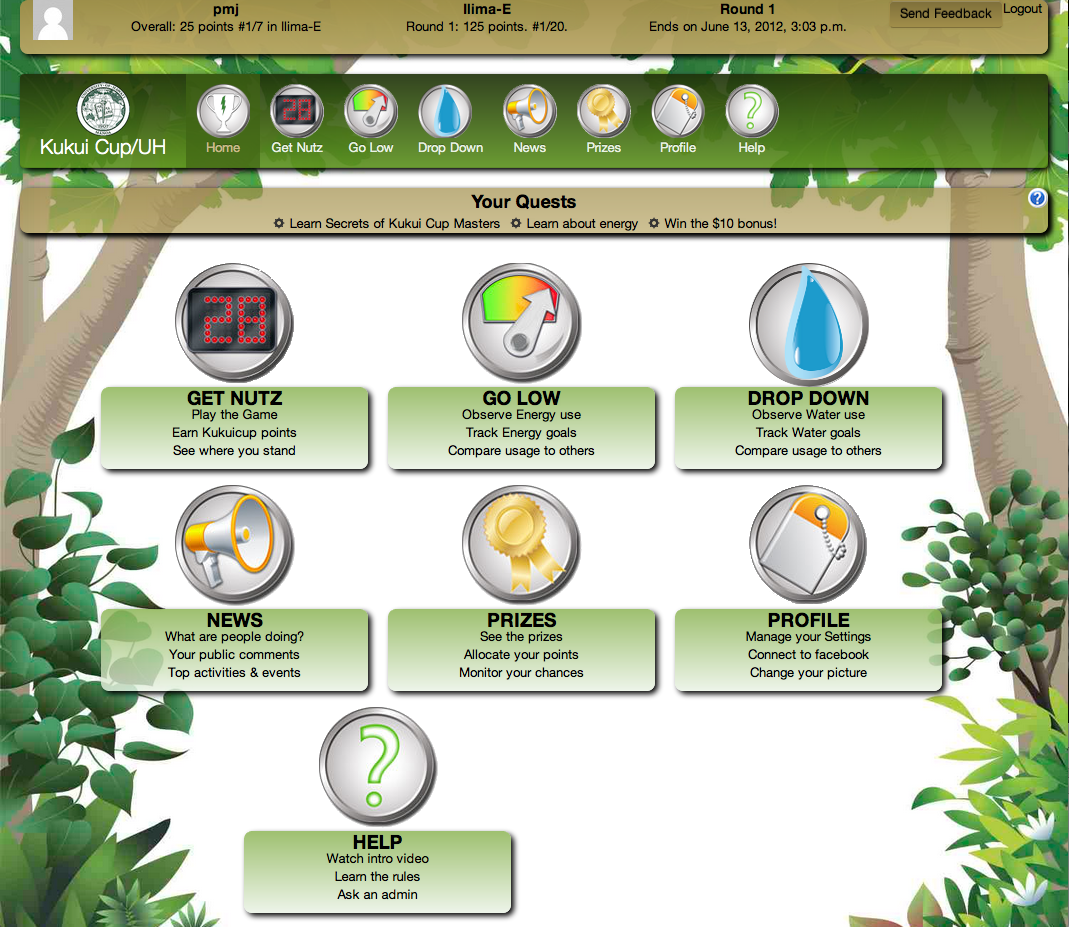
\epsfig{file=guided-tour-home, width=0.7\columnwidth}
\end{center}
\caption{Home page}
\label{fig:makahiki-home}
\end{figure}

There are three UI components in the home pages that are also appear on every page. They are:

\begin{itemize}
  \item The ``Info Bar'' is a horizontal UI component at the top of every page. It provides status information about the challenge as well as a logout link. (The player will not normally need to logout unless they are accessing the site from a public computer.)
  \item The ``Nav Bar'' is a horizontal UI component below the Info Bar, which provides icons that link to all of the top-level pages in the system. The set of pages in the system is configurable.
  \item The ``Quest Bar'' is a horizontal UI component below the Nav Bar. It provides ``Quests'' (explained in more detail below).
\end{itemize}

\clearpage

\subsubsection{Get Nutz Page}
The ``Get Nutz'' page provides the user interface to the primary sustainability education game, also known as the ``Smart Grid Game''. Players gain points by clicking on cells in the Smart Grid UI widget, which takes them to the online or real-world educational actions such as activities, commitments and events.

Figure \ref{fig:makahiki-getnutz} shows an example of the Get Nutz page (the name of this page and any other top-level page can be configured by site administrators):

\begin{figure}[!ht]
\begin{center}
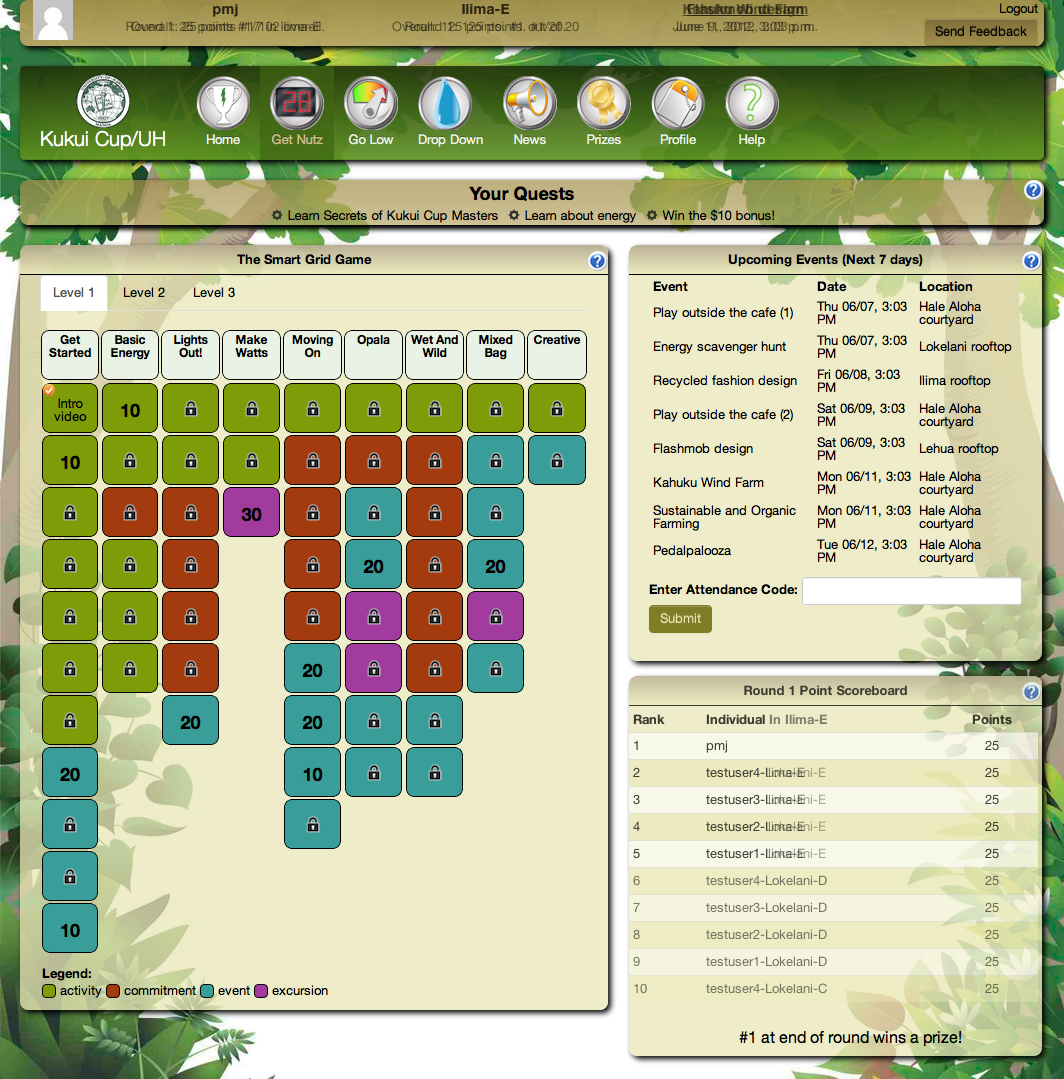
\epsfig{file=guided-tour-get-nutz, width=0.7\columnwidth}
\end{center}
\caption{Get Nutz Page}
\label{fig:makahiki-getnutz}
\end{figure}

The page also provides widgets about upcoming events and a scoreboard showing point leaders. Clicking on the link in the middle of the smart grid game takes the player to a page explaining that educational action. 

\clearpage

\subsubsection{Go Low Page}

The ``Go Low'' page provides the user interface to two ``energy'' games, as shown in Figure \ref{fig:makahiki-golow}:

\begin{figure}[!ht]
\begin{center}
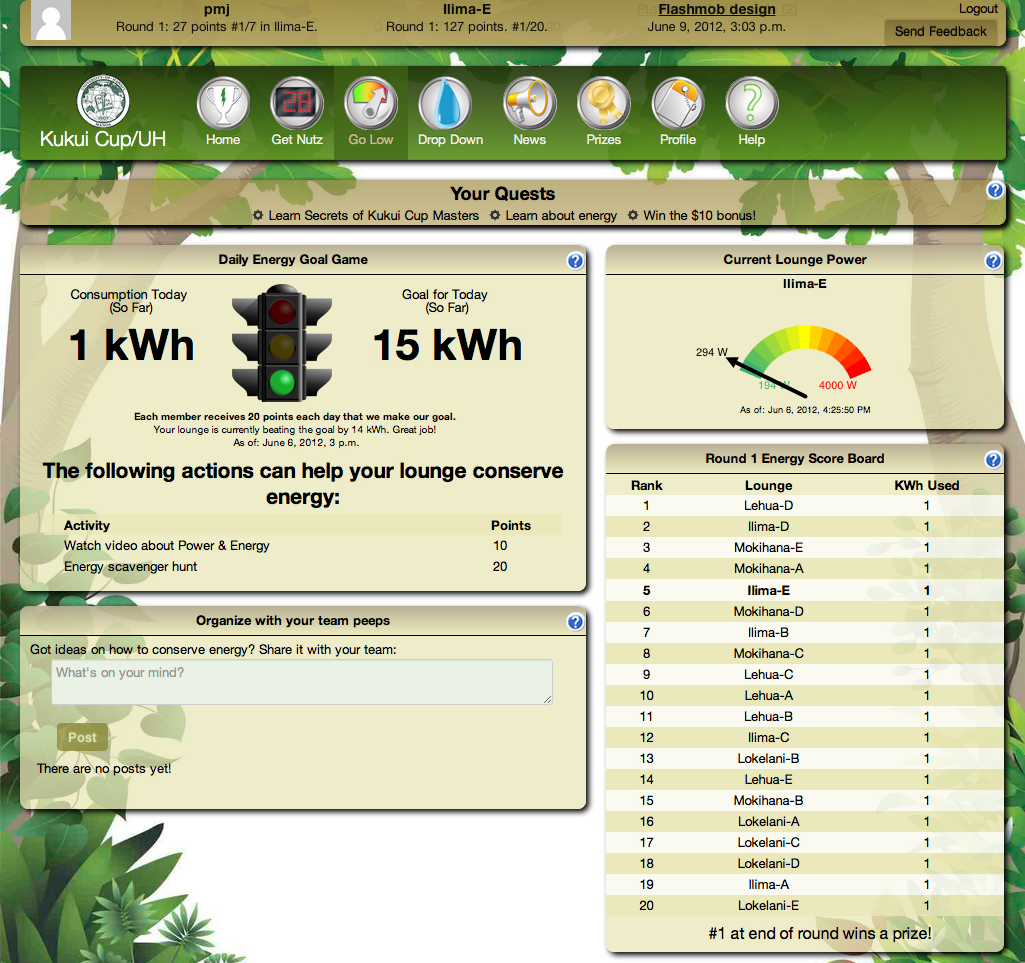
\epsfig{file=guided-tour-go-low, width=0.8\columnwidth}
\end{center}
\caption{Go Low Page}
\label{fig:makahiki-golow}
\end{figure}

On the left side, the ``Daily Energy Goal Game'' incentivizes players to reduce their energy usage by awarding them points if they can reduce their team's energy by a certain percentage below a baseline value. The stoplight visualization tells them whether or not they are currently on track to make the goal.

On the right side, the ``Current Power'' visualization helps players to see what their current power consumption is in near real-time (typically every 10-15 seconds.)

The page also enables team members to communicate via a shared chat window, and provides a scoreboard widget showing leaders in energy conservation.

\clearpage

\subsubsection{News Page}

The ``News'' page provides information about the state of the challenge and the team of which this player is a member, as shown in Figure \ref{fig:makahiki-news}:

\begin{figure}[!ht]
\begin{center}
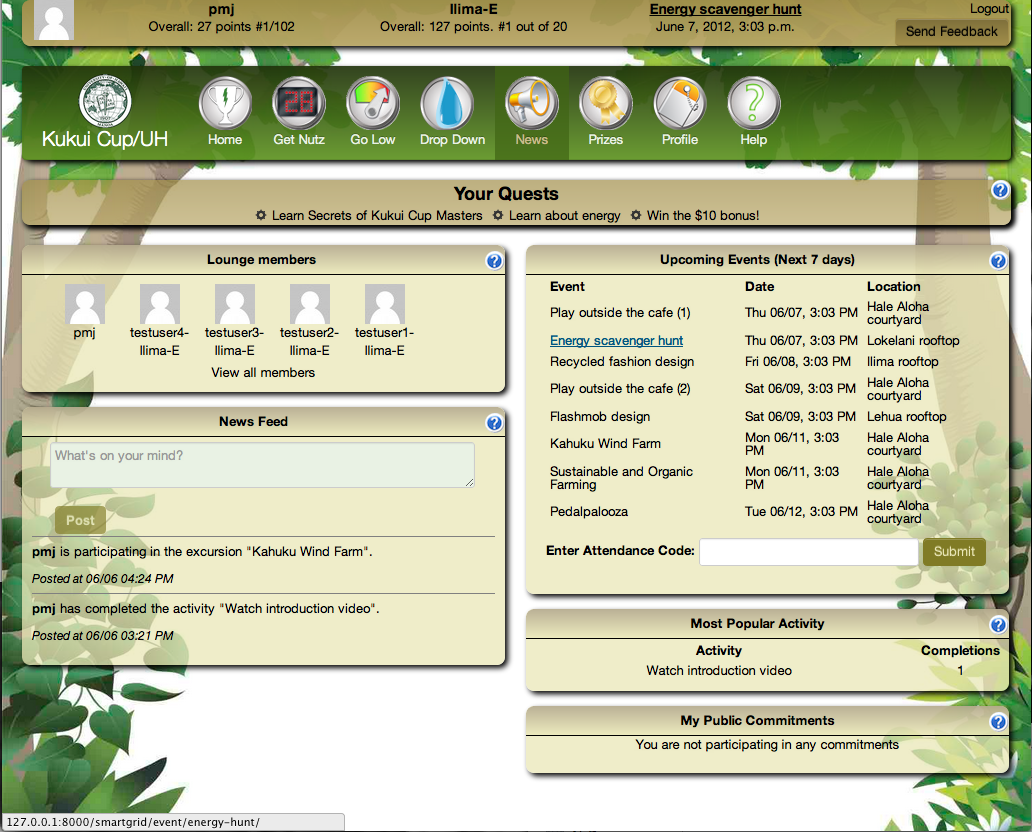
\epsfig{file=guided-tour-news, width=0.9\columnwidth}
\end{center}
\caption{News Page}
\label{fig:makahiki-news}
\end{figure}

Widgets such as ``Lounge Members'', ``Most Popular Excursion'', ``My Public Commitments'', etc. all provide a sense for the state of the competition and encourage players to participate by learning about what others members are doing.

\clearpage

\subsubsection{Prizes Page}

The ``Prizes'' page provides access to two games: the ``Top Scorer'' game and the ``Raffle'' game, as shown in Figure \ref{fig:makahiki-prizes}:

\begin{figure}[!ht]
\begin{center}
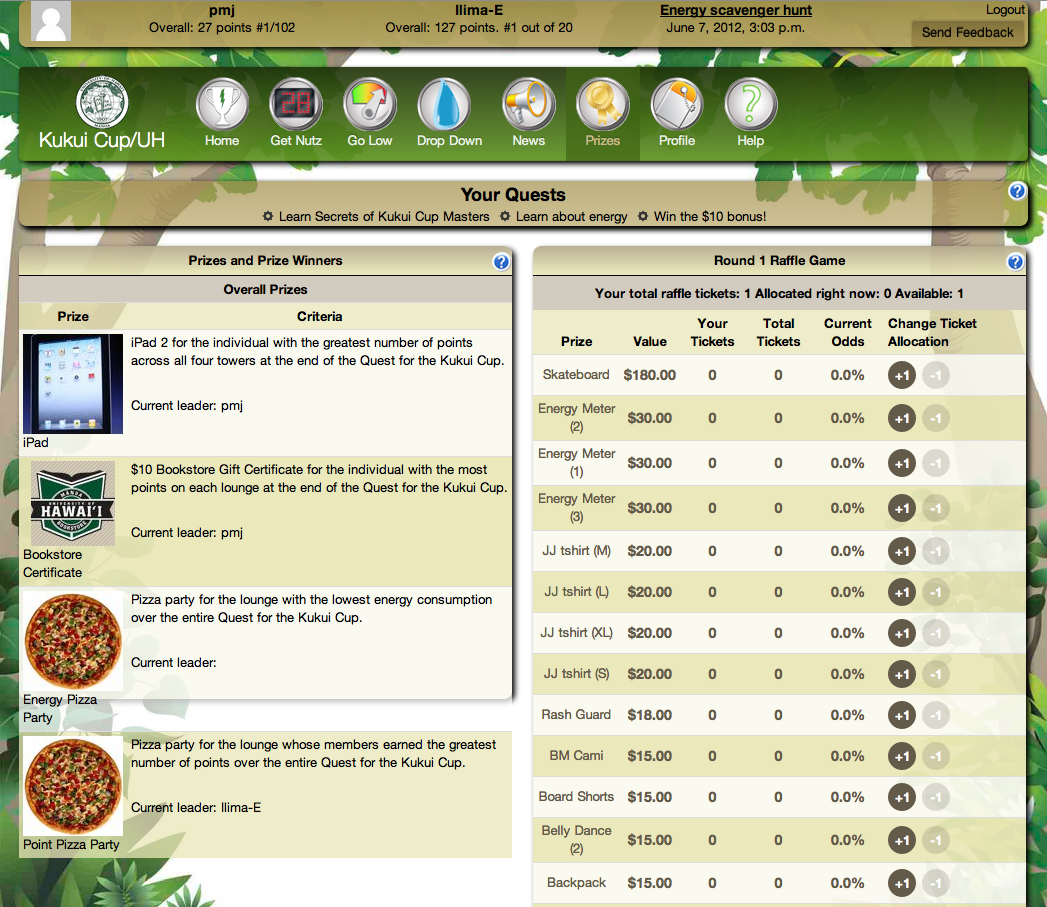
\epsfig{file=guided-tour-prizes, width=0.8\columnwidth}
\end{center}
\caption{Prizes Page}
\label{fig:makahiki-prizes}
\end{figure}

The Top Scorer game, illustrated by the widget on the left, shows the prizes that can be won by top scorers in the competition.

The Raffle Game provides an alternative route to winning. Here, players earn in-game raffle tickets based upon their point score that can be allocated to any of a collection of raffle prizes. The odds of winning are based upon the percentage of their tickets allocated to the prize, which is picked at random at the end of a round by administrators.

The Raffle Game provides an incentive for players to do activities and earn points even if they do not stand a chance of winning one of the Top Scorer prizes.

\clearpage

\subsubsection{Profile Page}

The ``Profile'' page provides access to profile information for this player, as shown in Figure \ref{fig:makahiki-profile}:

\begin{figure}[!ht]
\begin{center}
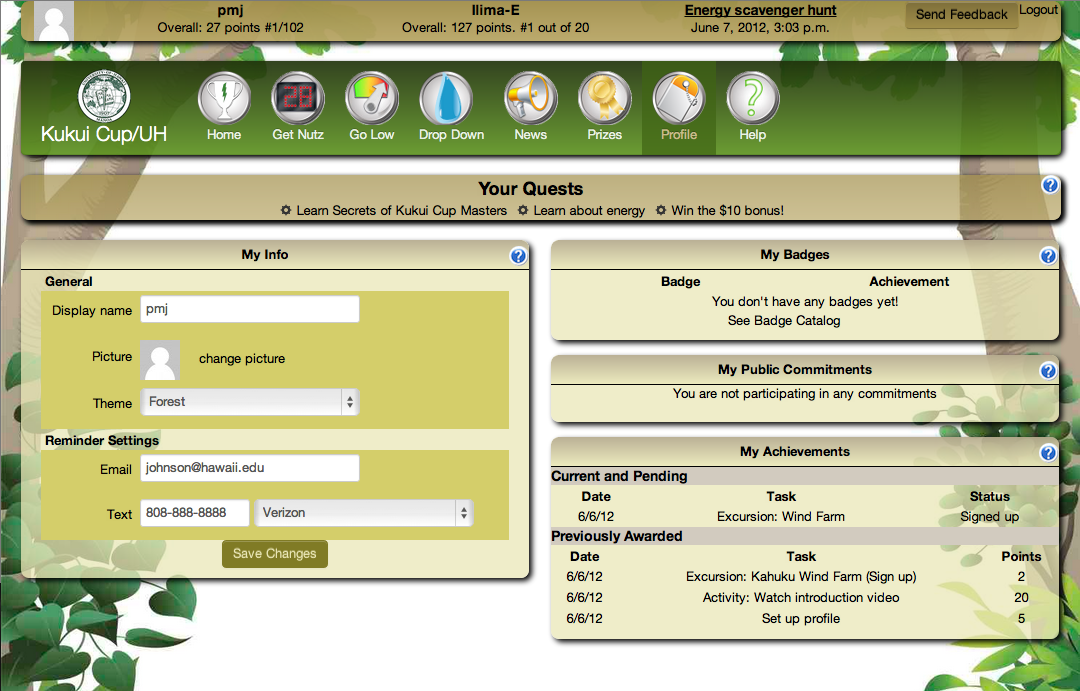
\epsfig{file=guided-tour-profile, width=0.9\columnwidth}
\end{center}
\caption{Profile Page}
\label{fig:makahiki-profile}
\end{figure}

The user can set their display name, their picture, and how they wish to be contacted for reminders. It also shows information about their badges and a complete record of how they earned all of the points in the game.

The profile page also allows them to change the theme associated with the site. A variety of themes are available. In this configuration, the default theme is ``Forest'', but the user can go to the Profile page to set a different them for their own use. 

\clearpage

\subsubsection{Help Page}

The final page available to players is the Help page, which simply provides access to explanatory material about the system, as shown in Figure \ref{fig:makahiki-help}:

\begin{figure}[!ht]
\begin{center}
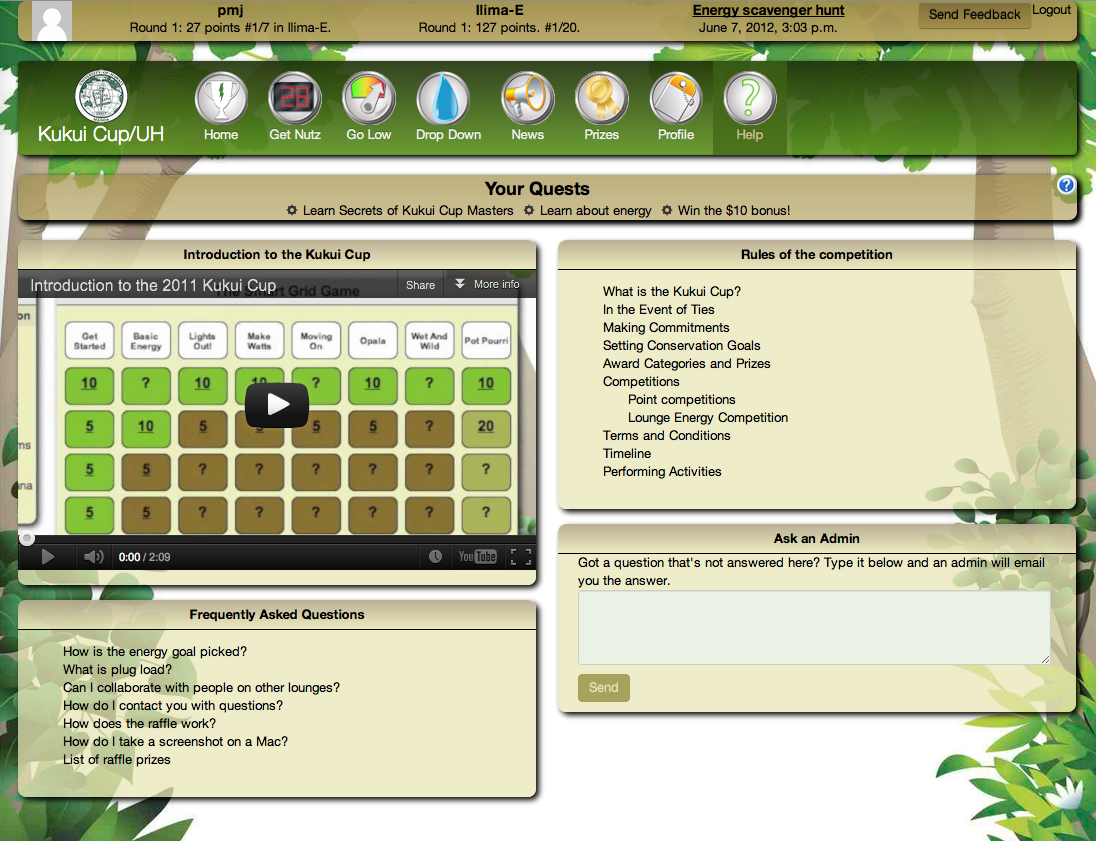
\epsfig{file=guided-tour-help, width=0.9\columnwidth}
\end{center}
\caption{Help Page}
\label{fig:makahiki-help}
\end{figure}

\clearpage

\subsection{Admin Interface}
The admin interface is used by System admin, Game designers, Game managers and Developers.

\subsubsection{Settings Page}

The settings page is restricted to administrators, as shown in Figure \ref{fig:makahiki-settings}: 

\begin{figure}[!ht]
\begin{center}

\epsfig{file=guided-tour-settings, width=0.9\columnwidth}
\end{center}
\caption{Settings Page}
\label{fig:makahiki-settings}
\end{figure}

Administrators use the Settings page to configure the site, design the challenge, manage a running challenge, generate analytics after the challenge is over, and support new development. 

\clearpage

\subsubsection{Smart Grid Game Designer Page}

The Smart Grid Game Designer page is also restricted to administrators, specifically, the game designers. It is designed to to help build the Smart Grid Game, as shown in Figure \ref{fig:makahiki-designer}:

\begin{figure}[!ht]
\begin{center}
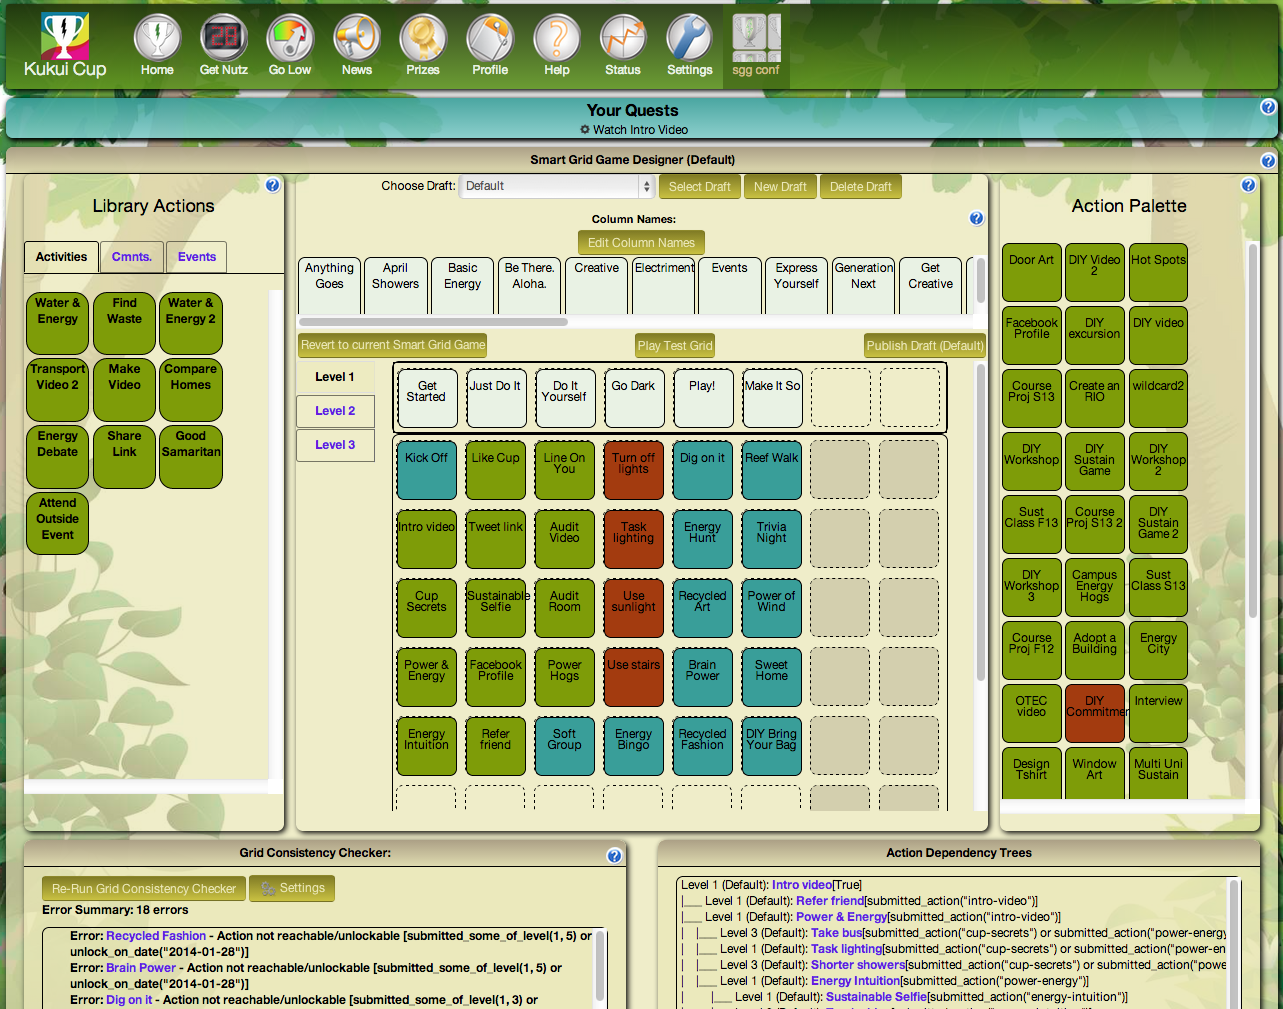
\epsfig{file=guided-tour-designer, width=0.9\columnwidth}
\end{center}
\caption{Smart Grid Game Designer Page}
\label{fig:makahiki-designer}
\end{figure}

Game designers use this page to construct the Smart Grid Game, by dragging and dropping the squares (game actions) into the grid with the intended layout.

\clearpage

\subsubsection{Status Page}

The ``Status'' page, also restricted to administrators, displays a large number of different widgets with various kinds of information about the state of an ongoing challenge. Figure \ref{fig:makahiki-status} shows a screenshot of part of the Status page:

\begin{figure}[!ht]
\begin{center}
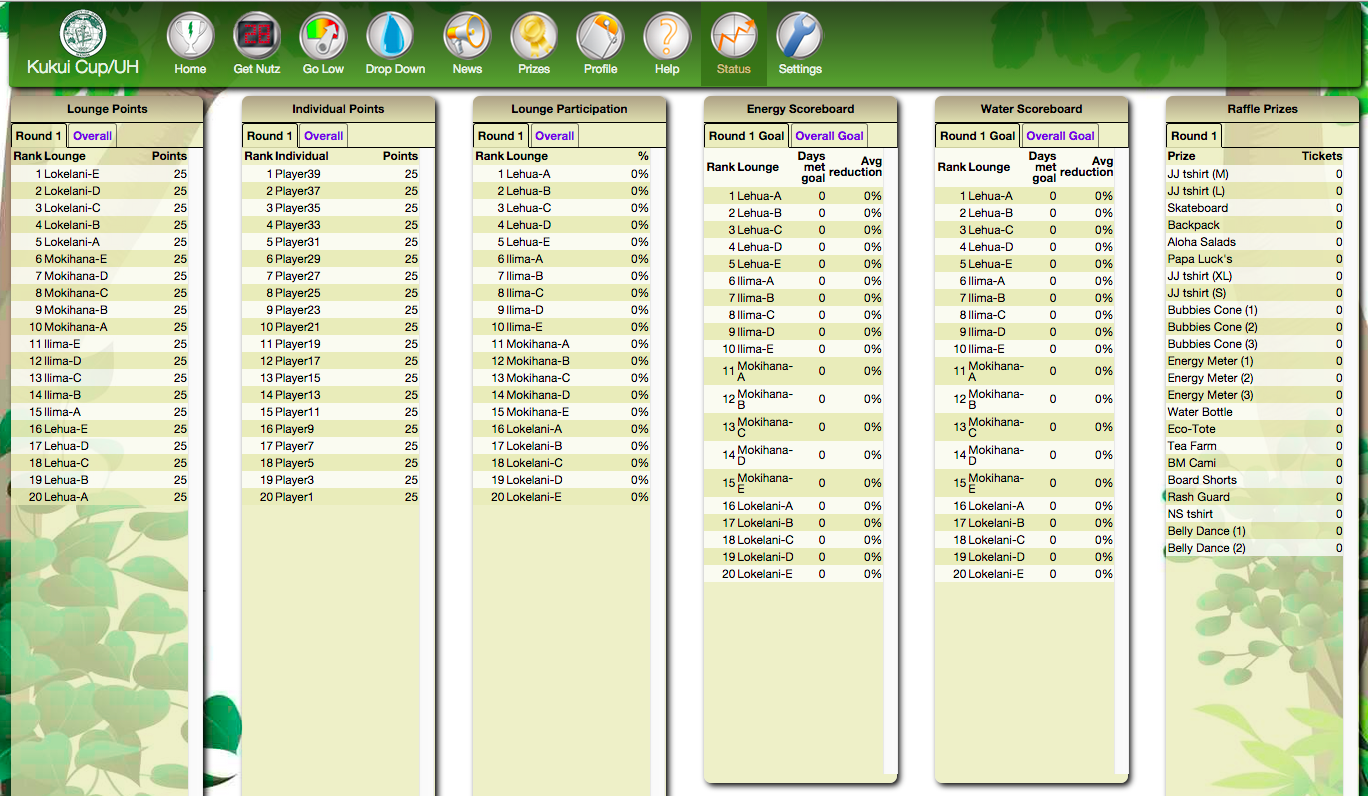
\epsfig{file=guided-tour-status, width=0.9\columnwidth}
\end{center}
\caption{Status Page}
\label{fig:makahiki-status}
\end{figure}

The Status page is designed to help administrators to monitor the progress of their challenge, detect problems with the system and/or state of play, and intercede to correct them in a timely manner.

\clearpage

\section{System Design}

\subsection{Architecture}

Figure \ref{fig:makahiki-architecture} illustrates the overall architecture of Makahiki.

\begin{figure}[!ht]
\begin{center}
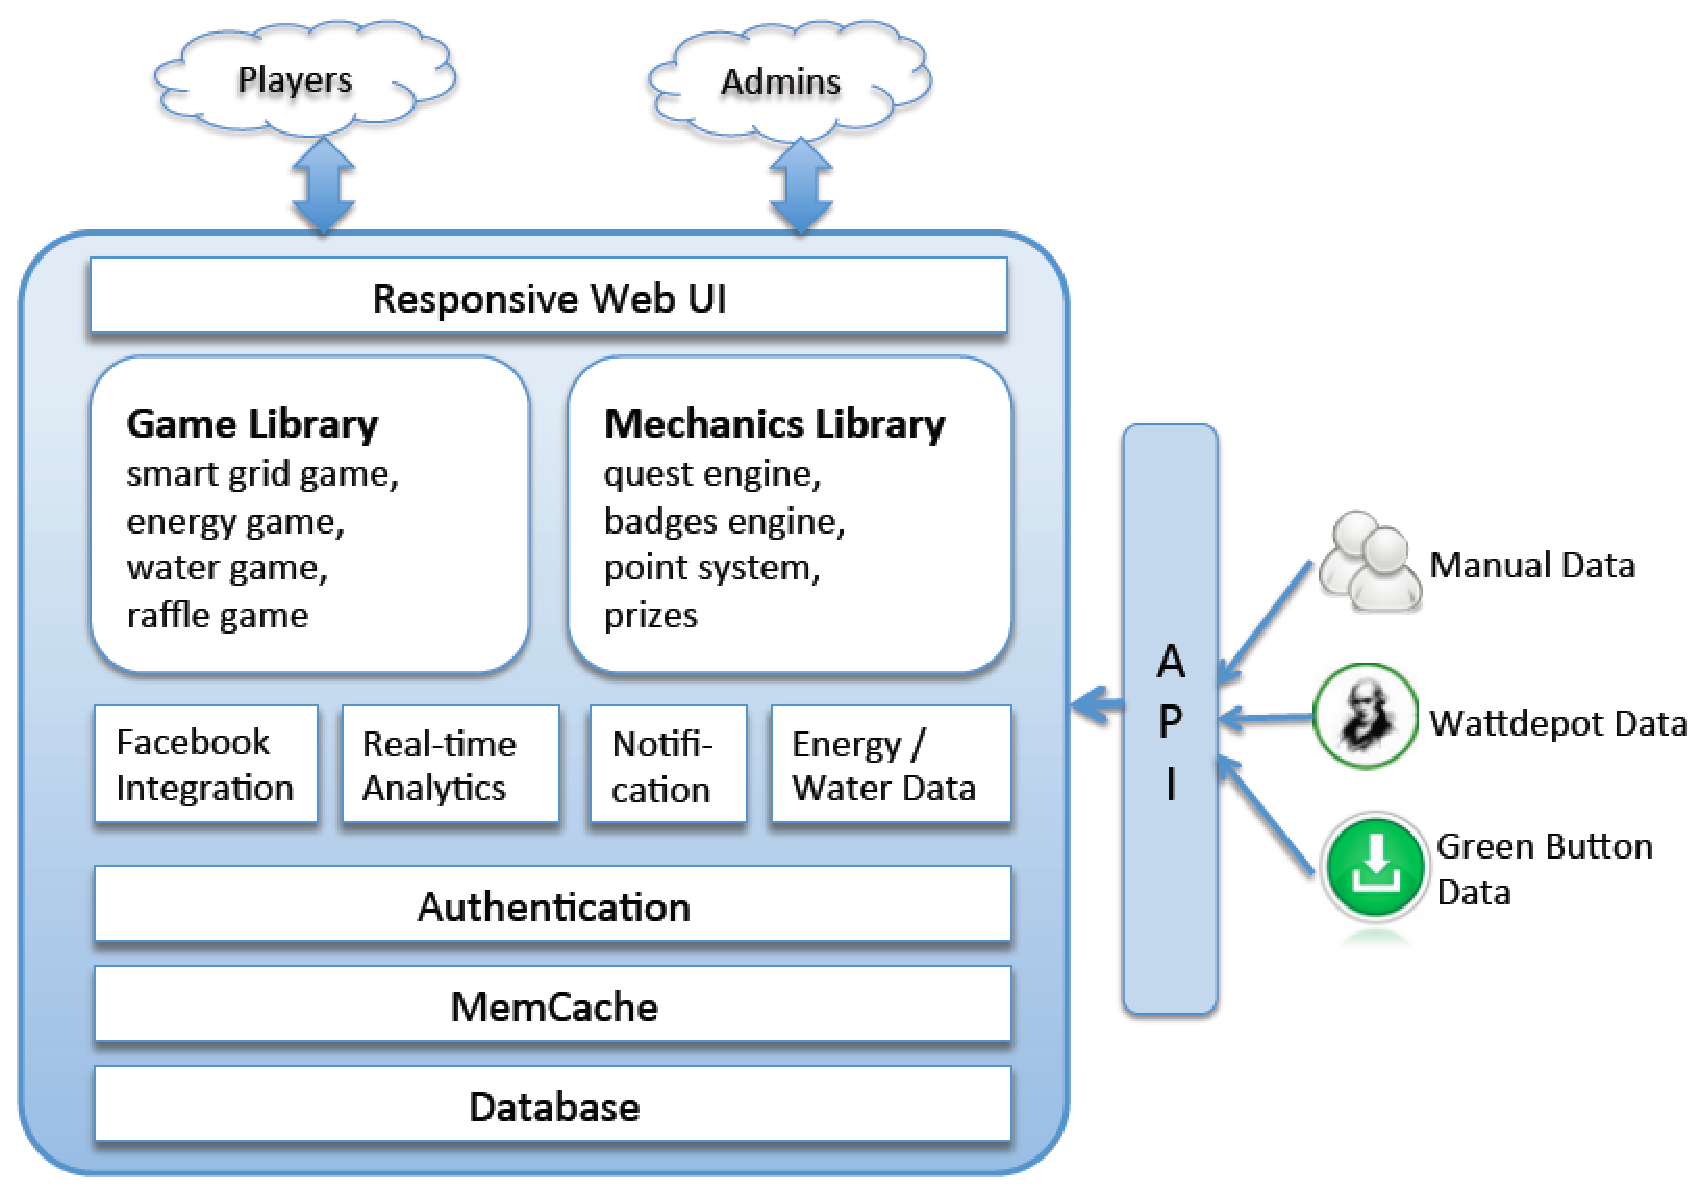
\epsfig{file=makahiki-system-architecture, width=0.8\columnwidth}
\end{center}
\caption{Architecture of Makahiki}
\label{fig:makahiki-architecture}
\end{figure}

The core component of Makahiki is a configurable game engine that can be customized to the needs of different organizations.  It includes two libraries of games and game mechanics. These libraries consists of a set of pre-built ``widgets''. By selecting and configuring these game and game mechanics widgets, an organization can create a customized energy and water challenge (or serious game) in which players compete both individually and in teams, earn points by reducing their energy consumption as well as by learning about energy concepts in general, with the incentives such as top score prizes and raffle prizes.  

Makahiki interfaces with the outside environment in third different ways.

First, the top side of the architecture diagram shows that Makahiki has two primary user interfaces: one for the players of the serious game, who directly interact with the game and game mechanics widgets; the other for the administrators of the system, who configure the system and monitor the real-time game analytics.

Second, the right side of the diagram illustrates that Makahiki must obtain real-world environmental data as the challenge progresses in order to provide feedback to users about the impact of their actions. In some cases, environmental data can be input automatically into the system through a combination of ``smart'' meters and additional services (such as the WattDepot system for energy data collection, storage, and analysis). If that is not possible, then manual meters can be read by administrators on a regular (typically daily) basis and input into Makahiki using and administrator interface.

Third, the bottom side illustrates that Makahiki stores its data in a database repository (currently PostgreSQL). To reduce database access and improve performance, Makahiki provides support for caching (currently memcached).

Figure \ref{fig:makahiki-internal-architecture} illustrates the internal architecture of Makahiki. It provides a perspective on Makahiki's internal architecture in terms of three kinds of ``components'': Django-related infrastructure, Widgets, and Managers.

\begin{figure}[!ht]
\begin{center}
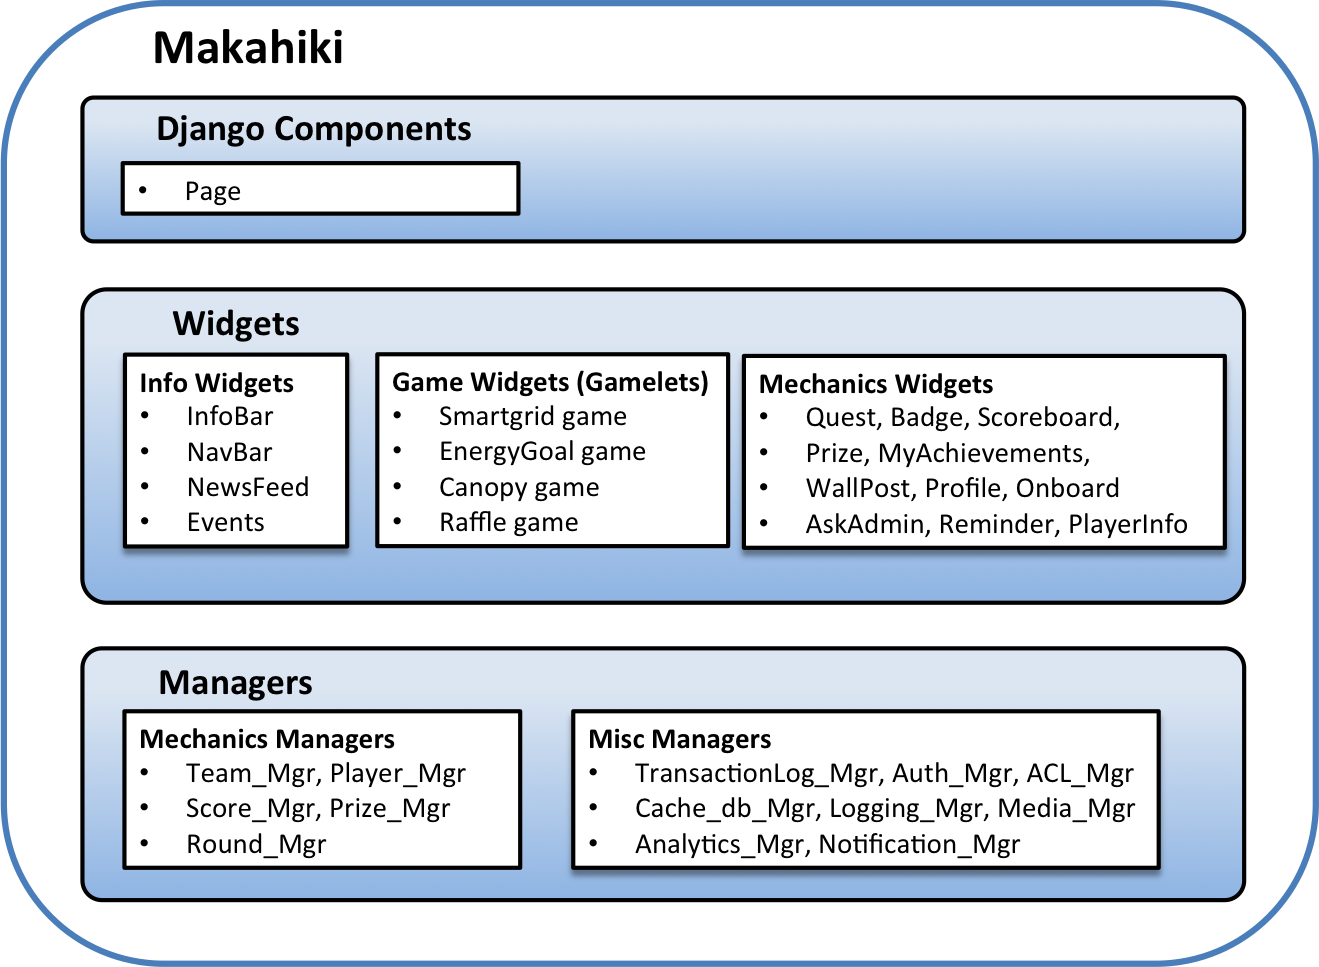
\epsfig{file=makahiki-internal-architecture, width=0.7\columnwidth}
\end{center}
\caption{Internal Architecture of Makahiki}
\label{fig:makahiki-internal-architecture}
\end{figure}

Managers are modules that provide Makahiki capabilities that do not involve a (player) user interface. They might provide interaction with administrators via the Django admin interface. Managers can implement game mechanic data structures (such as scores, players, and teams) or more generic web service functions (transactions, authorization, etc.)

\begin{table}[ht!]
  \centering
  \begin{tabular}{|c|c|c|}
    \hline
    \multicolumn{1}{|p{0.2\columnwidth}|}{\centering\tabhead{Manager}} &
    \multicolumn{1}{|p{0.2\columnwidth}|}{\centering\tabhead{Module Name}} &
    \multicolumn{1}{|p{0.5\columnwidth}|}{\centering\tabhead{Functionality}} \\
    \hline
    \multicolumn{1}{|p{0.2\columnwidth}|}{Authentication Manager} &
    \multicolumn{1}{|p{0.2\columnwidth}|}{auth\_mgr} &
    \multicolumn{1}{|p{0.5\columnwidth}|}{Provides authentication services for Makahiki including administrative logins and CAS authentication} \\
    \hline
    \multicolumn{1}{|p{0.2\columnwidth}|}{Cache Manager} & 
    \multicolumn{1}{|p{0.2\columnwidth}|}{cache\_mgr} &
    \multicolumn{1}{|p{0.5\columnwidth}|}{Manages caching data structures} \\
    \hline
    \multicolumn{1}{|p{0.2\columnwidth}|}{Challenge Manager} &
    \multicolumn{1}{|p{0.2\columnwidth}|}{challenge\_mgr} &
    \multicolumn{1}{|p{0.5\columnwidth}|}{Maintains state information about an entire Challenge, including what widgets are enabled, the round information} \\
    \hline
    \multicolumn{1}{|p{0.2\columnwidth}|}{Log Manager} &
    \multicolumn{1}{|p{0.2\columnwidth}|}{log\_mgr} &
    \multicolumn{1}{|p{0.5\columnwidth}|}{Provides logging services to track the actions of logged in users} \\
    \hline
    \multicolumn{1}{|p{0.2\columnwidth}|}{Player Manager} &
    \multicolumn{1}{|p{0.2\columnwidth}|}{player\_mgr} &
    \multicolumn{1}{|p{0.5\columnwidth}|}{Supports definition and processing of players} \\
    \hline
    \multicolumn{1}{|p{0.2\columnwidth}|}{Resource Manager} &
    \multicolumn{1}{|p{0.2\columnwidth}|}{resource\_mgr} &
    \multicolumn{1}{|p{0.5\columnwidth}|}{Provides supports for resource management, such as updating energy or water data, checking daily goals} \\
    \hline
    \multicolumn{1}{|p{0.2\columnwidth}|}{Score Manager} &
    \multicolumn{1}{|p{0.2\columnwidth}|}{score\_mgr} &
    \multicolumn{1}{|p{0.5\columnwidth}|}{Manages score keeping, scoreboard calculation} \\
    \hline
    \multicolumn{1}{|p{0.2\columnwidth}|}{Team Manager} &
    \multicolumn{1}{|p{0.2\columnwidth}|}{team\_mgr} &
    \multicolumn{1}{|p{0.5\columnwidth}|}{Support definition and management of teams} \\
    \hline
  \end{tabular}
  \caption{Makahiki Internal Manager Modules}
  \label{table:managers}
\end{table}

Widgets are modules that provide Makahiki capabilities that do include a player user interface. Widgets can be roughly characterized in three ways. ``Info widgets'' provide state information about the challenge to players but little in the way of interaction. ``Mechanics widgets'' provide game elements such as Quests and Badges. The third category, ``game widgets'', refer to full-fledged interactive games.

\subsection{A Library of Configurable Games and Mechanics}

Makahiki builds in a set of configurable games and mechanics that can be turned on or off, or customized by the game designers to the needs of different organizations. The rest of this section describes these games and game mechanics and how to configure them.

\subsubsection{Selecting a Game or Game Mechanics from the Library}
A challenge designer can decide which of the built-in game and mechanics will appear in a sustainability challenge for his organization. The challenge design setting page includes a widget called ``Game Settings'', which lists the set of games available and whether or not they are currently enabled, as is shown in Figure \ref{fig:game-display-widget}.

\begin{figure}[!ht]
  \center
  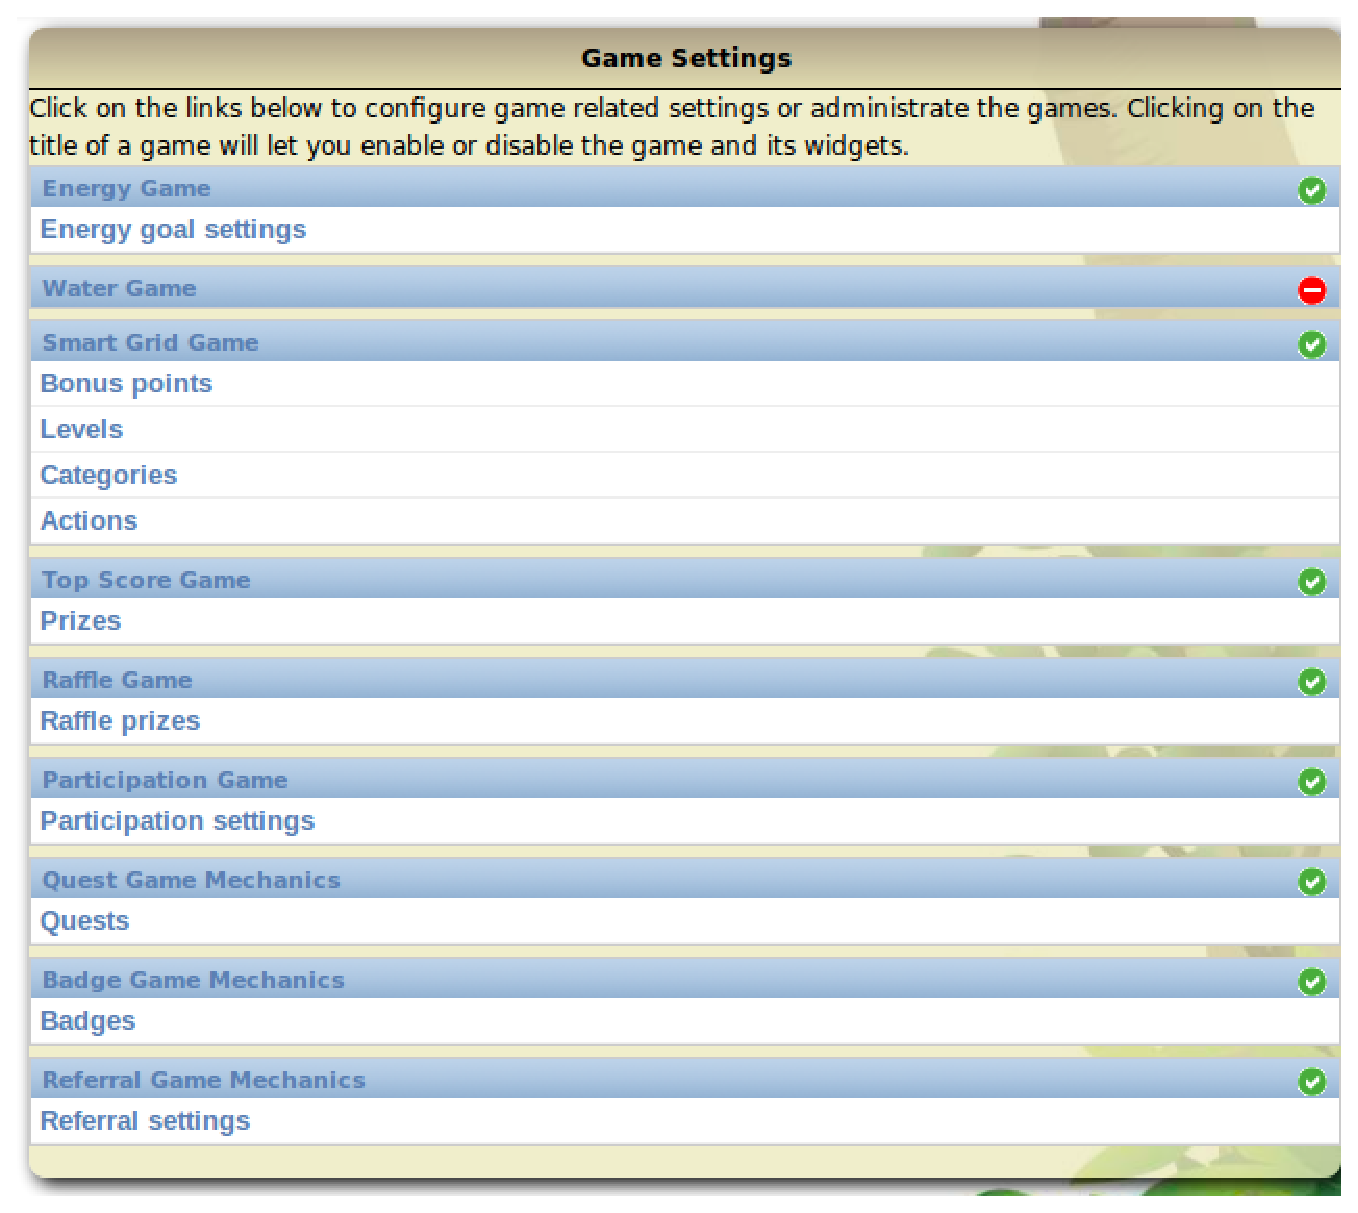
\includegraphics[width=0.7\columnwidth]{game-display-widget.eps}
  \caption{\em Selecting a Game from Game Settings}
  \label{fig:game-display-widget}
\end{figure}

The small green and red icons on the right side indicate whether a game is currently enabled for the challenge. In this case, all of the games but one (Water Game) are enabled. Clicking on the title of a game will let you enable or disable the game and its widgets. After clicking on the title link in the Game Admin widget, a page similar to the Figure \ref{fig:game-settings} will appear:

\begin{figure}[!ht]
  \center
  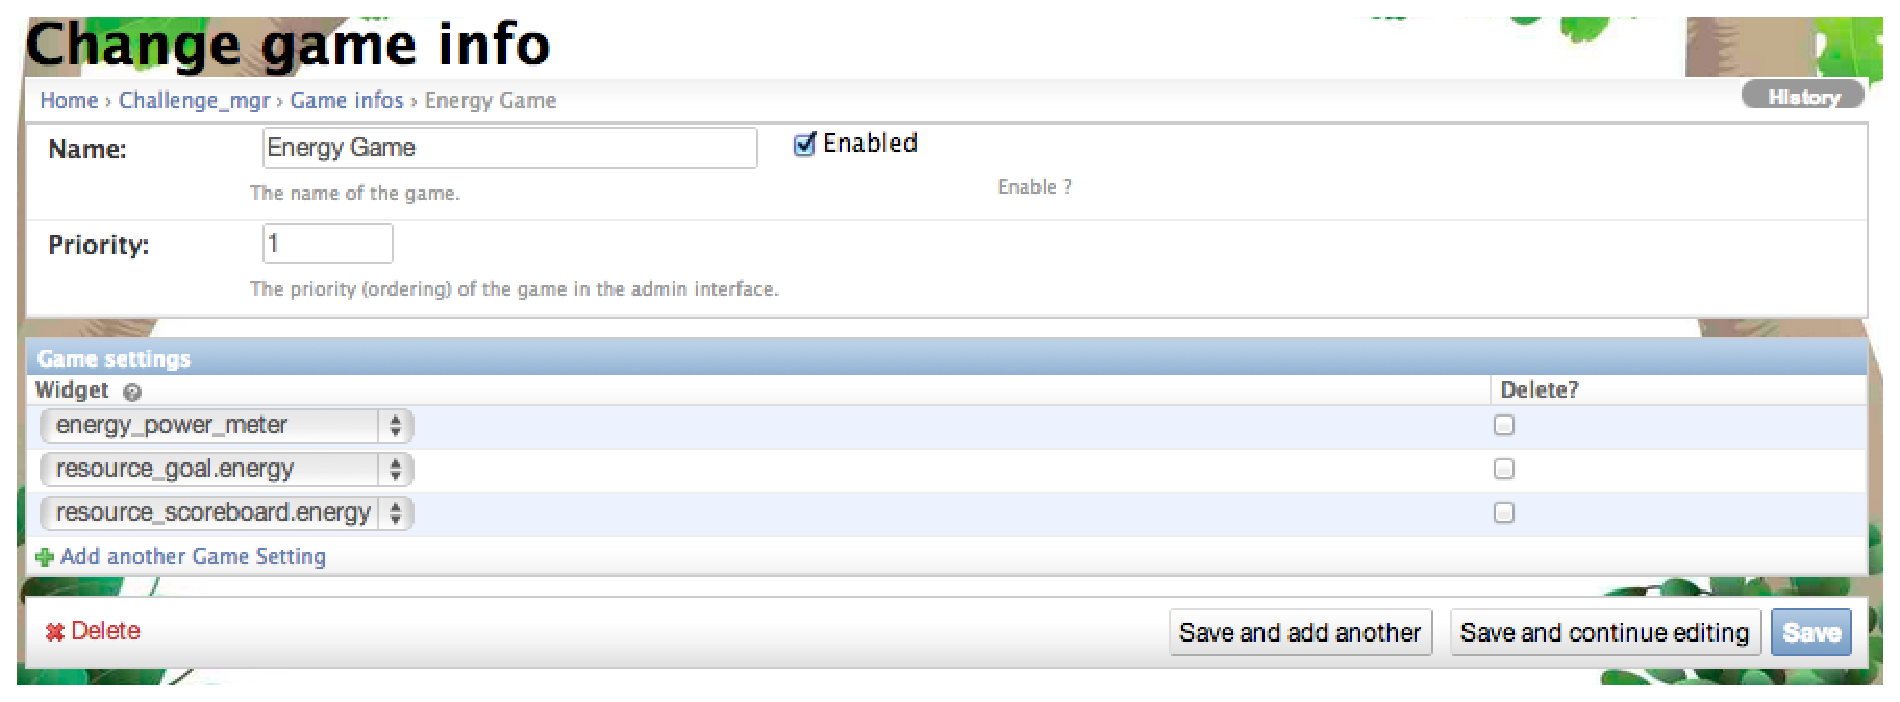
\includegraphics[width=0.8\columnwidth]{game-settings.eps}
  \caption{\em Change a Game's Setting}
  \label{fig:game-settings}
\end{figure}

You can check or uncheck the ``enabled'' checkbox to enable or disable the game.

A game's UI is represented by a set of widgets which is visible in the game website. The widgets belong to a game is listed under the “Game Settings” section, as shown from the above screen shot. If you disable the game, all the widgets belong to this game will not be shown in the web page.

Makahiki currently allows you to create a challenge out of the following games and game mechanics:

\begin{itemize}

\item {\em Energy Game}. This game awards points to players depending upon their ability to lower their energy consumption.

\item {\em Water Game}. This game awards points to players depending upon their ability to lower their water consumption.

\item {\em Smart Grid Game}. This game is the principle interface to the educational component of Makahiki. The SGG awards points to players for successfully completing activities, commitments, excursions, and events.

\item {\em Top Score Game}. This game awards prizes to players and teams for earning the highest number of points during a round.

\item {\em Raffle Game}. This game awards prizes to players if they have allocated their raffle tickets to a particular raffle prize, and that raffle ticket was randomly selected by the system at the end of a round.

\item {\em Participation Game}. This game awards points to players if they can successfully get a certain percentage of their team members to participate in the challenge.

\item {\em Quest Game Mechanics}. This game mechanic provides a way for players to learn about features of the challenge by guiding them through Quests.

\item {\em Badge Game Mechanics}. This game mechanic provides a way for players to earn badges for playing the game in a variety of ways.

\item {\em Referral Game Mechanics}. This game mechanic provides a way for players to earn points by getting other people to participate in the challenge.

\end{itemize}

The following sections explain the design and configuration of each game and game mechanics.

\subsubsection{Energy and Water Game}

A fundamental requirement for enabling more active participation in sustainability behavior is feedback regarding their resource such as energy and water usage. The Energy and Water game in Makahiki are implemented as the Daily Resource Goal Game, which includes Daily Energy Goal Game and Daily Water Goal Game.

The Daily Energy Goal Game widget provides a way for players to see the outcome of the energy reduction behavior, and to make it a game by earning points from their behavior. By reducing their teams' daily energy consumption from a baseline by a set percentage, the players in the team will all earn the configured amount of points. This baseline is calculated using historical data and dynamically throughout the competition. Both the baseline data and the current consumption is typically provided by API calls from Makahiki to an underlying WattDepot server.
Figure \ref{fig:DailyEnergyGoal} illustrates this widget.

\begin{figure}[!ht]
  \center
  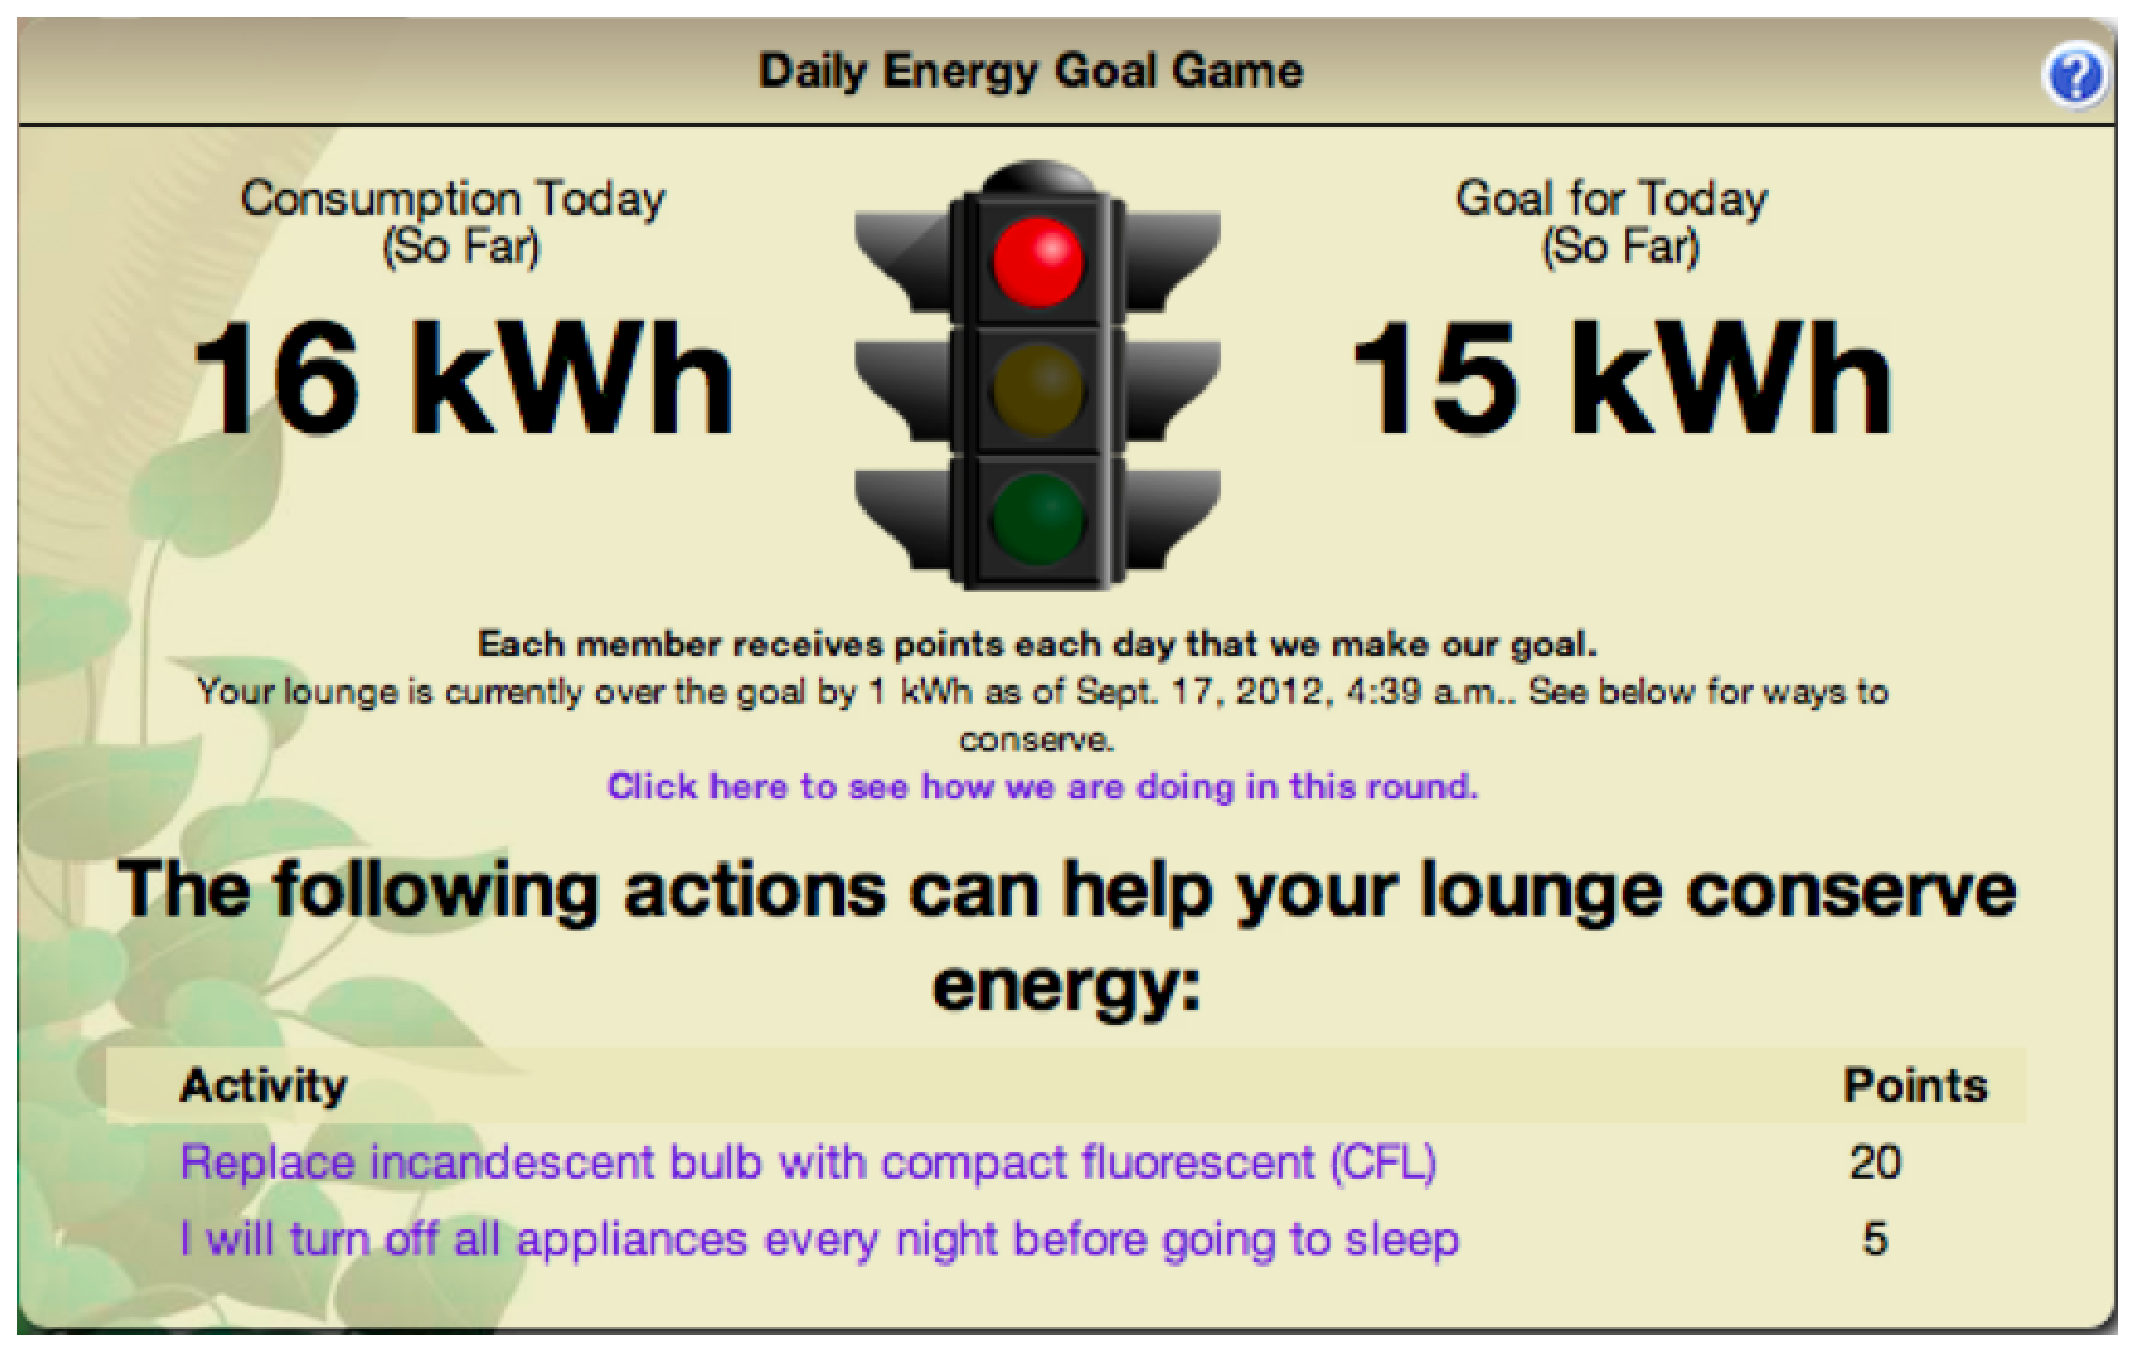
\includegraphics[width=0.6\columnwidth]{daily-energy-goal-game.eps}
  \caption{\em Daily Energy Goal Game widget}
  \label{fig:DailyEnergyGoal}
\end{figure}

As you can see, this interface uses a stoplight metaphor to show at a glance whether or not the team is making the goal. In this case, the stoplight is green, indicating they are currently below the goal.

The goal for each team is typically a percent reduction from their baseline usage. When a player goes to the ``Go Low'' page of Makahiki, they can view their team's current progress toward their daily energy goal. Near the end of the day, Makahiki checks the energy data from Wattdepot to see if a floor reached their goal. If the floor did reach their goal, each member of the floor that is participating in the game receives points. The energy goal game provides a link between the energy conservation competition and the point competition.

While the stoplight visualization provides good feedback to a team regarding their current progress toward making the current day's goal, we have found additional perspectives to also be useful.

One useful perspective to a team is a realtime power meter visualization that shows the current power usage of a team, as shown in Figure\ref{fig:PowerMeter}.

\begin{figure}[!ht]
  \center
  
\includegraphics[width=0.45\columnwidth]{power-meter.eps}
  \caption{\em Power Meter widget}
  \label{fig:PowerMeter}
\end{figure}

This visualization displays the realtime power consumption which updates in a specified interval. This give players the sense of energy consumption at the moment. For example, someone turns on a high power microwave, they might see a spike in the realtime power meter reflecting the power usage at that moment.

Another useful perspective to a team is a historical, calendar-based visualization that shows the results of the energy goal game for each day of the current round, as shown in Figure\ref{fig:degg-calendar}.

\begin{figure}[!ht]
  \center
  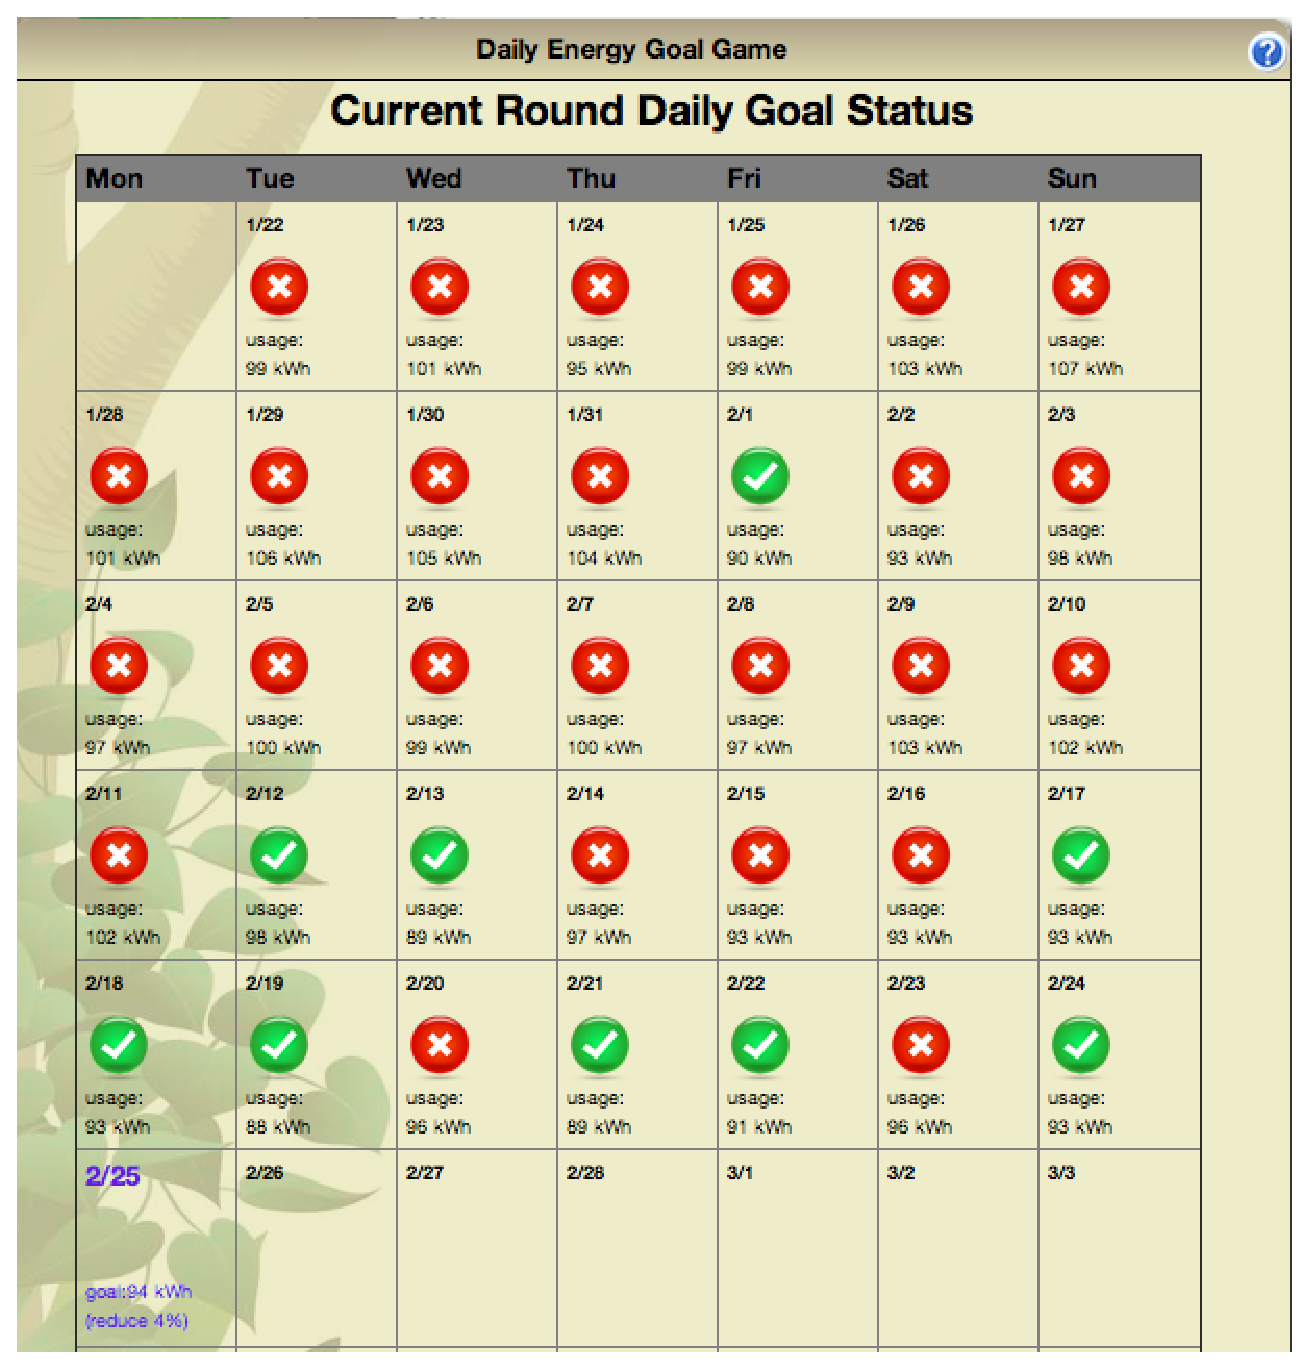
\includegraphics[width=0.6\columnwidth]{degg-calendar.eps}
  \caption{\em Daily Energy Goal Game Calendar widget}
  \label{fig:degg-calendar}
\end{figure}

This visualization is useful for helping teams to see if there are patterns to their ability to make their goal. The above display shows that they have been making their goal more regularly in the recent past, indicating perhaps that they have identified a useful strategy for conservation.

Yet another perspective of the energy consumption is illustrated in Figure \ref{fig:degg-scoreboard}. It is the Daily Energy Goal Game Scoreboard, which shows how teams are faring relative to each other. It can incentivize teams to conserve not only to earn points, but also to do better than other teams as respective energy consumption. The scoreboard shows that the number of times that a team makes their daily energy goal and the average reduction percentage.

\begin{figure}[!ht]
  \center
  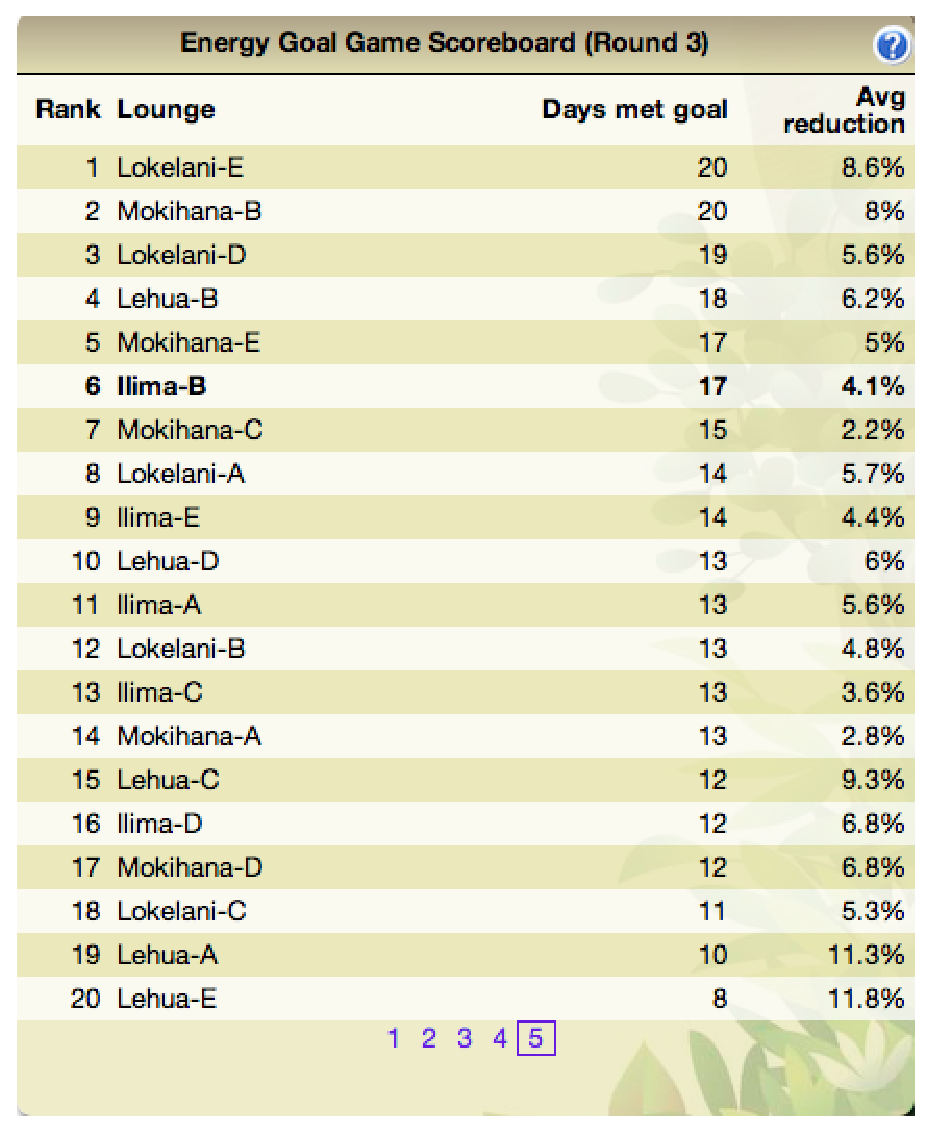
\includegraphics[width=0.5\columnwidth]{degg-scoreboard.eps}
  \caption{\em Daily Energy Goal Game Scoreboard}
  \label{fig:degg-scoreboard}
\end{figure}

The Daily Water Goal Game is similar to the Energy Goal game, with the only difference is the data, and whether the data is automatically or manually collected. With the installation of smart water meter and the availability of automatic data collection system, all the visualization discussed above will be available to the Water game. Otherwise, the water consumption data have to be manually input daily. In this case, the hourly Water Goal Game widget and the near realtime Power Meter widget will not be available to the players, while the daily water scoreboard widget and calendar view widget will be available.

\clearpage

\subsubsection{Smart Grid Game}

Smart Grid Game (SGG) is Makahiki's approach to support ``gamified'' delivery of educational experiences. It is the primary place players go to learn about sustainability issues and earn points. Educational actions are organized into a grid of squares (hence the name ``Smart Grid'') and organized by category columns and levels. Players use its grid interface to discover ``actions'' they can perform. Successful completion of an action earns the player a variable number of points depending upon the difficulty of the action, and can potentially ``unlock'' additional actions and higher levels in the SGG. Figure \ref{fig:SmartGrid} shows a typical Smart Grid Game interface for players:

\begin{figure}[!ht]
  \center
  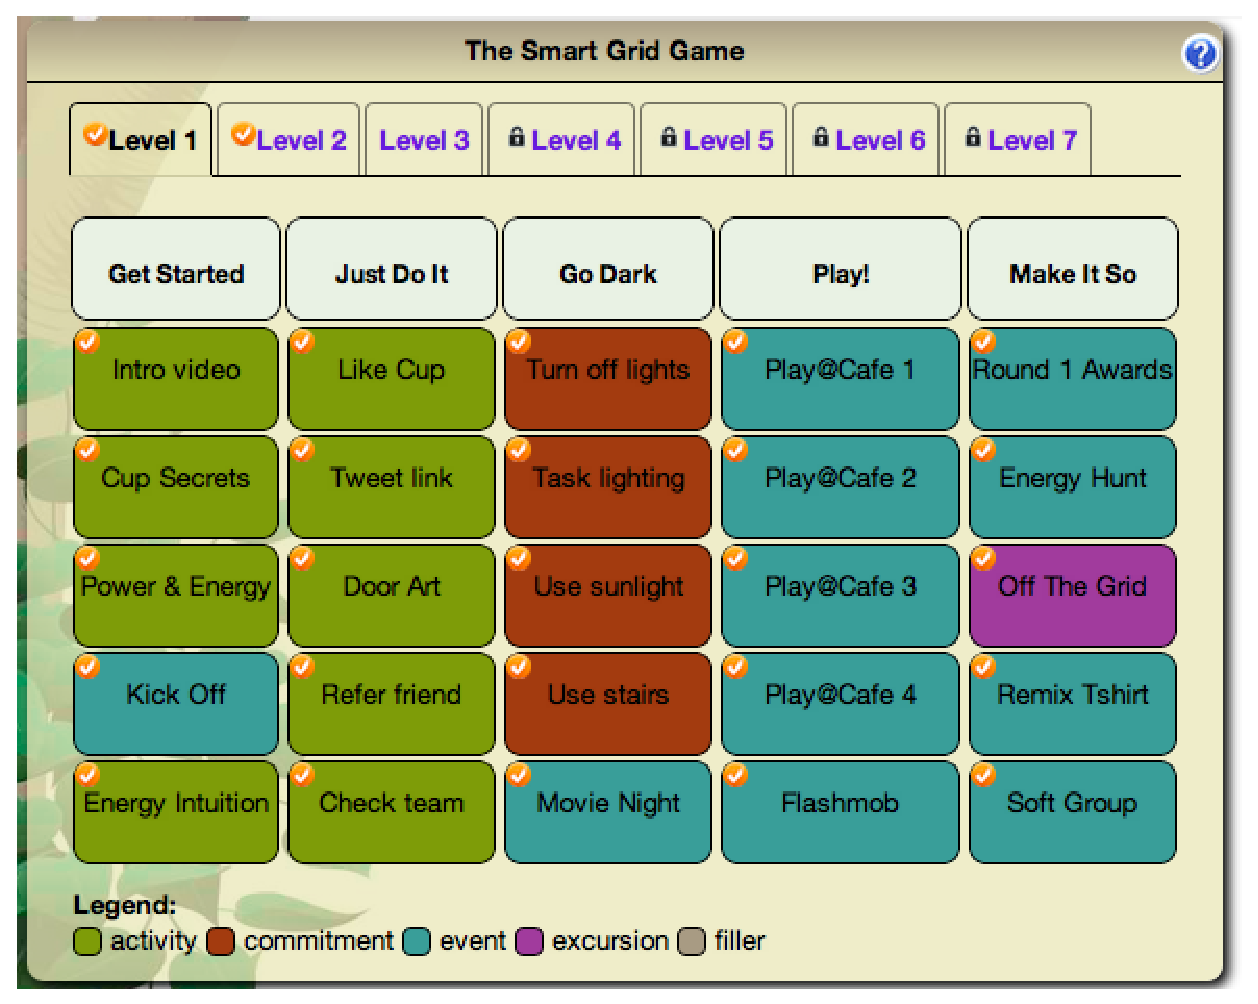
\includegraphics[width=0.6\columnwidth]{smart-grid.eps}
  \caption{\em Smart Grid Game widget}
  \label{fig:SmartGrid}
\end{figure}

There are three types of actions in the grid:

{\em Activities} are the most basic action available in the Smart Grid. In order to get points for an activity, a player must input a response to the system, which is reviewed and approved or disapproved by administrators. These responses can be a short textual answer or an uploaded picture. If a submission is approved, the player receives the points for their submission. Otherwise, the system notifies the player that their submission was not approved, along with a comment (written by an administrator) explaining why it was rejected. The player can change and resubmit their response and still earn the full point value for that task. 

Most activities have fixed rewarding points if completed. Creative activities are special kind of activities that worth a variable number of points, which depends on the effort made by the player and the quality of the outcome submitted. It is judged by the administrators. These activities enable players to exercise their artistic talents. 

{\em Commitments} are pledges that the player will carry out a specific action for a specific amount of time (typically 5 days). Examples include: reducing shower time, taking the stairs, and turning off the lights when leaving a room. Unlike activities, commitments are not easily verifiable, and so they are usually designed with fewer points than activities. Furthermore, a player can only enter into five commitments at any given time. After the commitment period is up, the player can declare that they completed the commitment and immediately earn the associated points. They can then enter into another commitment, including the one they just completed. 

{\em Events} are actions tied to real world meetings. To help organizers gauge interest in events, players can earn points by signing up in advance. Players that do this (and then actually attend the event) earn a signup bonus (typically 2 points). Players can also set up a reminder that is sent to their email and/or their mobile phone before the meeting takes place. At the event, a challenge administrator provides players with ``attendance codes'' printed on slips of paper that can be later entered in the system by the player to get their points. (The paper slips provide a form of verification that the player physically attended the event.) Attendance codes are generated by Makahiki and can only be used once. To discourage players from signing up and not attending, a penalty (typically 2 points) is assessed to players who do not submit an attendance code. If the player submits an attendance code for the event after receiving this penalty, the penalty is reversed. 

To make your SGG more interesting to players, and more pedagogically sophisticated, Makahiki supports the definition of ``{\em Path}'' through the educational content or actions. In most cases, when a new player sees the SGG for the first time, there should only be a few actions available to them� possibly only one. All of the rest should be locked. Makahiki provide a set of predicates that can be used to define the ``path''. The predicates  determines if an action or level is locked or unlocked for a player, which in term depends on the outcome of another action or multiple other actions. Predicates include: completed a certain number of actions within a category, completed all actions within a category, completed  a certain action, and unlocking of an action or level after a certain date.

To incentivize players to work together during a challenge, Makahiki also supports ``{\em Social Bonus}''. The social bonus is an optional attribute of any Smart Grid Game action which awards extra points if the player has done the action with someone else. Examples of actions which commonly include a social bonus are: attending an event, recording a song related to energy, or measuring a shower water flow rate. When a player submits a response for a action that supports the social bonus, the player can provide the email address another player who jointly completed the action. Once the other player also completes the task, the social bonus is awarded. Social bonuses are not bi-directional; if the second player does not provide the first player's email address, only the first player will get the social bonus.

Designing the Smart Grid Game is not easy, in fact, it is the most complicated task for a game designer when designing a serious game using Makahiki. Makahiki provides a tool called Smart Grid Game Designer to ease this task. The designer page is accessible only by administrators. 

Figure \ref{fig:game-designer} shows the basic components of the designer widget interface:

\begin{figure}[!ht]
  \center
  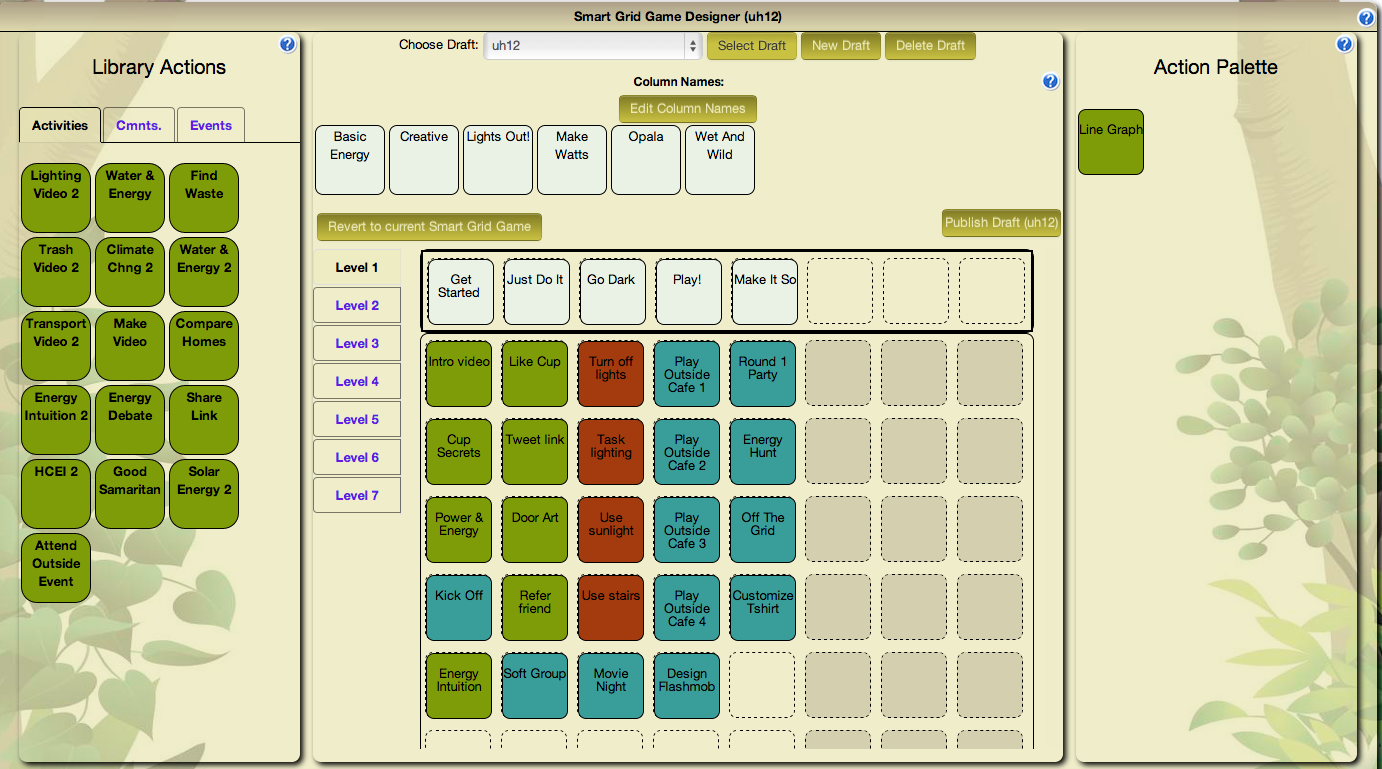
\includegraphics[width=0.9\columnwidth]{smartgrid-game-designer.eps}
  \caption{\em Smart Grid Game Designer widget}
  \label{fig:game-designer}
\end{figure}

The Designer Widget has three columns, Library Actions, Designer Grid, and Palette. 

The Library Actions Column holds a library of Activities, Commitments, and Events. The Library is a reusable set of actions for a sustainability serious game. These actions are divided into three tabs, Activities, Commitments, Events. They are generic actions without any dates or locations associated with them. You can drag these library actions into the Designer Grid. If the Action is an Event you will be asked to provide the event date and location. After the action is dragged into the grid, you can override any of the attributes of the action to be tailored to the need of a specific instance of the serious game challenge.
 
The grid that the Smart Grid Game Designer creates is called ``draft''. Designers can adjust the Designer Grid, adding or removing actions, columns and levels and players will not see the changes until they are published. Multiple drafts can be created by saving the current grid to a different name. Multiple grids allow human game designers to explore different layouts and paths through the Smart Grid Game. Once the designer is satisfied with the draft grid, he can click the ``publish draft'' button to update the live Smart Grid Game that players will see.

The Smart Grid Game Designer also includes a Grid Consistency Checker (GCC) Tool. Because the complexity of grid, especially the interdependency (specified by the predicates) of the grid actions, a draft grid often contains errors and inconsistency. The GCC will be automatically run when the ``publish the draft'' button is pressed and display all the potential errors in the grid. Users should modify the draft to fix any errors found by GCC in order to successfully publish to the live smart grid game. 

Figure \ref{fig:smartgrid-designer-gcc-settings} shows a list of items that checked by the GCC tool. 

\begin{figure}[!ht]
  \center
  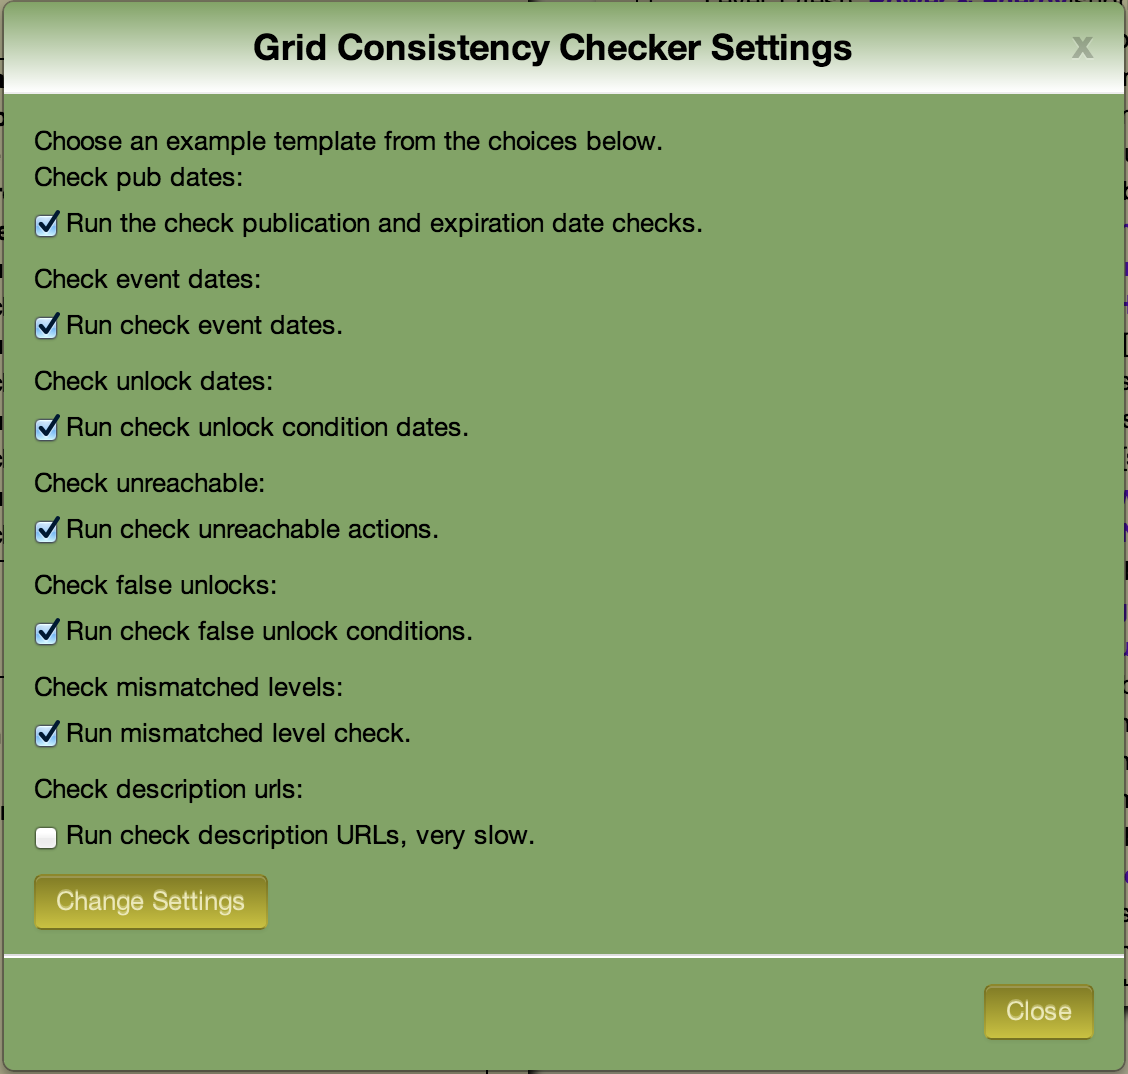
\includegraphics[width=0.6\columnwidth]{smartgrid-designer-gcc-settings.eps}
  \caption{\em Grid Consistency Checker Widget}
  \label{fig:smartgrid-designer-gcc-settings}
\end{figure}

Figure \ref{fig:smartgrid-designer-dependency} shows the action dependency tree that is inspected by the GCC tool. 

 \begin{figure}[!ht]
  \center
  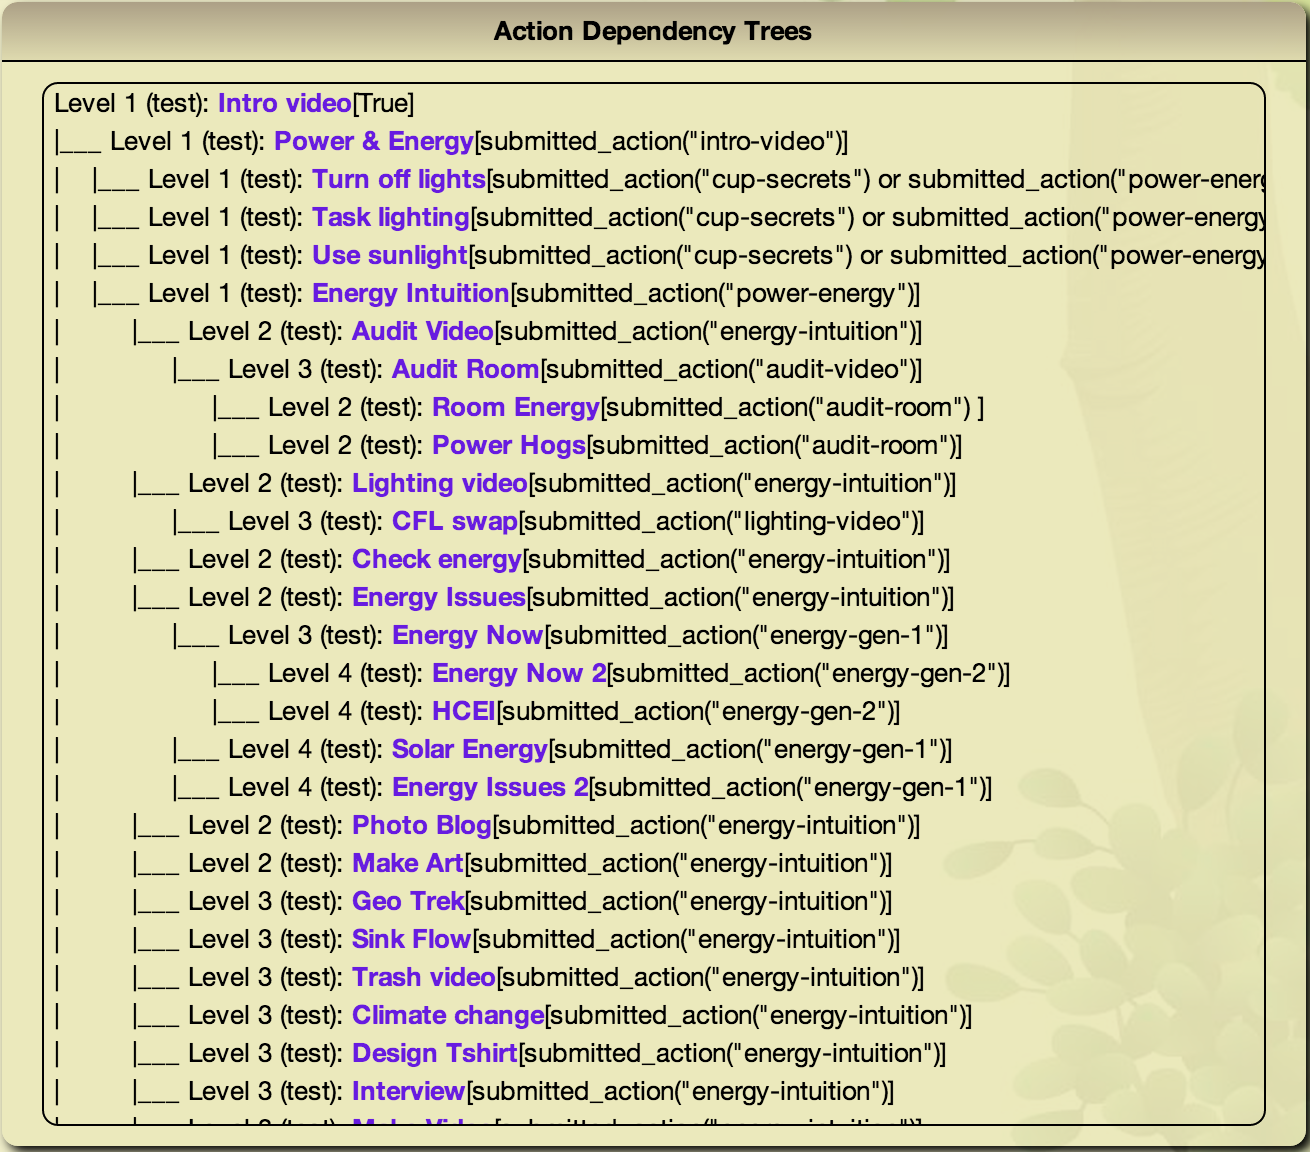
\includegraphics[width=0.6\columnwidth]{smartgrid-designer-dependency.eps}
  \caption{\em Action Dependency Tree}
  \label{fig:smartgrid-designer-dependency}
\end{figure}

\clearpage

\subsubsection{Top Score Game}

The Top Score Game enables you to design a challenge in which prizes are awarded to individuals and teams who earn the most points during the challenge (and/or each round in a challenge). It also enables you to award prizes to the teams that conserved the most energy (or some other resource such as water) during the challenge (and/or each round in the challenge).

The Top Score Game includes both a Leaderboard widget (Figure \ref{fig:topscore-game-scoreboard}) that shows the top players/team in contention for each round, and a Prizes widget (Figure \ref{fig:topscore-game-prize}) that shows the prizes for for each round and the current team/individual in line to win them.

\begin{figure}[!ht]
  \center
  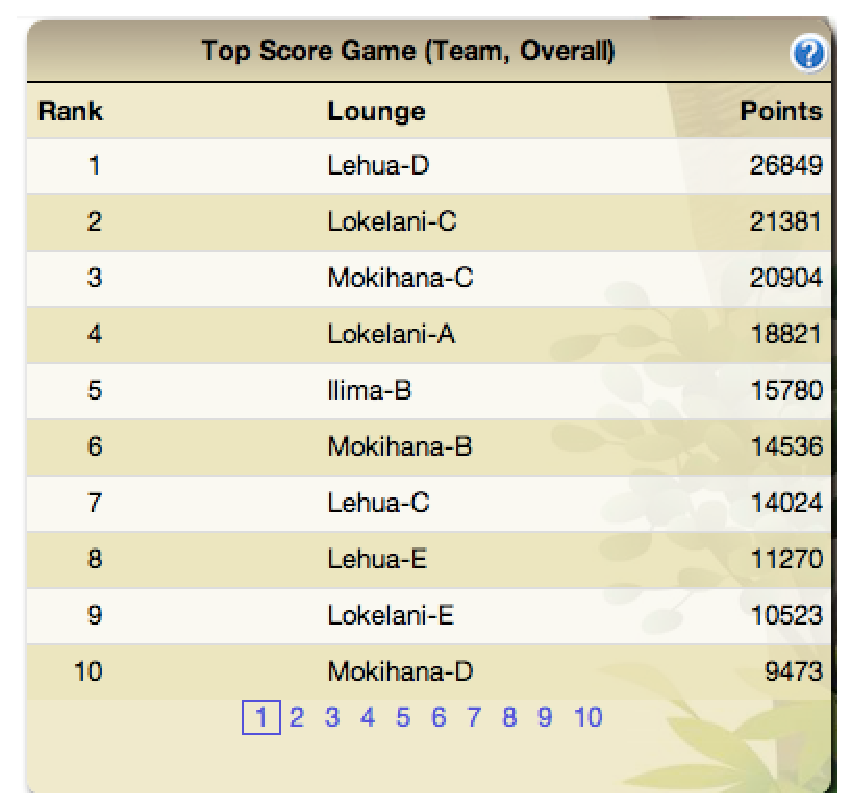
\includegraphics[width=0.55\columnwidth]{topscore-game-scoreboard.eps}
  \caption{\em TopScore Game Scoreboard}
  \label{fig:topscore-game-scoreboard}
\end{figure}

\begin{figure}[!ht]
  \center
  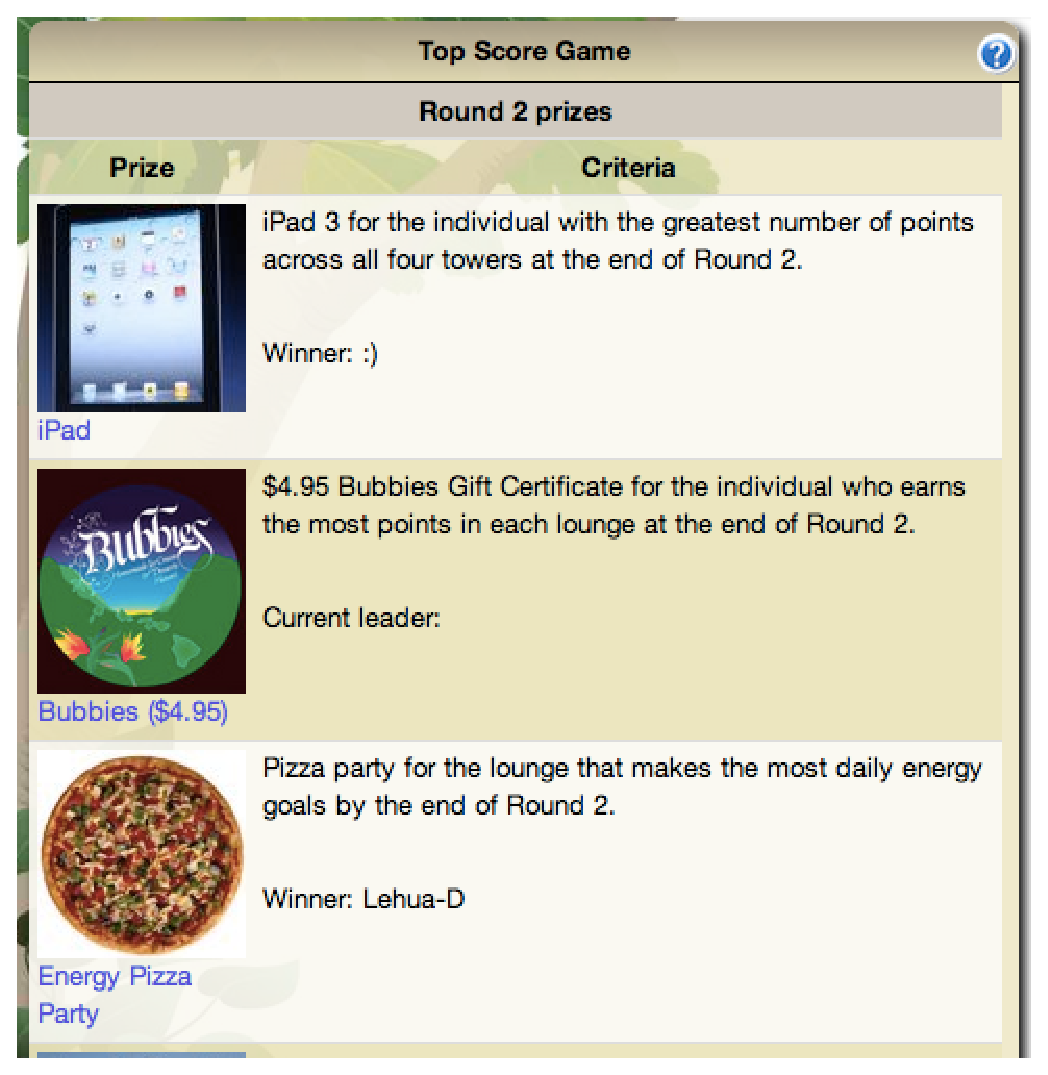
\includegraphics[width=0.6\columnwidth]{topscore-game-prize.eps}
  \caption{\em TopScore Game Prizes}
  \label{fig:topscore-game-prize}
\end{figure}

Designers can configure the prizes for a particular challenge by using TopScore Game configuration on the ``Settings'' page. Figure \ref{fig:topscore-game-change} shows the interface to specify a prize for the challenge.

\begin{figure}[!ht]
  \center
  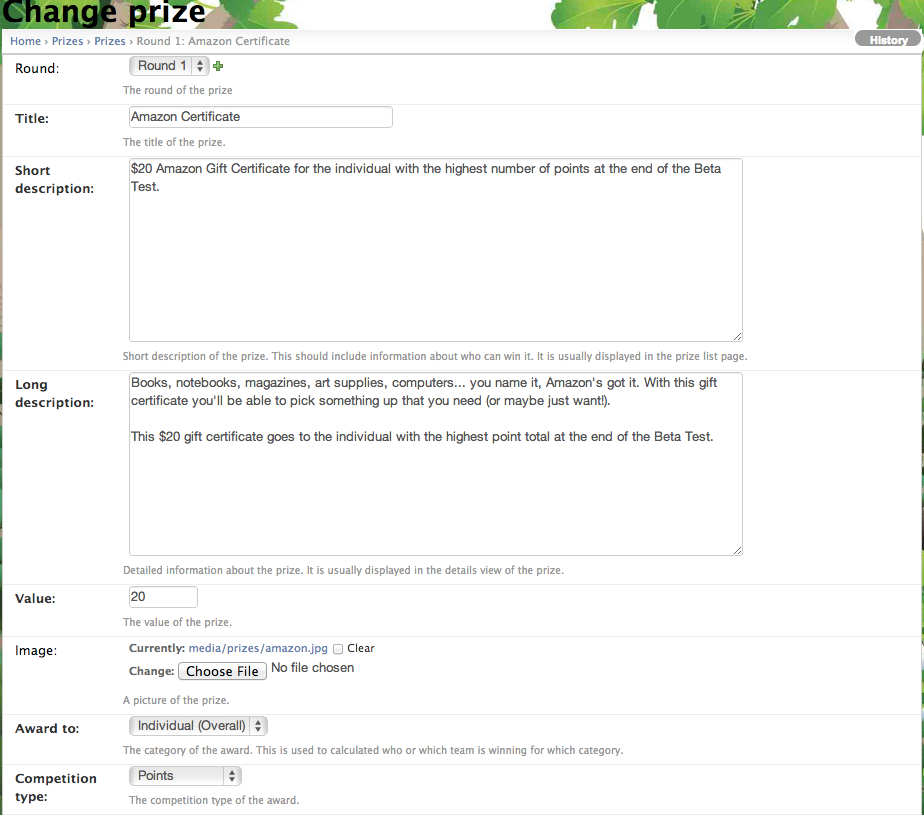
\includegraphics[width=0.85\columnwidth]{topscore-game-change.eps}
  \caption{\em Specifying a TopScore Game Prize}
  \label{fig:topscore-game-change}
\end{figure}

\clearpage

\subsubsection{Raffle Game}

The Raffle Game was designed to solve the problem of incentivizing players who cannot hope to be a top competitor in the Challenge. When several hundred players are competing, only a handful have a realistic chance to be the top scorers for a round. Once a player knows they cannot beat all of the other players, there can be an urge to simply give up.

The Raffle Game is designed to enable all players to have a chance to win a wide variety of prizes, where their odds of winning increase based upon the number points they have earned in the game; thus incentivize participation from all individuals, even those who are not in the running for a top prize. Figure \ref{fig:RaffleGame} shows an example of the Raffle Game.

\begin{figure}[!ht]
  \center
  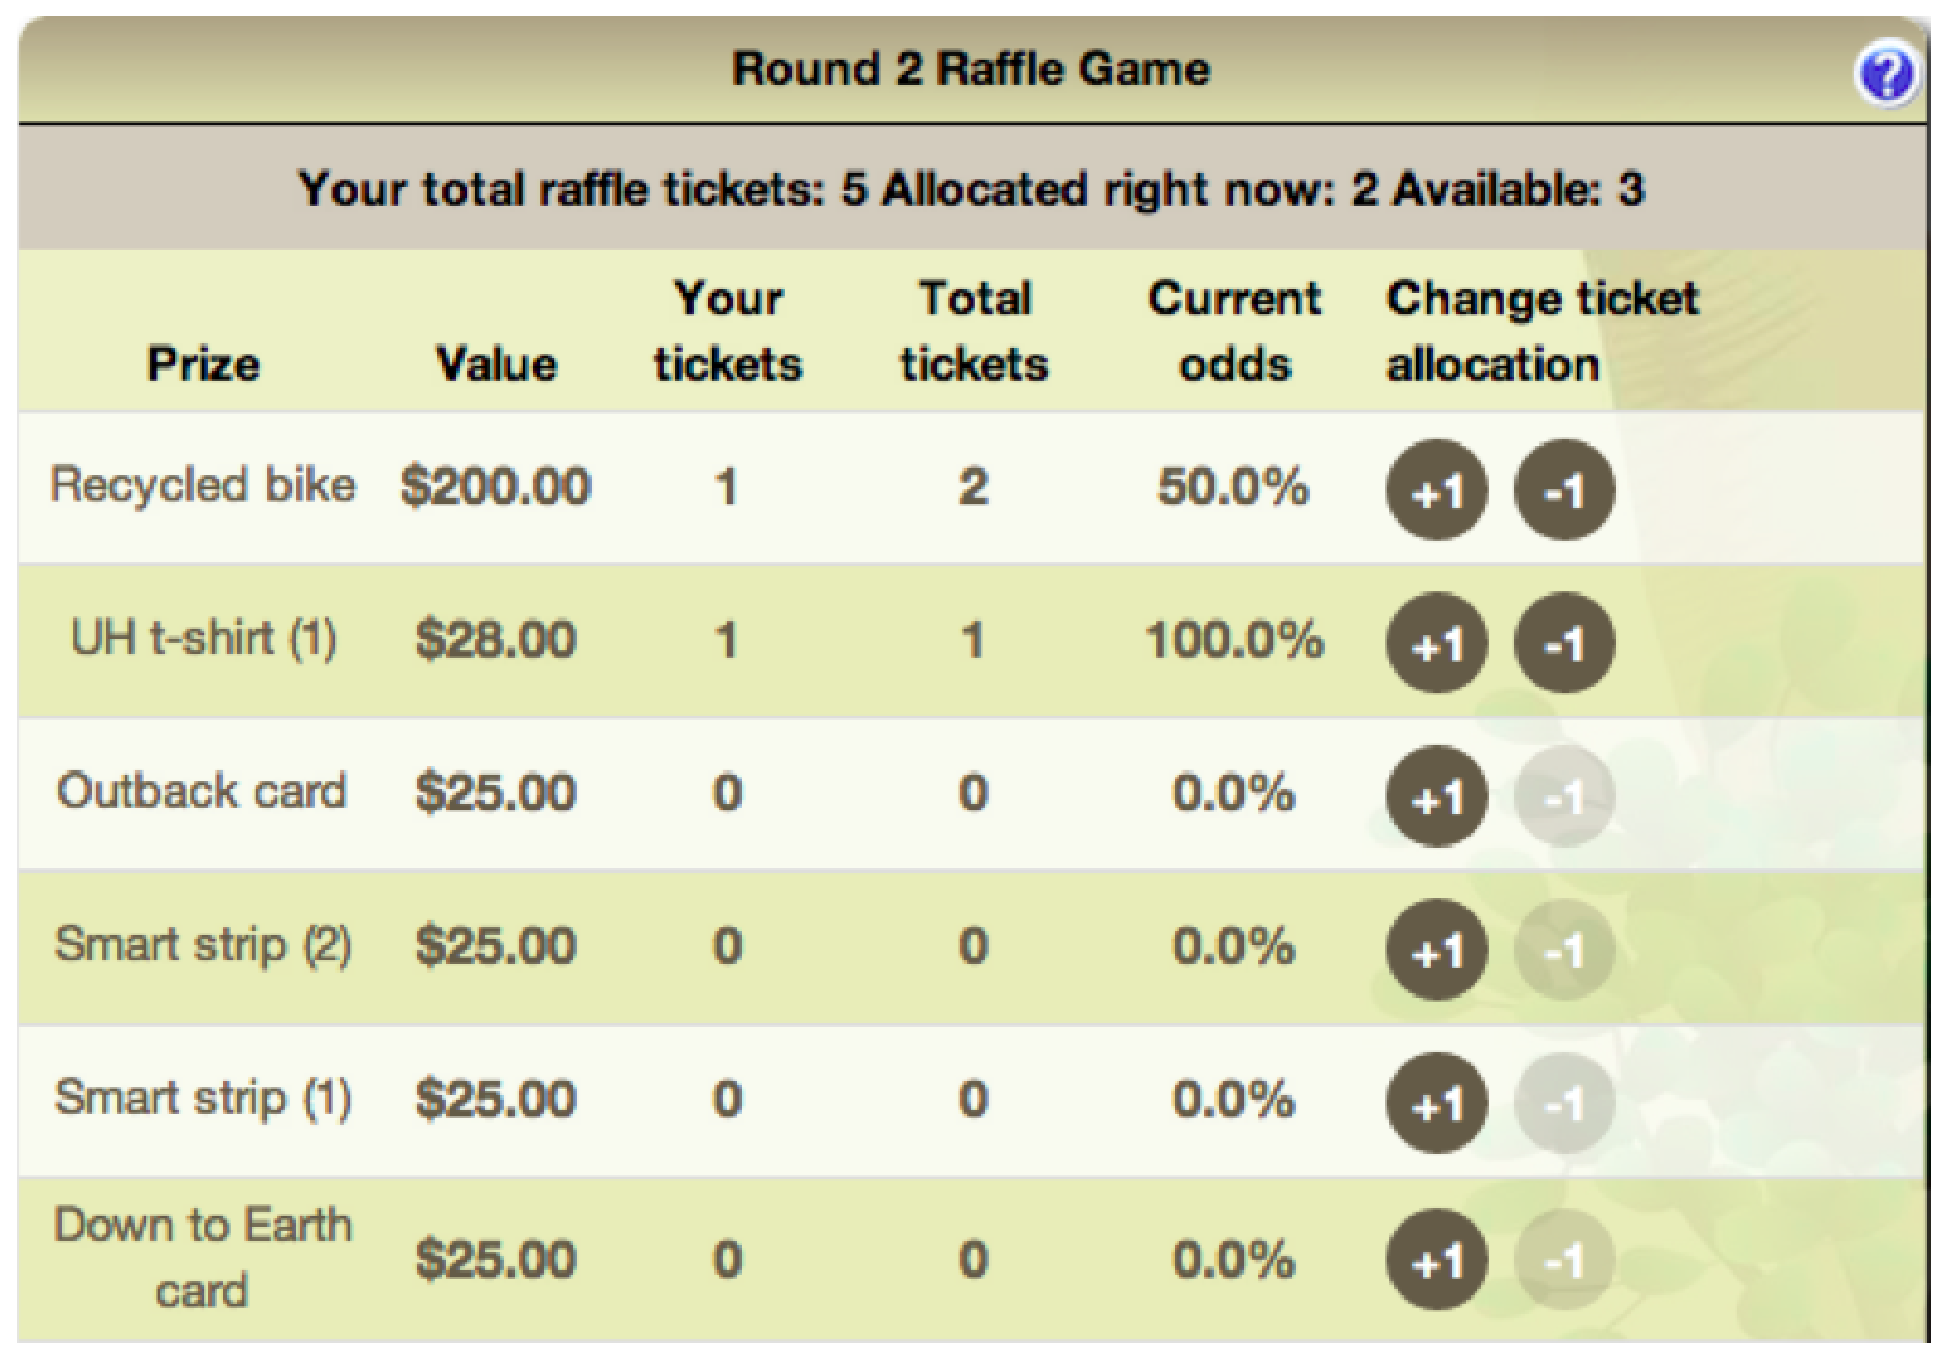
\includegraphics[width=0.6\columnwidth]{raffle-small.eps}
  \caption{\em Raffle Game widget}
  \label{fig:RaffleGame}
\end{figure}

Each round of the competition has its own set of raffle prizes and any unused raffle tickets carry over to the next round. Raffle tickets are independent from a player's score, and allocating a raffle ticket does not affect their rank. The system provides random selection of the winner of each raffle item at the end of a round.

The Raffle Game works in the following way. For every 25 points (by default) that a player earns, they receive one virtual raffle ticket. Players can dynamically allocate their tickets to any raffle prizes they are interested in at any time, up to the end of the raffle. Each round of the competition has its own set of raffle prizes and any unused raffle tickets carry over to the next round. Raffle tickets are independent from a player's score; allocating a raffle ticket does not affect their rank.

As the screen image above shows, each player can see in real-time how many Raffle Game Tickets they have earned, which prizes they have allocated them to, and the resulting percentage chance they have of winning based upon the tickets allocated by others to that same prize. Of course, these odds can change on a moment-to-moment basis as players allocated and deallocated tickets.

The Raffle Game, in addition to providing an incentive for the non-top players to earn points, also creates an incentive for players to come back to the site on a regular basis to see the updated odds associated with their choices.

Designers can configure the raffle prizes for a particular challenge by using Raffle Game Configuration link on the ``Settings'' page. Figure \ref{fig:raffle-game-change} shows the interface to specify a prize for the challenge.

\begin{figure}[!ht]
  \center
  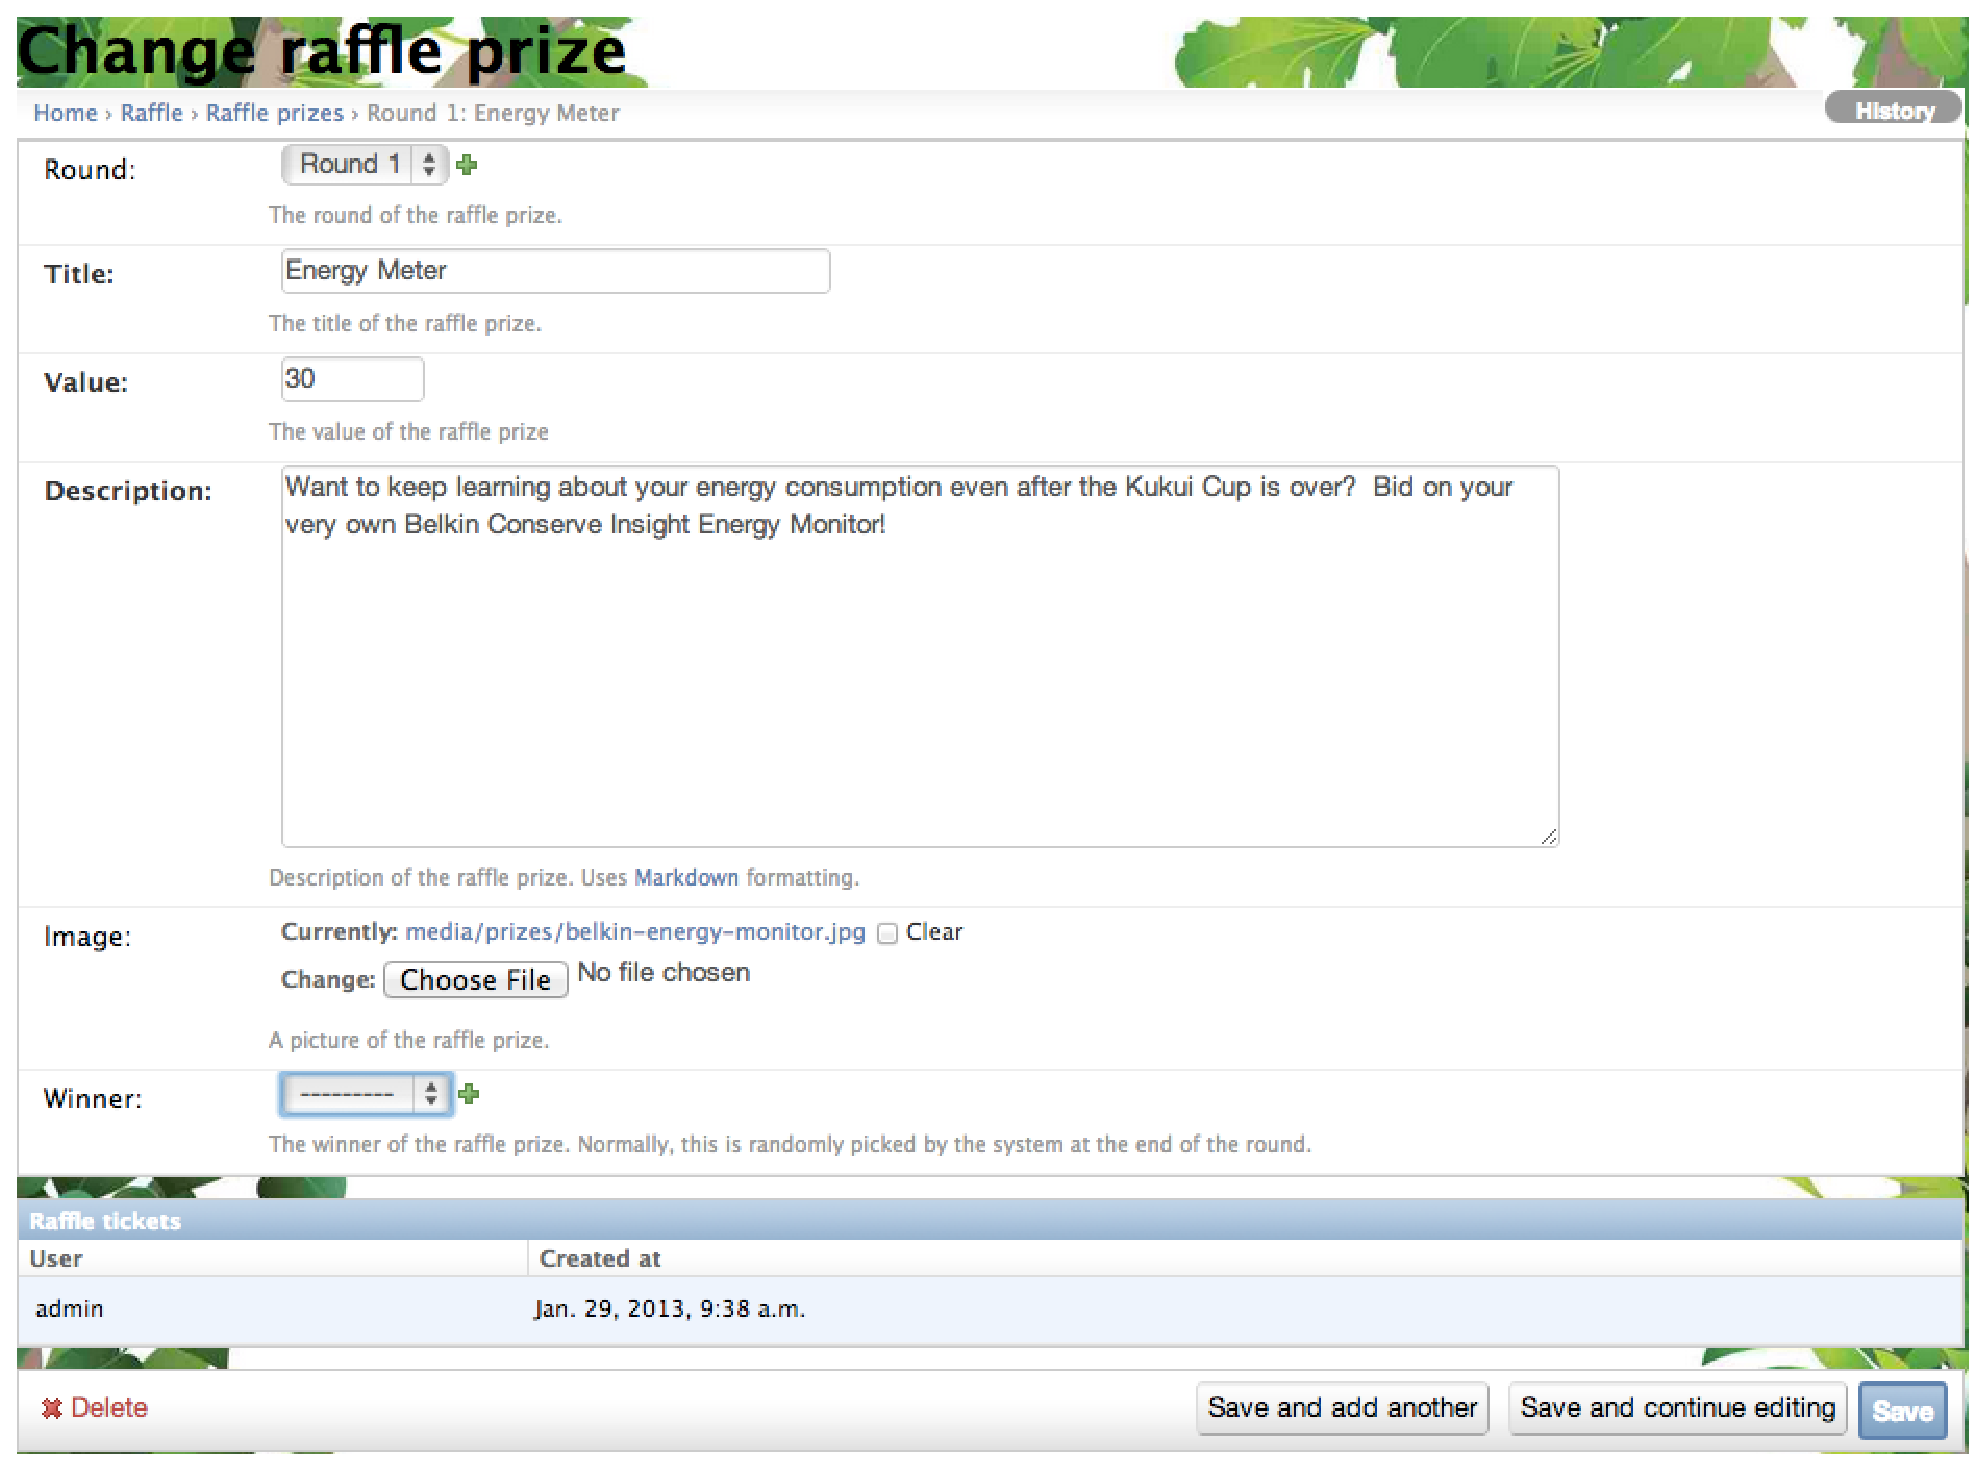
\includegraphics[width=0.8\columnwidth]{raffle-game-change.eps}
  \caption{\em Specifying a Raffle Game Prize}
  \label{fig:raffle-game-change}
\end{figure}

The ``Winner'' of the raffle prize is randomly picked by the system at the end of the round. At the end of the page, you can also see a list of users that allocated raffle tickets for this raffle prize.

\clearpage

\subsubsection{Participation Game}

One of the design constraints of the sustainability serious game such as the Kukui Cup challenge is that, the players associated with each team in a challenge must be specified in advance of a challenge. Thus, as the challenge runs, it is possible to know exactly what percentage of each team's players are actively playing the game (in the sense that they have logged in at least once).

The Participation Game is designed to incentivize active players on a team to recruit other members of their team to login and try the game. It does this by providing extra points to all active players on a team when the percentage participation by that team reaches certain thresholds (currently 50, 75, and 100).

The current percentage participation by a player's team is shown in a scoreboard, as shown in the Figure \ref{fig:participation-game-scoreboard}. Players will receive an in-game notification whenever they reach a threshold participation where points are awarded.

\begin{figure}[!ht]
  \center
  
\includegraphics[width=0.55\columnwidth]{participation-game-scoreboard.eps}
  \caption{\em Participation Game Scoreboard}
  \label{fig:participation-game-scoreboard}
\end{figure}

To configure the participation game, click on the ``Participation Settings'' link in the Participation Game Admin widget on the ``settings'' admin page. Figure \ref{fig:participation-game-scoreboard} shows the settings of the participation game. You can change the points to award for each participation percentage. Currently, the percentages (50, 75, and 100) are hardwired into the system.

\begin{figure}[!ht]
  \center
  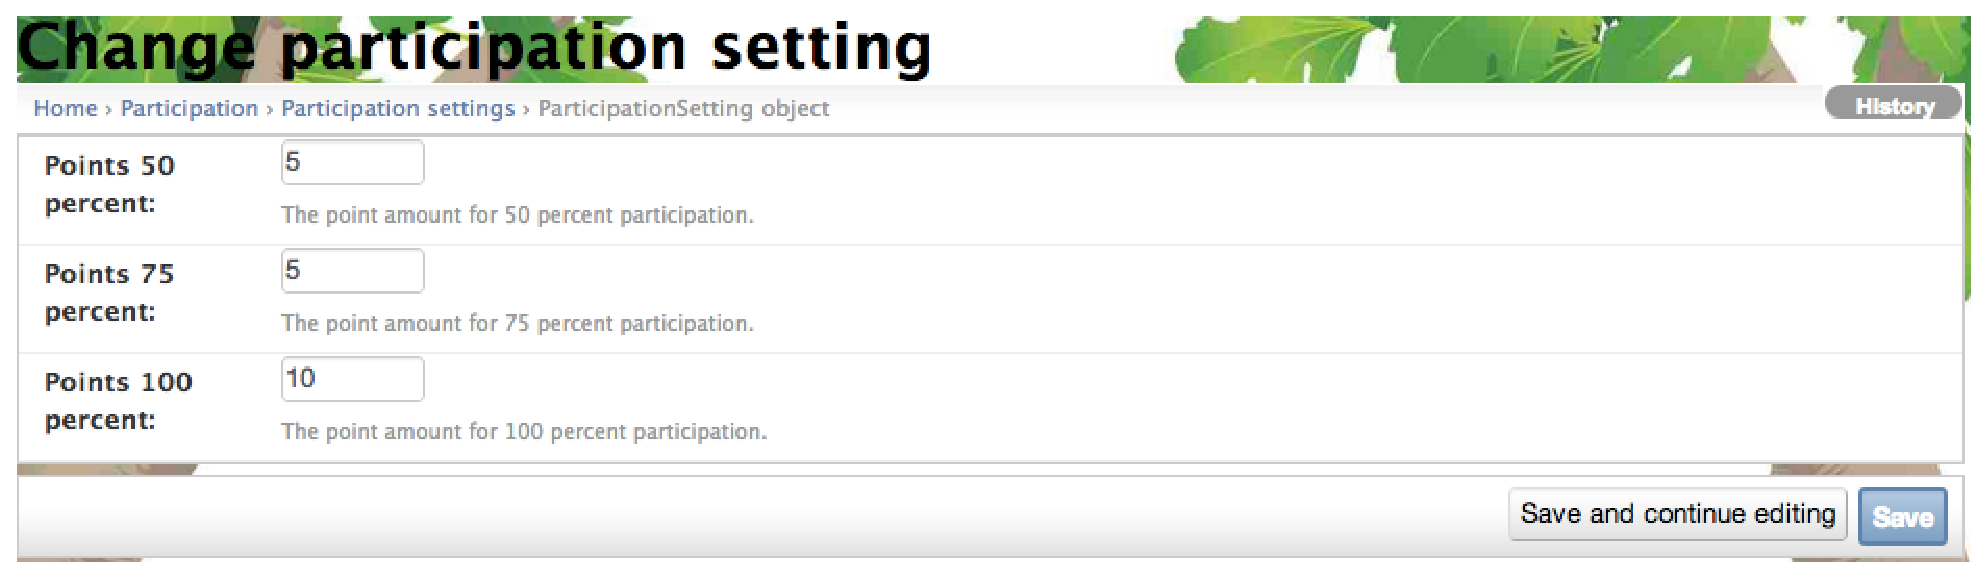
\includegraphics[width=0.8\columnwidth]{participation-game-change.eps}
  \caption{\em Specifying a participation Game Settings}
  \label{fig:participation-game-change}
\end{figure}

\subsubsection{Quest Game Mechanics}
One fundamental challenge faced by any game is: how do players learn how to play it? This is generally known as the on-boarding problem. Makahiki provides a configurable ``Quest Engine'', that enables the definition of quests and the dependencies among them. That enables site developers to create a kind of structured, proactive user guide for the system. Instead of stumbling on a random playable feature of the game, players learn about the capabilities of the site by performing discrete sequences of actions, call ``Quests''. 

Quests are made available to the player in a collapsible/expandable window right below the navigation bar. The set of Quests shown to a player can depend upon their game state, so that ``simple'' Quests can be presented initially and more ``complicated'' Quests presented as the player gains in expertise. Quests generally guide the player through the various workflows of the Challenge, such as completing a task, signing up for an event, or allocating a raffle ticket.

The system shows a maximum of three Quests at a time. Figure \ref{fig:guided-tour-quests} shows an example of an expanded quest and its content. Once the player accepts the quest, and follows the instruction to complete the quest, the notification dialog box will appear to the player indicating the accepted quest had been completed. A new potentially harder quest will appear in the quest window replacing the completed quest.

\begin{figure}[!ht]
  \center
  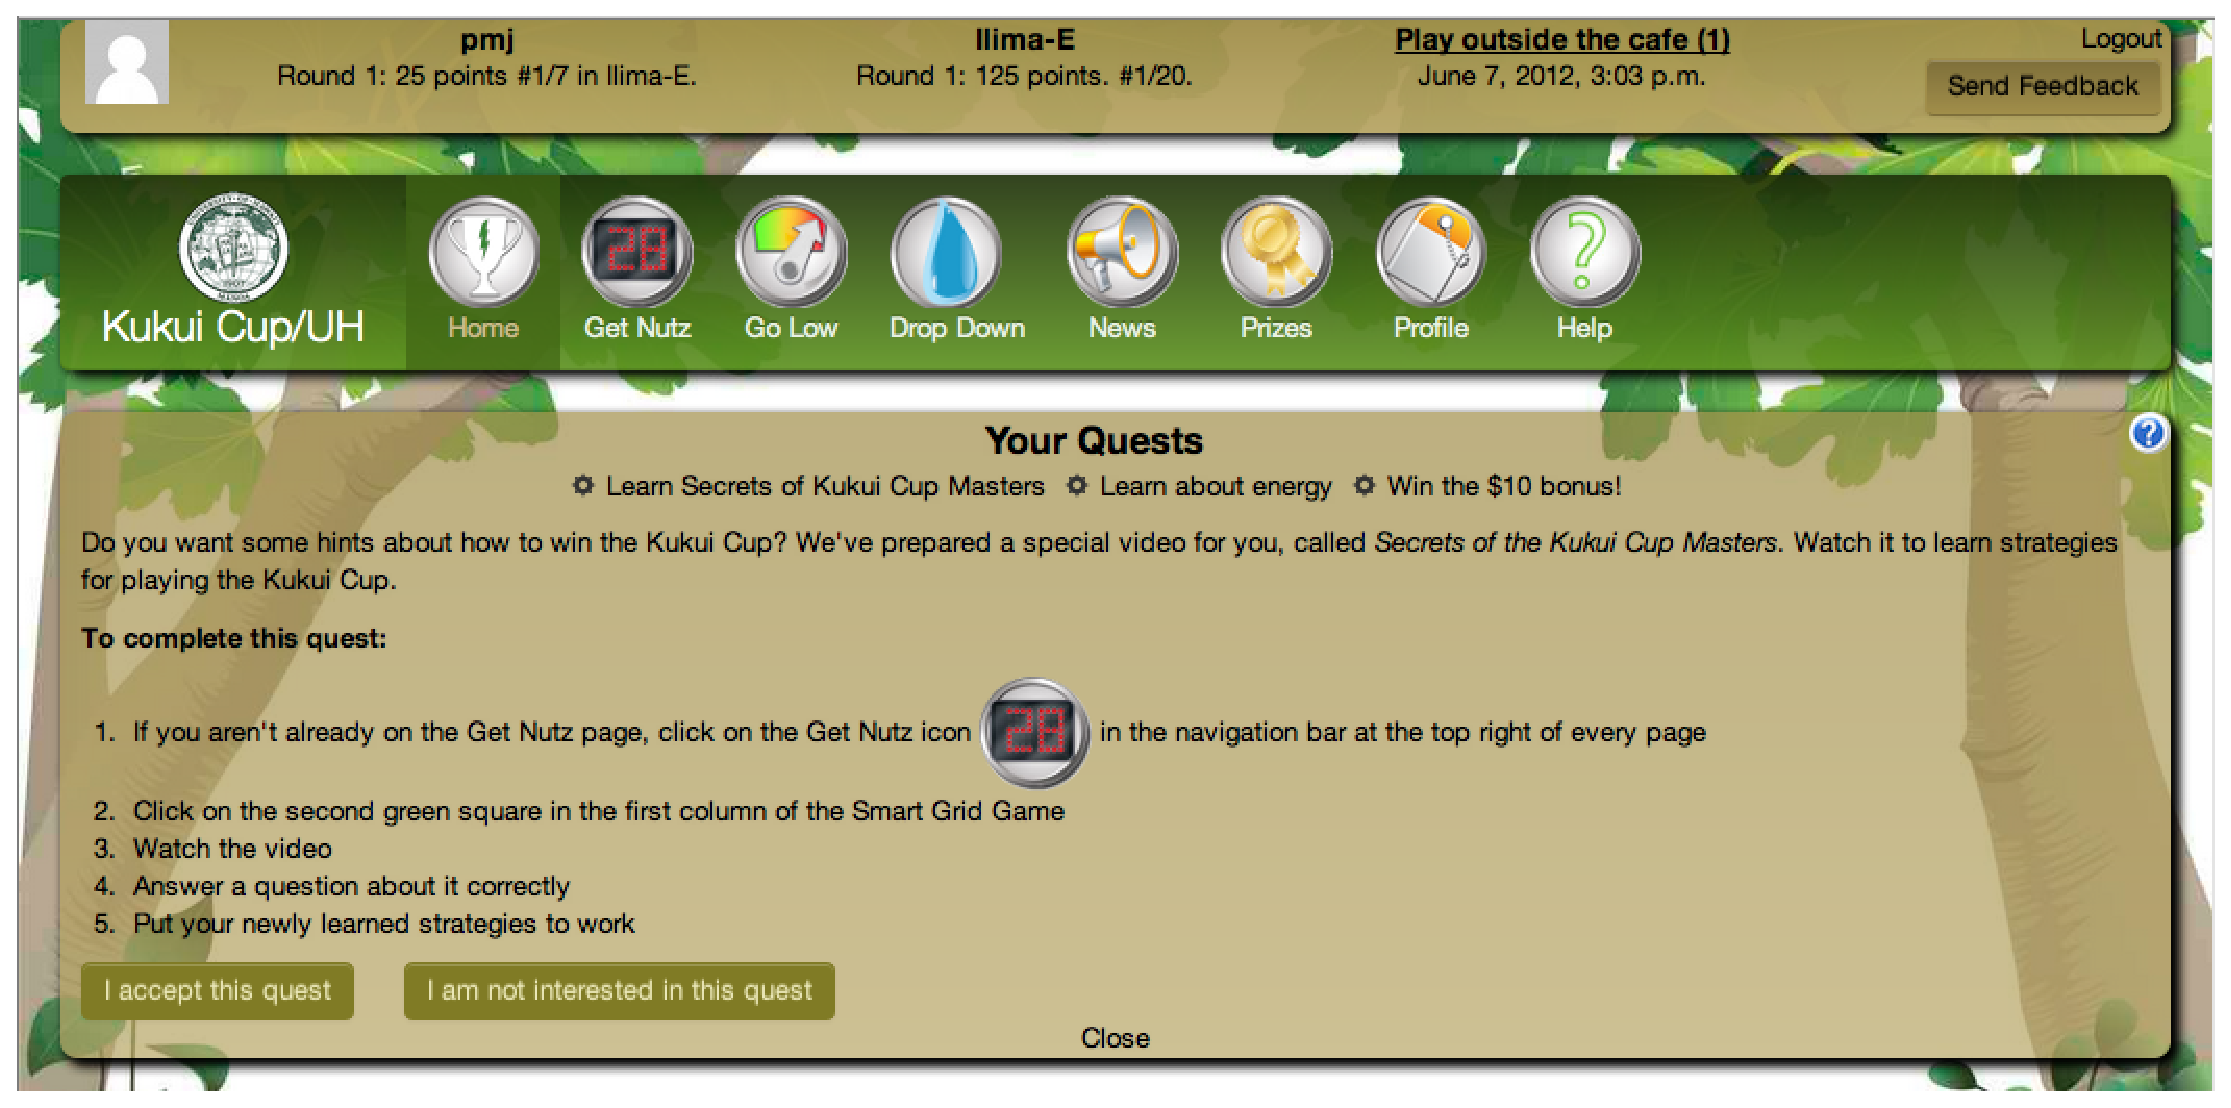
\includegraphics[width=0.9\columnwidth]{guided-tour-quests.eps}
  \caption{\em Quest Game Mechanics}
  \label{fig:guided-tour-quests}
\end{figure}

Quests are created by the administrator prior to the Challenge. Administrators have the option of specifying a set of predicates to determine when the player could be shown a Quest and when the player has completed the Quest, and it should no longer be shown.

Designers can configure the quests for a particular challenge by using Quest Game Mechanics Configuration link on the ``Settings'' page. Figure \ref{fig:quest-change} shows the interface to specify a quest for the challenge.

\begin{figure}[!ht]
  \center
  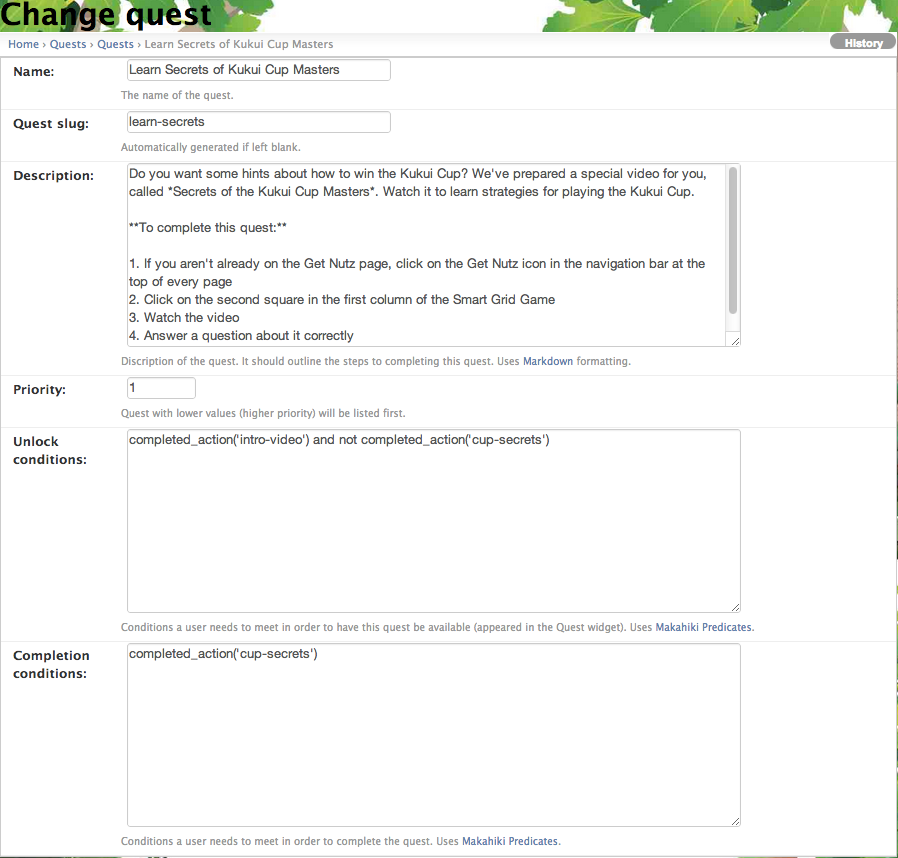
\includegraphics[width=0.9\columnwidth]{quest-change.eps}
  \caption{\em Specifying a Quest Game Mechanics}
  \label{fig:quest-change}
\end{figure}

\clearpage

\subsubsection{Badge Game Mechanics}

Makahiki provides the badge game mechanics to motivate and engage players. The badge mechanics is implemented in a customizable way which game designers could create as many badges as they like. The badge could be triggered by certain award condition, which is defined by the flexible predicative system in Makahiki. 

Badges are a common game mechanic, in which players receive recognition for various accomplishments. Makahiki allows the challenge designer to specify the set of badges available in a challenge, and to define new ones. The challenge designer has the option of making badges worth points. Finally, the designer can use the Makahiki predicate system to award a badge automatically (for example, when a player has completed a Level in the Smart Grid Game), or manually award the badge through administrator action (for example, when a player reports a significant bug in the system).

In many systems, each badge has a custom design, but in Makahiki, we decided that the overhead of providing a custom graphic for each badge outweighed the benefits. Providing a custom graphic also would creates complexity with another feature of Makahiki: the ability to create ``themes'' with different colors. To be consistence with the themes in Makahiki, badges have a common look and feel consisting of a circle and a multi-character ID. Its actual colors are specified by the theme, and can thus vary from theme to theme.

Figure\ref{fig:badge} shows an example of the badges available in the Makahiki system:

\begin{figure}[t!]
  \center
  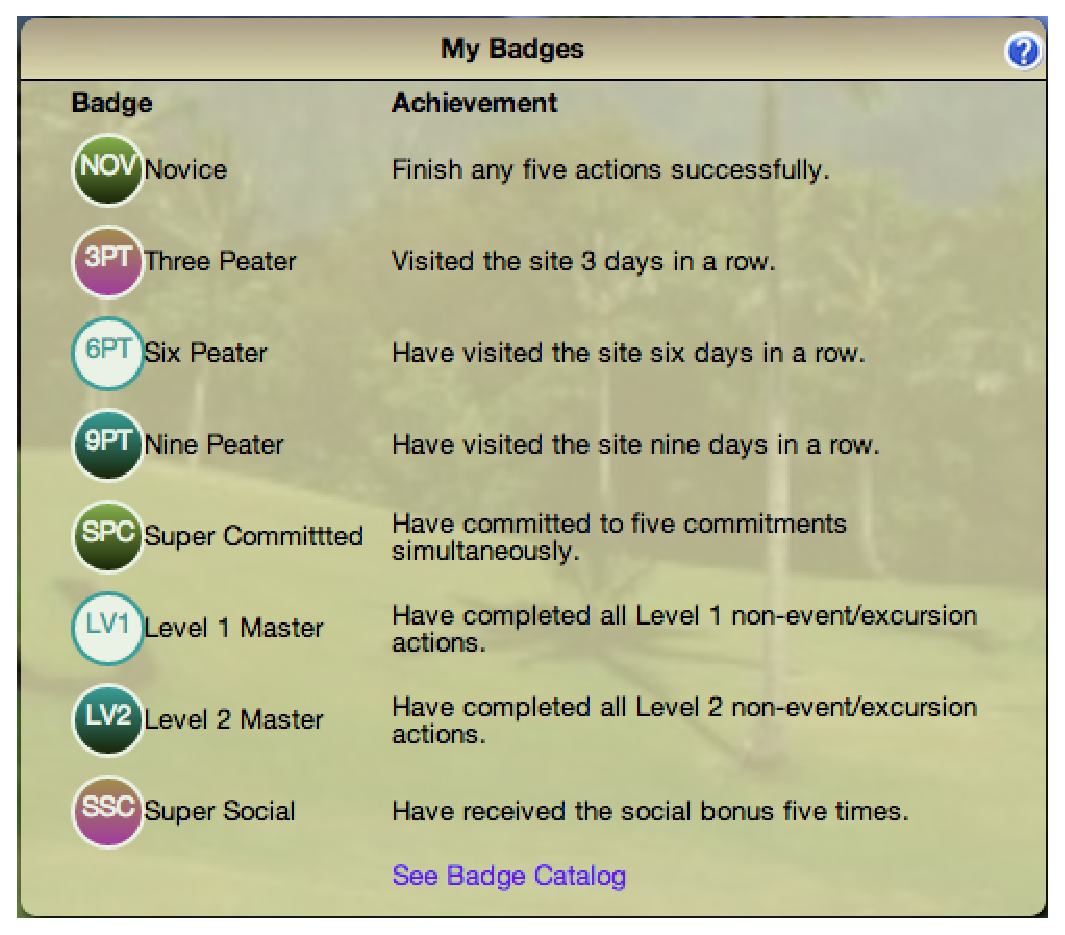
\includegraphics[width=0.6\columnwidth]{badge.eps}
  \caption{Badge widget}
  \label{fig:badge}
\end{figure}

Designers can configure the badges for a particular challenge by using Badge Game Mechanics Configuration link on the ``Settings'' page. Figure \ref{fig:badge-change} shows the interface to specify a badge for the challenge.

\begin{figure}[!ht]
  \center
  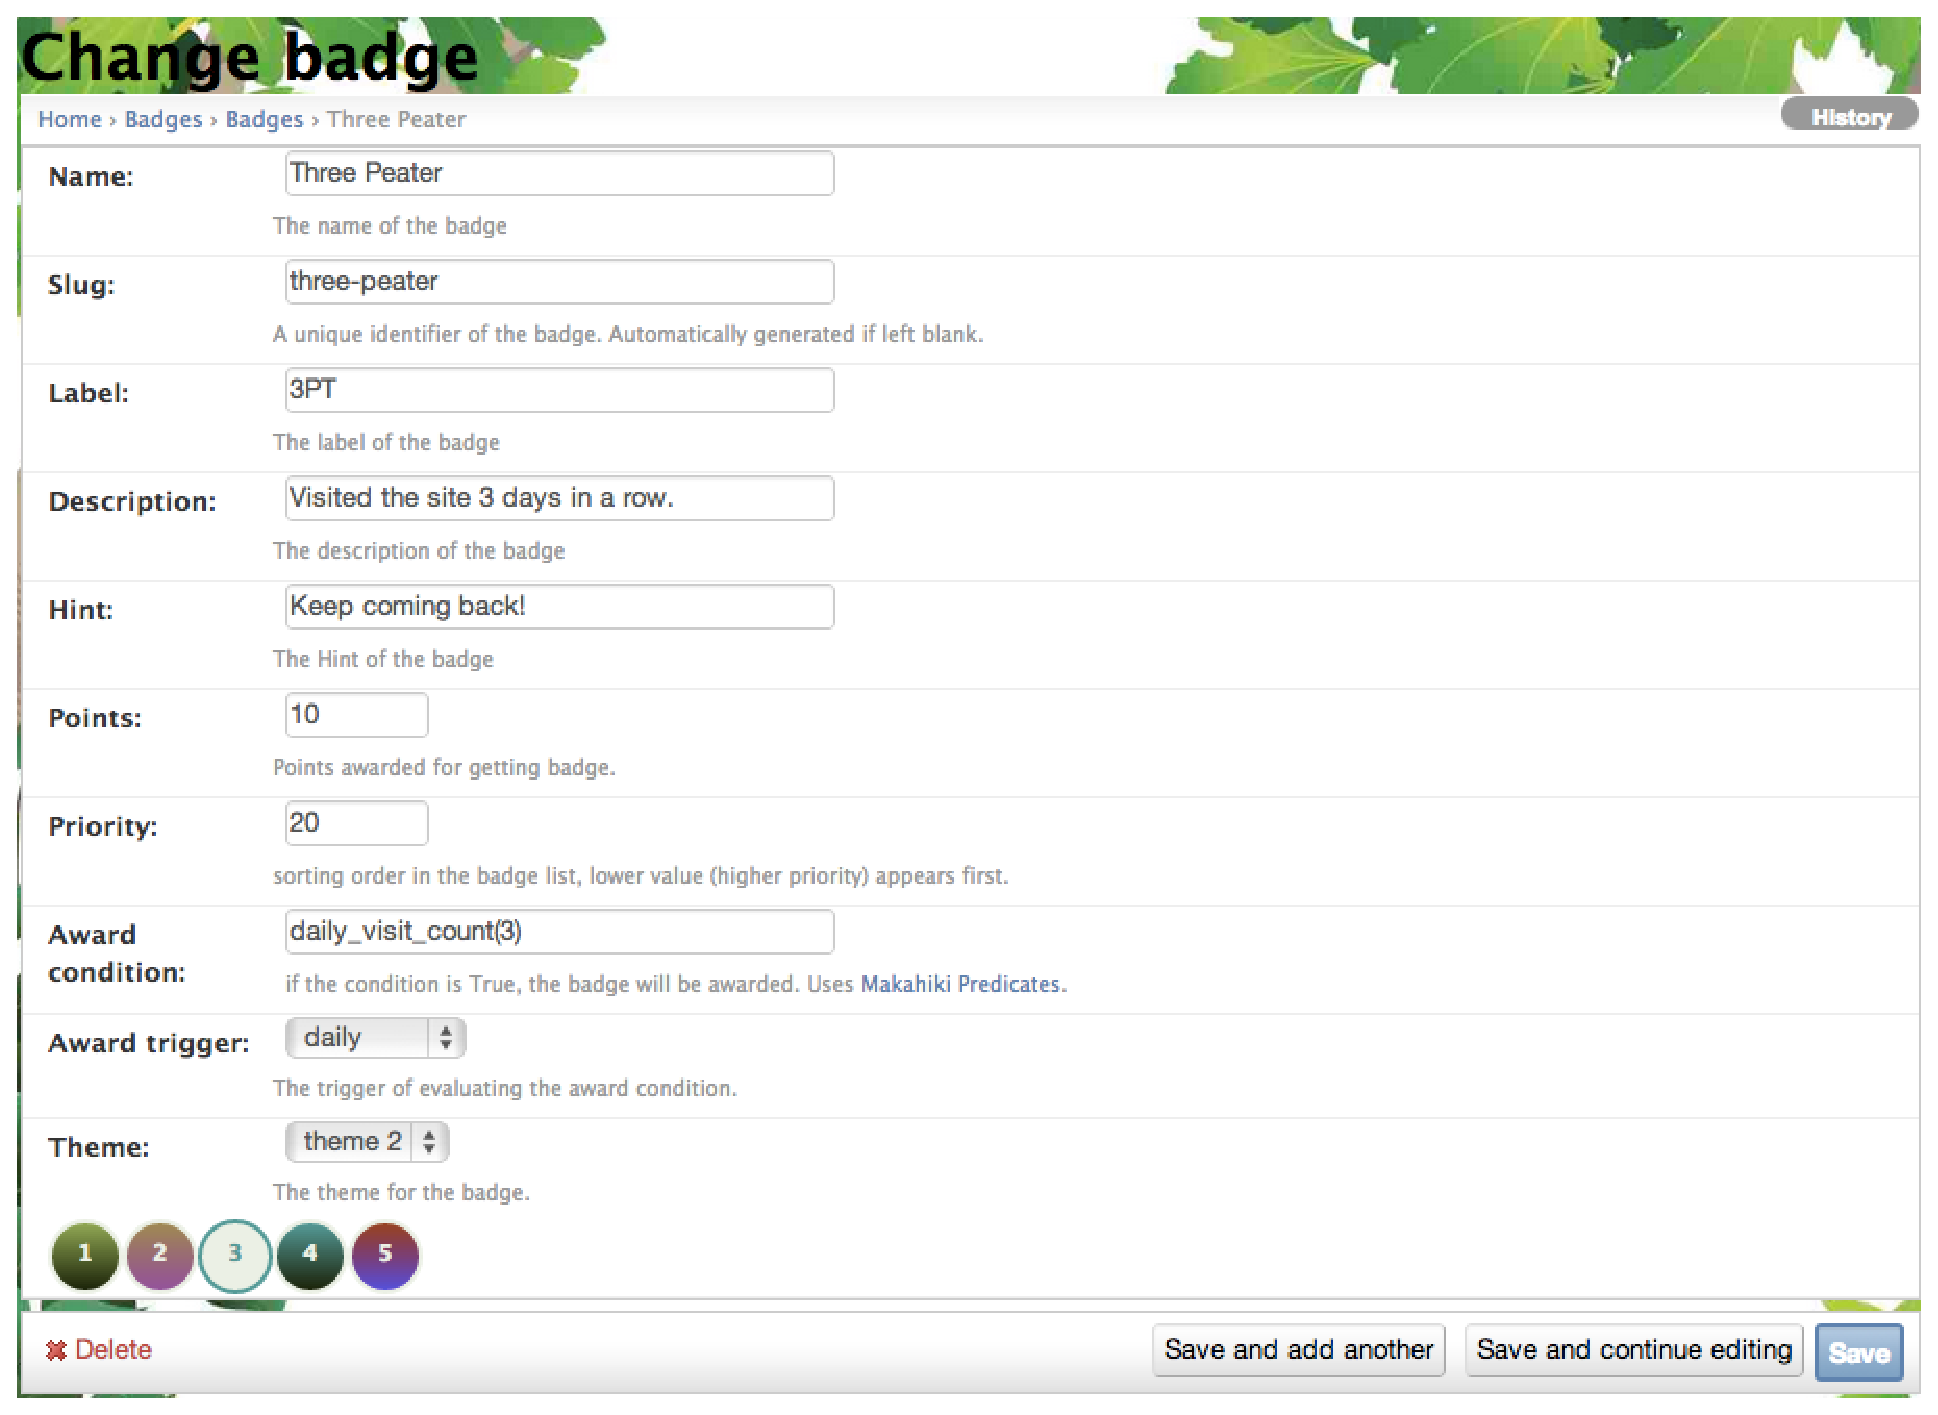
\includegraphics[width=0.8\columnwidth]{badge-change.eps}
  \caption{\em Specifying a Badge Game Mechanics}
  \label{fig:badge-change}
\end{figure}

\clearpage

\subsubsection{Referral Bonuses Game Mechanics}

Similar to social bonus described in the Smart Grid Game above, the Referral Bonus is the game mechanics that help encourage participation by providing additional points to players who participate in activities with other players, and facilitate the entry of new players into an energy challenge.

Players are led through a setup process when logging into Makahiki for the first time. One of the steps in this process is the referral bonus. If a player was referred by another player in the system, they can use this step to input their email address. Once the new player earns a certain number of points in the competition, both players are awarded a referral bonus of a configurable number of points. Typically, going through the setup process gives you 25 points, so setting a point threshold of 30 points encourages the new player to at least complete one additional action in order to get the referral bonus.

When enabled, the referral bonus is implemented as a step in the first login process, as shown in Figure \ref{fig:referral-bonus}.

\begin{figure}[!ht]
  \center
  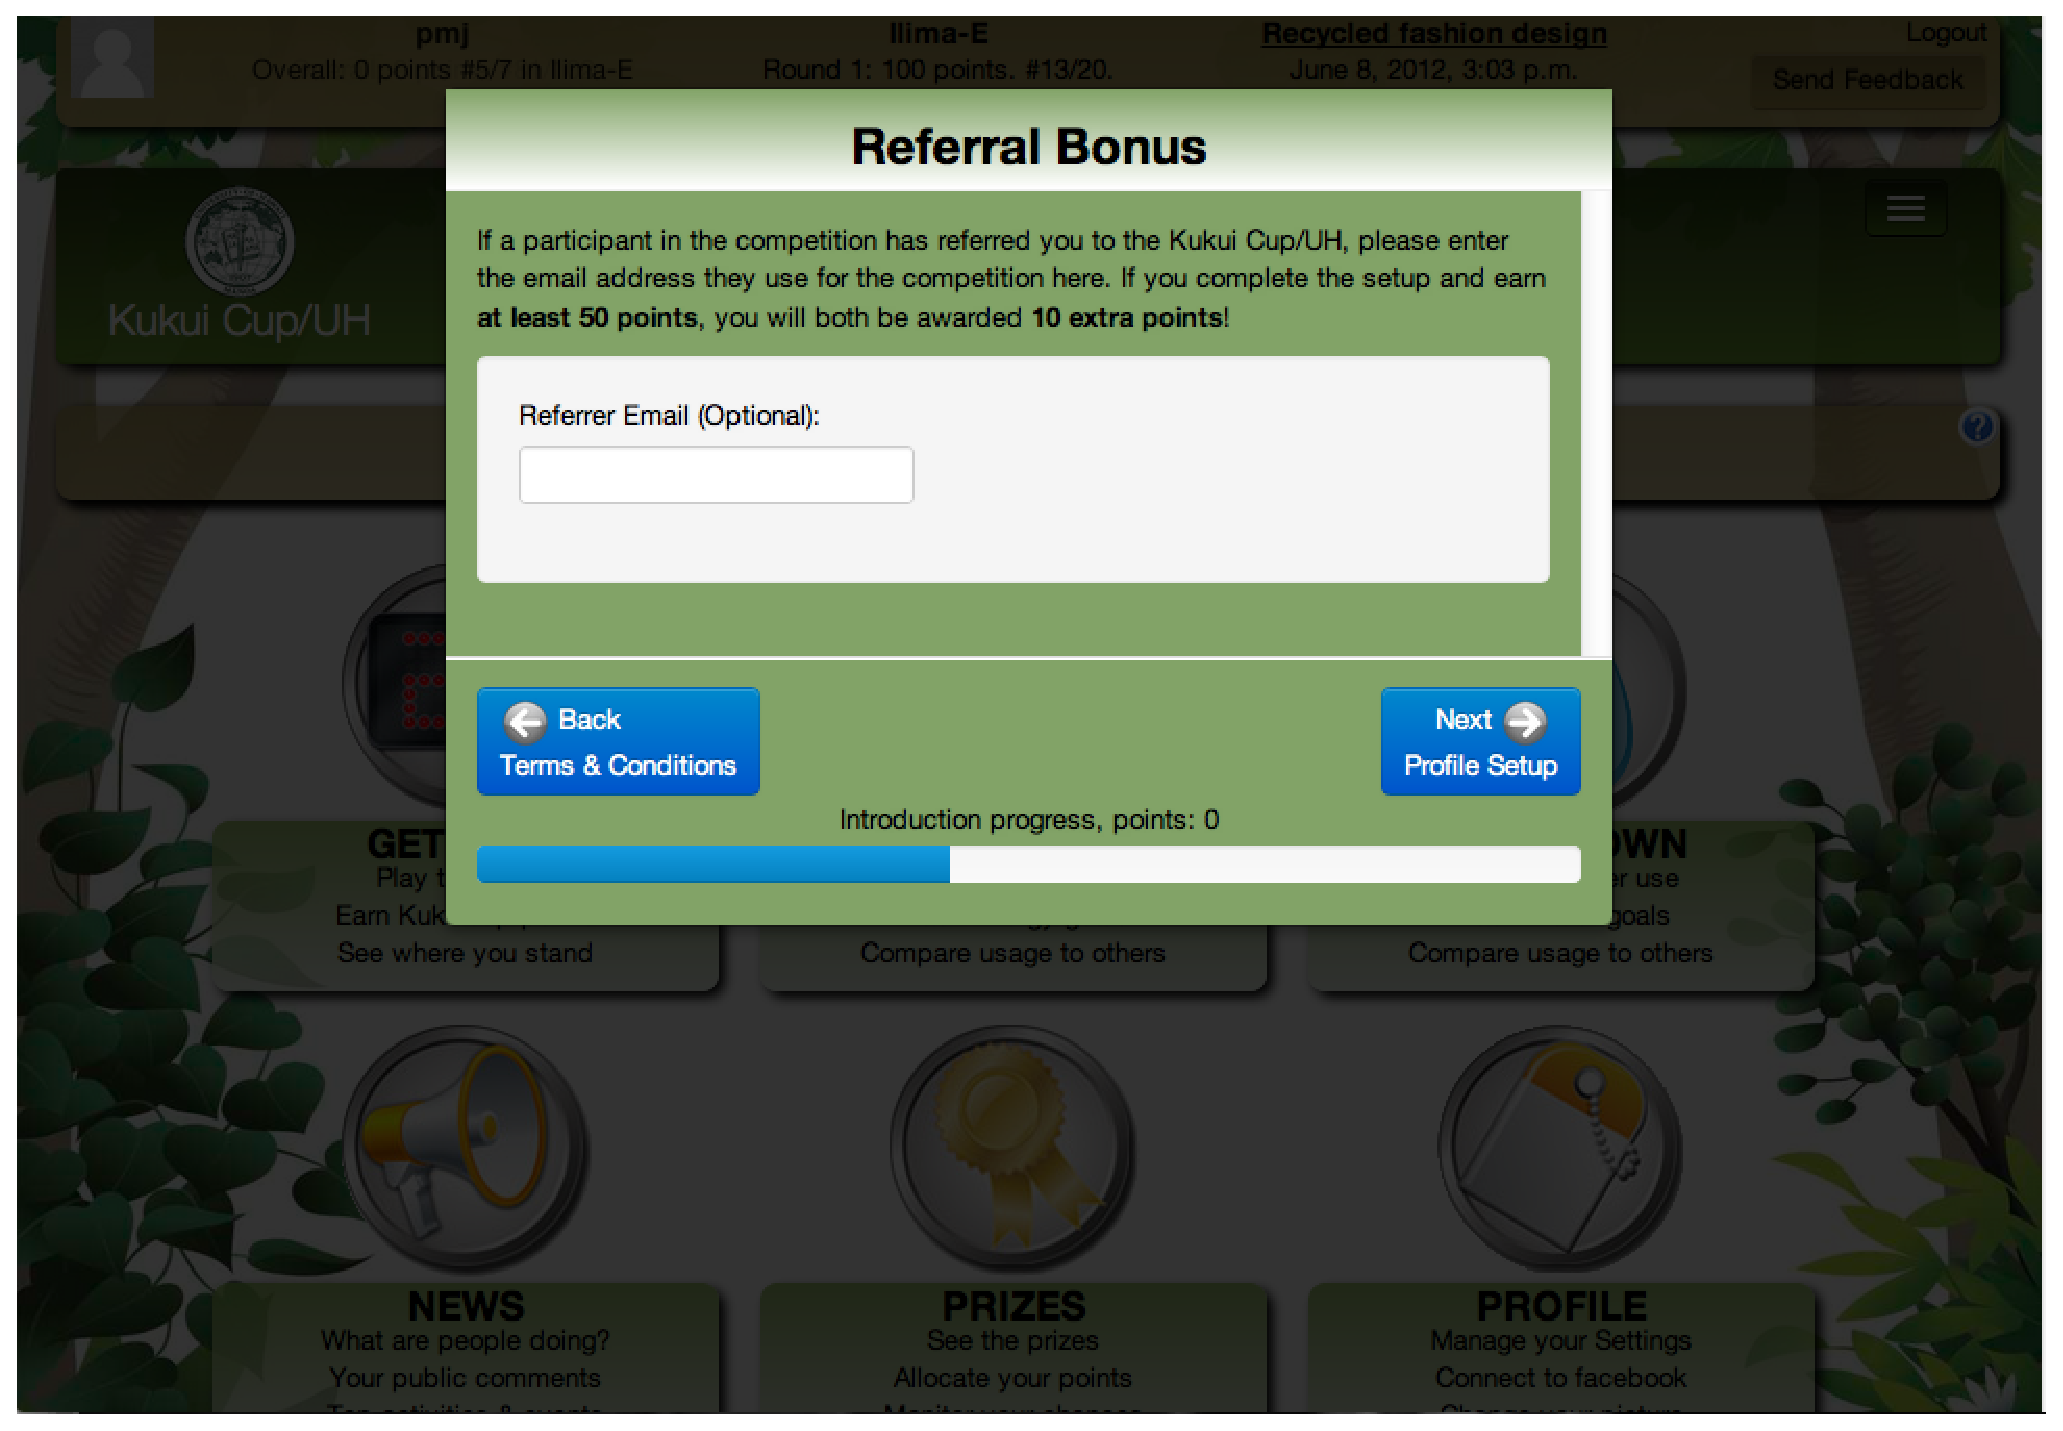
\includegraphics[width=0.85\columnwidth]{referral-bonus.eps}
  \caption{\em Referral Bonus Game Mechanics Widget}
  \label{fig:referral-bonus}
\end{figure}

If the new player was referred to the challenge by another player, they can use this step to input their email address. Once the new player earns 30 points in the competition, both players are awarded a referral bonus of (typically) 10 points. Typically, going through the setup process gives you 25 points, so a threshold of 30 points means the new player has to complete at least one additional task in order to get the referral bonus.

You can disable the referral game mechanics by clicking on the ``Referral Game Mechanics'' link. If referral game mechanics is disabled, then this window is omitted from the first login wizard and players will not be able to get points by referring other players.

The referral bonus also has a ``dynamic bonus'' capability. If enabled, then you can vary the amount of points awarded depending upon the participation level of the team associated with the new player. This incentivizes players to not just recruit new players for their own team, but to also recruit players for other teams who might not have much participation.

If the referral game mechanics is enabled, which is true by default, you will see the ``Referral settings'' link in the Game Admin widget. After clicking on the ``Referral Settings'' link , You will see the overview of the referral settings, clicking on any of the links, will bring you to a page (Figure \ref{fig:referral-change} to change the settings:

\begin{figure}[!ht]
  \center
  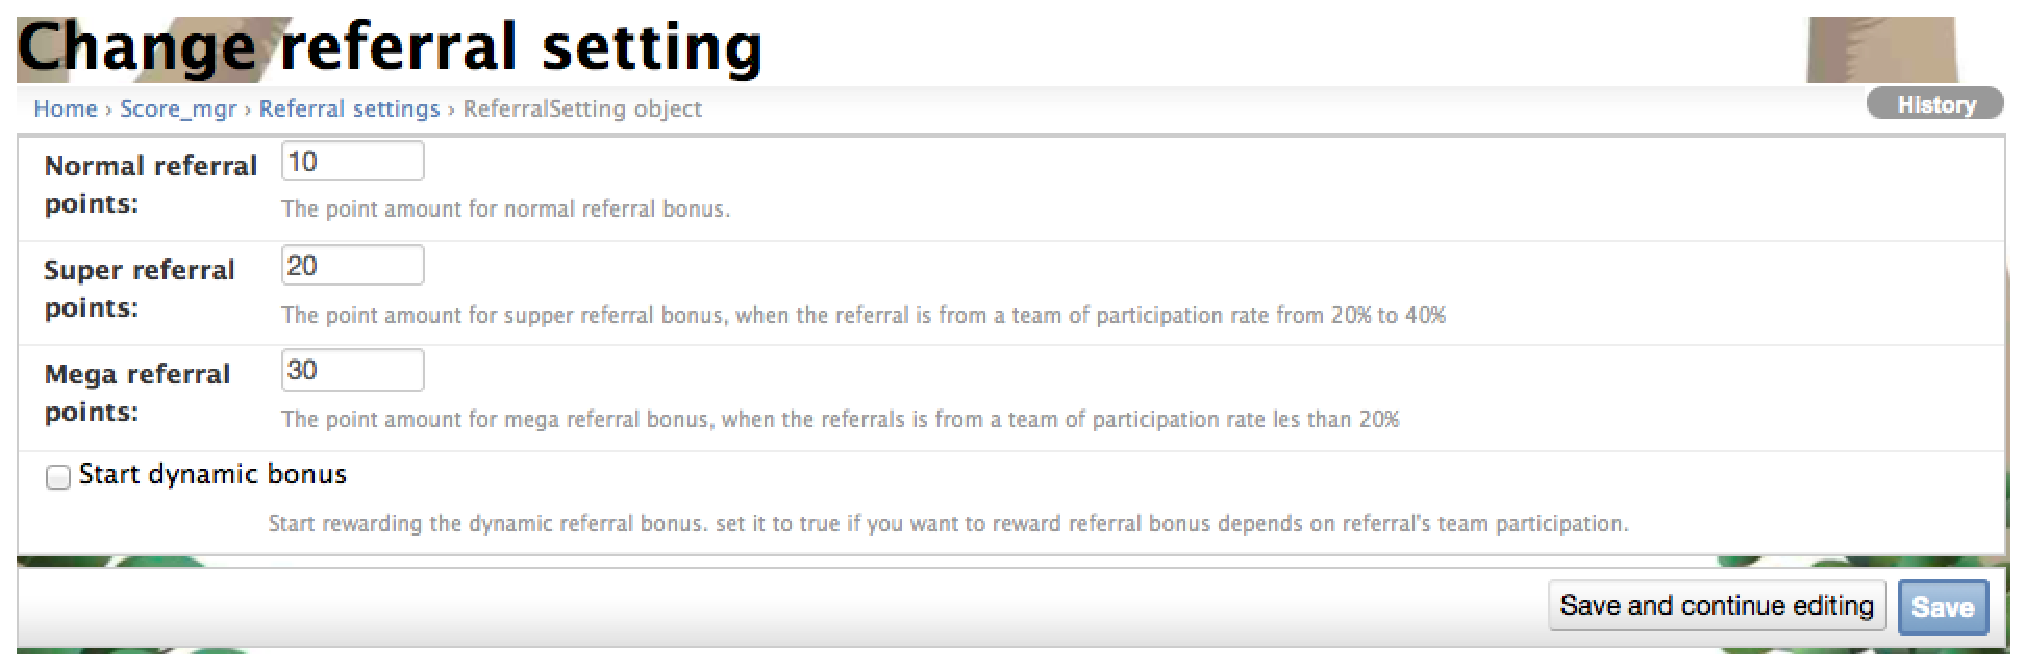
\includegraphics[width=0.85\columnwidth]{referral-change.eps}
  \caption{\em Changing the Referral Bonus Game Mechanics Settings}
  \label{fig:referral-change}
\end{figure}

By default, only the ``Normal'' referral points value is used. If you check the ``Start dynamic bonus'' setting, then the ``Super'' and ``Mega'' values are enabled depending upon the team participation rate of the new player.

\clearpage

\subsection{Configurable resource}
In Makahiki, different resources can be tracked and configured. The admin interface is built in to support the configuration of different resources. Makahiki supports three kinds of resources: energy, water, waste, which have different attributes. Some resource data can be obtained automatically from smart meters, while some resource data has to be input manually. In the case of manually data entry, the time of manual entry can be configured as well. Figure \ref{fig:resource} shows the Makahiki admin interface to configure the resources.

\begin{figure}[!ht]
	\centering
		\subfigure[Supported resource types]{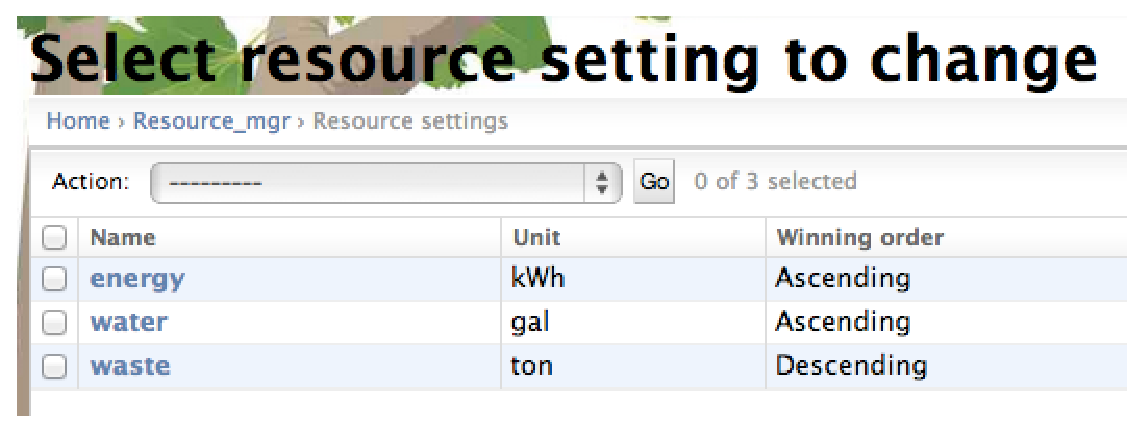
\includegraphics[width=0.7\columnwidth]{resource.eps}}
		\subfigure[Manual resource]{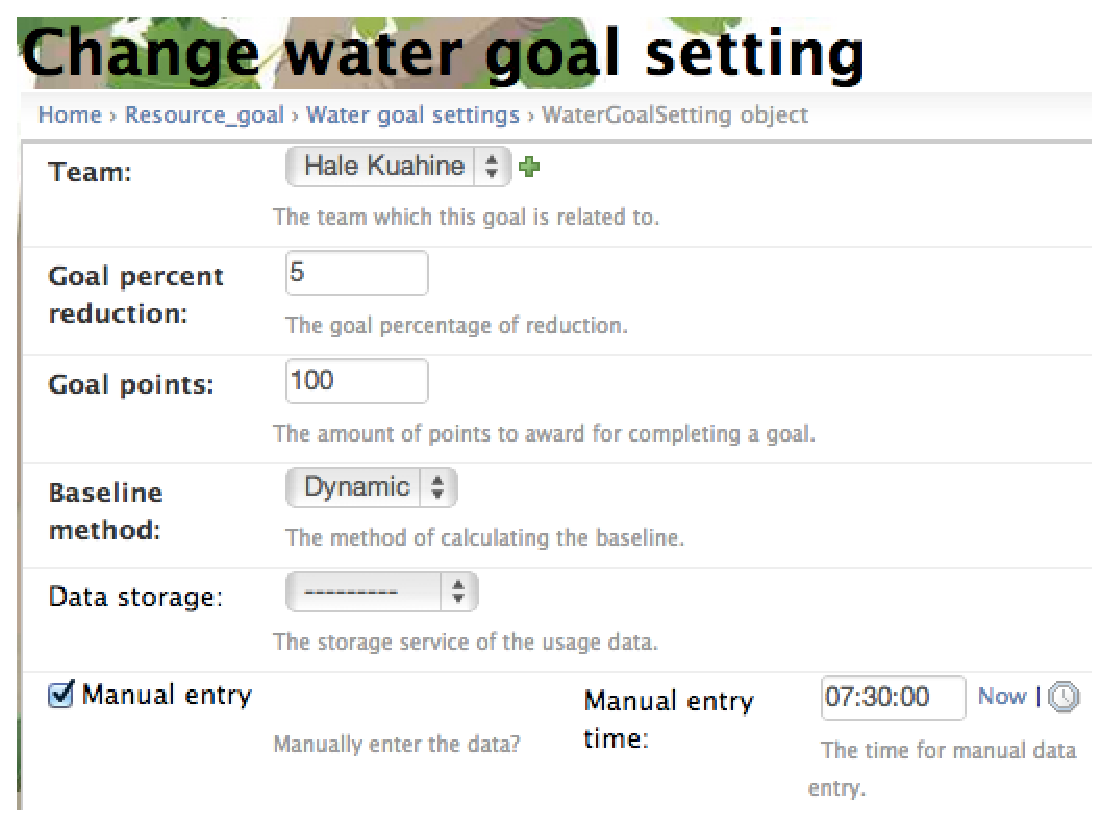
\includegraphics[width=0.7\columnwidth]{goalsettings.eps}}
		\caption{Configurable resource}
		\label{fig:resource}
\end{figure}

Makahiki supports both automated and manual data collection. With respect to automated energy collection, Makahiki queries a WattDepot server once an hour to get an update on each team's consumption during the previous hour, and then updates the stoplight visualization. At midnight, Makahiki determines whether the conservation goal was achieved by the team and updates the calendar-based view with the results for that day.

However, not all challenge player communities have meters that are internet-accessible and thus allow this kind of real-time, automated update. Instead, they might have a traditional, analog meter.

The Energy Goal Game can be configured to support manual data collection. To accomplish this, the challenge designers must first tell the system the time each day at which they will read the meters manually. (To make the energy goal game workable, the challenge designers must commit to reading the energy meters for each team at approximately the same time each day so Makahiki can assume the data represents equal, 24 hour intervals. Team meters can be read at different times, but the time must be consistent for each team.)

Then, each day during the challenge, the challenge designers read the meters, then login to the system and update Makahiki with the latest readings. From this, Makahiki can determine which teams made their energy goal for the previous day.

From a user interface perspective, the basic difference is that the stoplight visualization is not available. Instead, the primary interface to the Energy Goal Game is the calendar-based visualization, which shows the results for each day.

Once we had support for both automated and manual energy data collection,  we could also support Water Goal Games, Food Goal Games, Waste Goal Games, or any other ``resource'' for which teams are responsible. Currently, Makahiki provides built-in support for two resource goal games: energy and water. Each of those games, when enabled, results in a page devoted to that resource in the web application. The default configuration enables support for the Water Goal Game and the Water page.

Extending Makahiki to support an additional resource goal game is straightforward, but requires developer-level capabilities.

\subsection{Real-time Analytics}

Makahiki is designed to support energy challenges involving hundreds or thousands of users lasting weeks or months.  In these circumstances, effective use of the technology requires the ability to understand the state of the game, such as: Who is using it? What are they doing? What is the player response to activities, commitments, excursions, and events?   Such state information is important for planning purposes, such as assessing the transportation needs for an upcoming excursion by seeing how many players signed up.   It can also be used for making in-game changes to game design, such as changing the point values associated with activities to encourage or discourage participation.  It can also help identify breakdowns in game play, such as significant numbers of unallocated raffle tickets indicating that users do not understand the nature of that game mechanic.

To address these needs and others, Makahiki includes a variety of widgets that work together to provide high level overview of game play state to the administrators of a challenge. Figure \ref{fig:status} shows an example of two game analytic widgets.

\begin{figure}[!ht]
  \center
  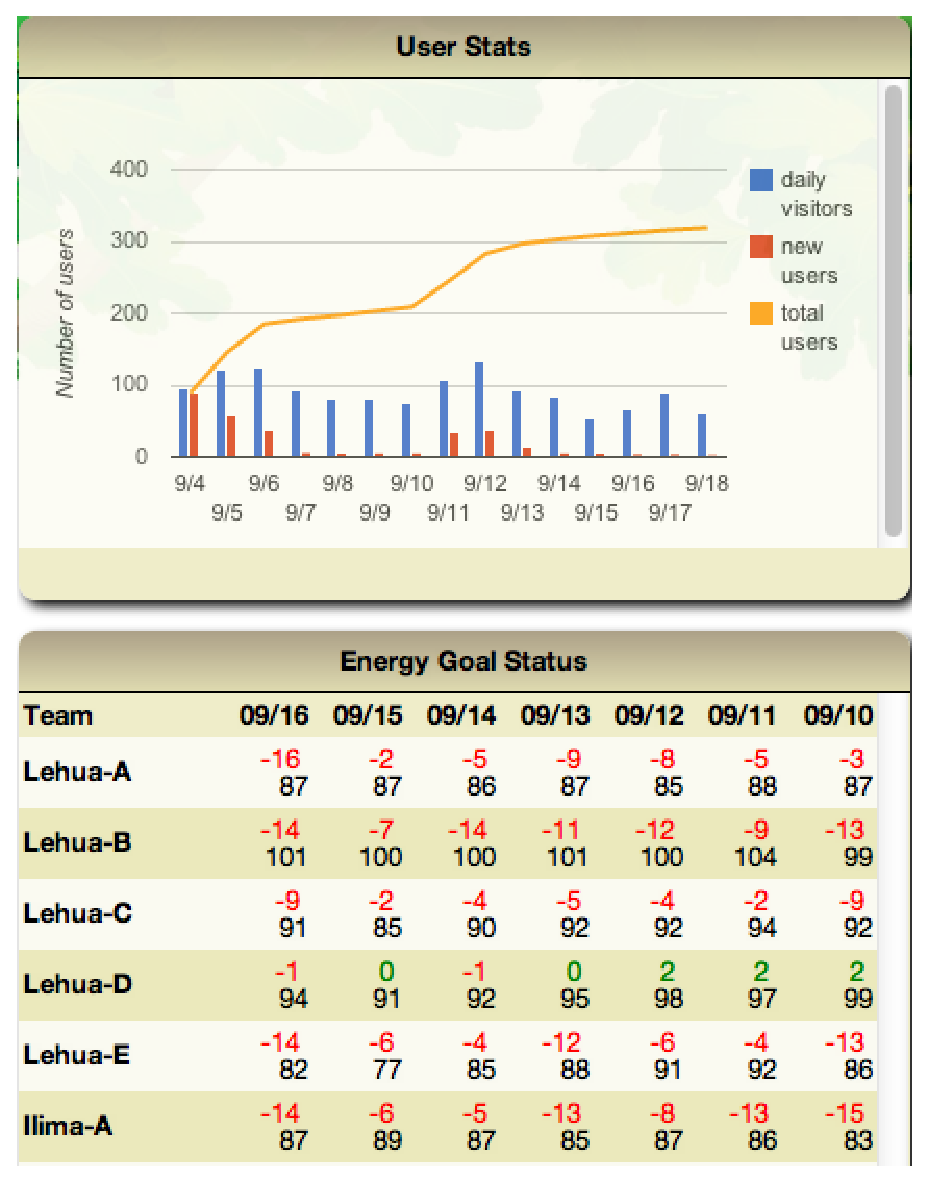
\includegraphics[width=0.7\columnwidth]{status.eps}
  \caption{Game analytic widgets: User Stats and Energy Goal Status}
  \label{fig:status}
\end{figure}

The top widget, User Stats, shows trends in the total number of players, the total number of new users, and the total number of players visiting the site each day.  The bottom widget provides information on the ability of teams to achieve their daily energy goal each day and over time.

\clearpage

\subsection{Responsive mobile support}
We believe that mobile support is essential for this kind of sustainability challenge, especially for the new generation players. Makahiki implemented the responsive web design technology to support multiple devices, to enhance the players experience. Figure\ref{fig:responsive} shows the responsive interface in Makahiki that supports both desktop view and mobile view with the same code base.

\begin{figure}[!ht]
  \center
  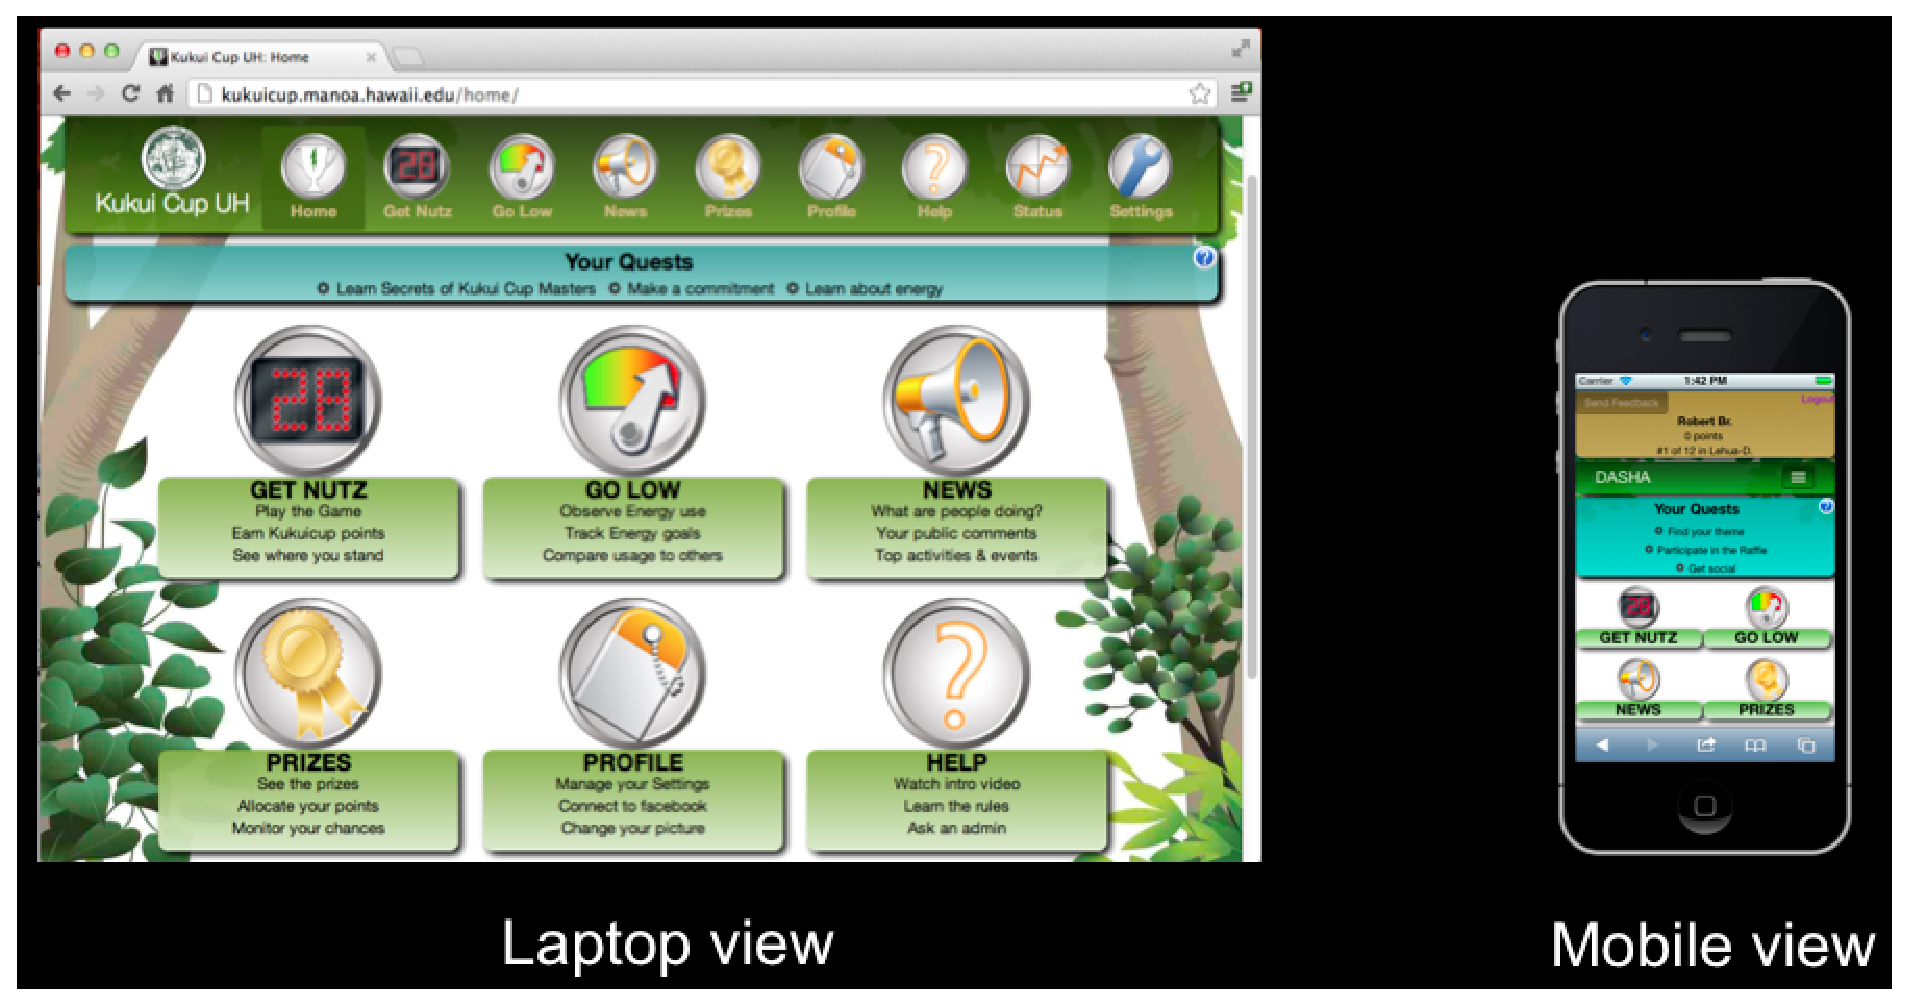
\includegraphics[width=0.9\columnwidth]{responsive.eps}
  \caption{Responsive design supports both desktop and mobile}
  \label{fig:responsive}
\end{figure}

\clearpage

\subsection{Cloud deployment support}
Another feature we implement in Makahiki is the ability to deploy to the Cloud platform. Cloud computing has the advantage of simplify IT administration by eliminating the need of acquiring the hardware, installing software etc, thus lower the cost of the software deployment. Figure\ref{fig:heroku} shows a screen shot of the Dashboard showing the 2012 East West center Kukui challenge deployed in the Heroku, one of the cloud platform provider. The monthly cost for the IT infrastructure in this instance is fairly affordable. 

\begin{figure}[!ht]
  \center
  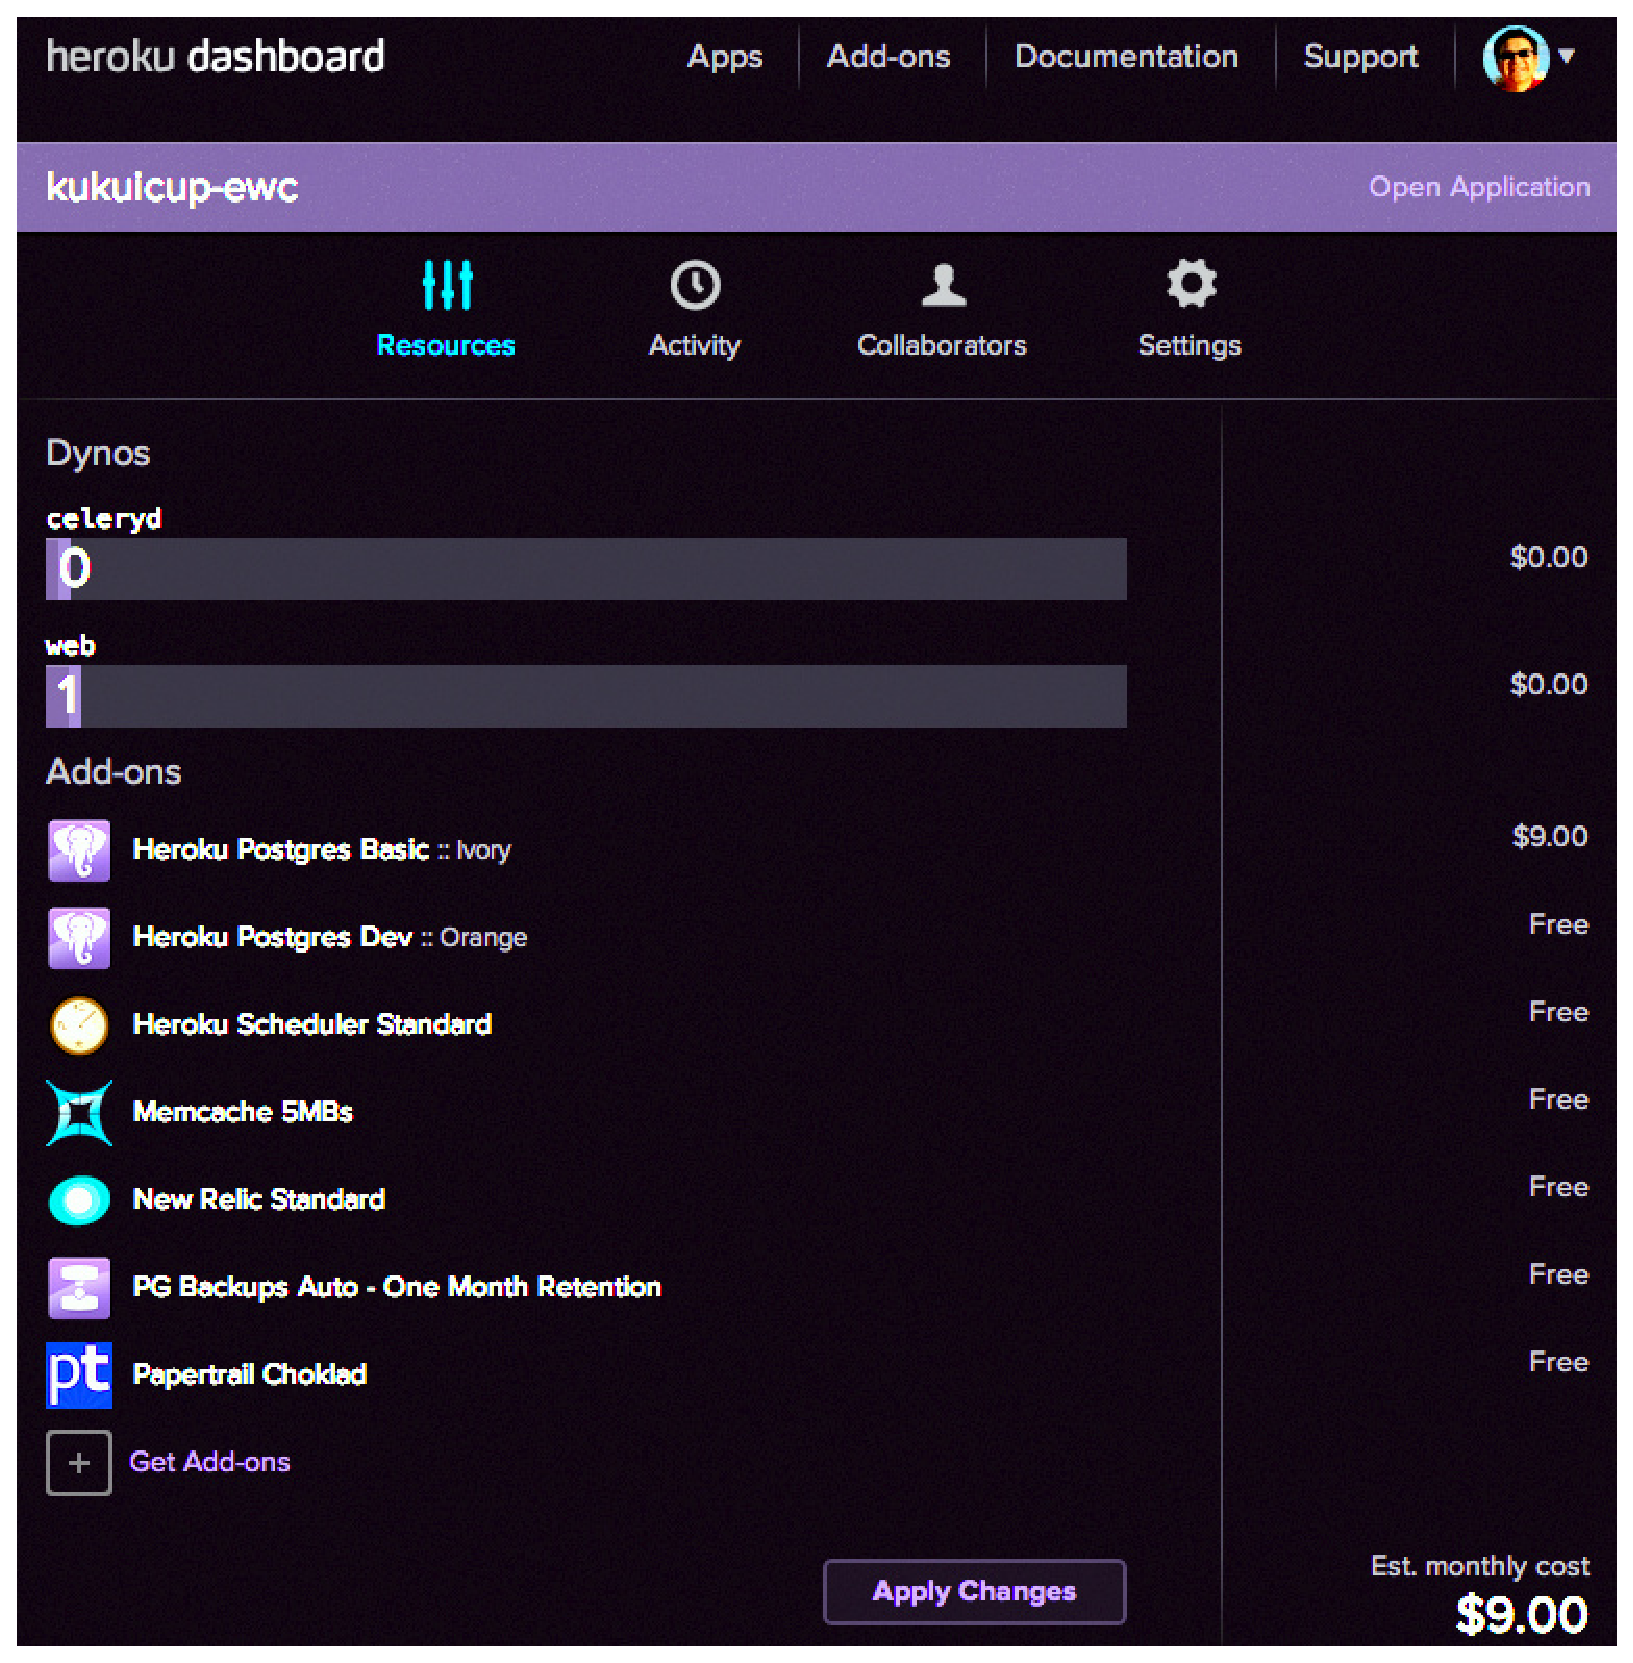
\includegraphics[width=0.8\columnwidth]{heroku.eps}
  \caption{Heroku cloud deployment}
  \label{fig:heroku}
\end{figure}

\clearpage

\subsection{Customization and Extension Development Support}
Makahiki, as a framework, provides facilities to help developers to create customization and extension to fit different requirements from  organization. The following section describes the two customization that can be implemented by developers through minimum programming.

\subsubsection{Theme Development}
A ``theme'' in Makahiki consists of a specification of the background image (or color), as well as with the background and font colors for various structural elements of the system. Players have the ability to select themes from the Profile page, making it unnecessary to develop a ``perfect'' theme for your challenge. Figure \ref{fig:theme-change} shows the widget that a player can change the theme they like the best for their personal website feel. 

\begin{figure}[!ht]
  \center
  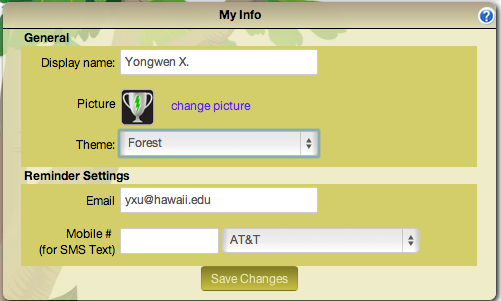
\includegraphics[width=0.6\columnwidth]{theme-change}
  \caption{Change the Website Theme}
  \label{fig:theme-change}
\end{figure}

Makahiki provides a set of pre-built themes for players to choose from. Figure \ref{fig:theme-installed} lists all the installed themes in Makahiki. These installed themes will show up in the ``Theme'' drop-down that can be selected by a player as shown in Figure \ref{fig:theme-change}.

\begin{figure}[!ht]
\begin{lstlisting}
##########################################################
# INSTALLED Themes. Please keep them in alphabetical order
##########################################################
INSTALLED_THEMES = (
    'theme-bubbles',
    'theme-bumblebee',
    'theme-forest',
    'theme-google',
    'theme-hpu',
    'theme-revolusun',
    'theme-sonora',
    'theme-space',
    'theme-wave',
)
\end{lstlisting}
\caption{Makahiki Pre-Built Themes Defined in settings.py}
\label{fig:theme-installed}
\end{figure}

Makahiki, as a framework, allows developers to create additional themes. Makahiki's themes are implemented using LESS, which is the  enhanced version of CSS that supports variables and other capabilities not available in standard CSS. There is no need to know about LESS in order to create Makahiki themes. Most developers should be able to create themes simply by copying and editing a pre-existing theme file and changing some of the LESS variables in the new file. All the theme files are located in the ``makahiki/static/less'' directory.  Most of the times, a theme developer only needs to pick the color for the theme and specify which color he want for a specific UI elements in the LESS file. Figure \ref{fig:theme-google-less} shows a snippet of the theme-google.less file.

\begin{figure}[!ht]
\begin{lstlisting}
// Google color palette
@google-white:          #FFFFFF;
@google-offwhite:       #E9EEF5;
@google-lightblue:      #8DAAEB;
@google-gold:           #E8AC13;
@google-lightlightblue: #B8CAE0;
@google-darkblue:       #1249E0;
@google-red:            #D41C34;

// Page Background
@use-bkg-image: false;
//@page-bkg-image: "../images/forest-theme-background.jpg";

@page-bkg-color-start: @google-white;
@page-bkg-color-end: @google-white;
@page-font-color: @black;
@page-link-color: @google-darkblue;

// Widgets
@widget-title-bkg-color-start: @google-lightblue;
@widget-title-bkg-color-end: @google-lightblue;
@widget-title-font-color: @black;
@widget-title-transparency: 0%;
@widget-body-bkg-color: @google-white;
@widget-body-font-color: @black;
@widget-body-transparency: 0%;

// Smart grid game
@sgg-header-bkg-color: @google-offwhite;
@sgg-header-font-color: @black;
@sgg-entry-font-color: @black;
@sgg-activity-cell-bkg-color: @google-lightblue;
@sgg-commitment-cell-bkg-color: @google-red;
@sgg-event-cell-bkg-color: @google-gold;
@sgg-excursion-cell-bkg-color: @google-darkblue;
@sgg-filler-cell-bkg-color: lighten(@black, 30%);

\end{lstlisting}
\caption{theme-google.less Defines the Google Theme}
\label{fig:theme-google-less}
\end{figure}

Once the theme file are created, it should be included in the ``INSTALLED\_THEMES'' section in the settings.py file as shown in the previous Figure \ref{fig:theme-installed}. To see the results of the new theme, Makahiki provides a special page called �theme-display�. The developer can use the browser to go to this page to test all of the theme-able elements in a single page. Figure \ref{fig:theme-google-test} illustrates the result of the new theme.

\begin{figure}[!ht]
  \center
  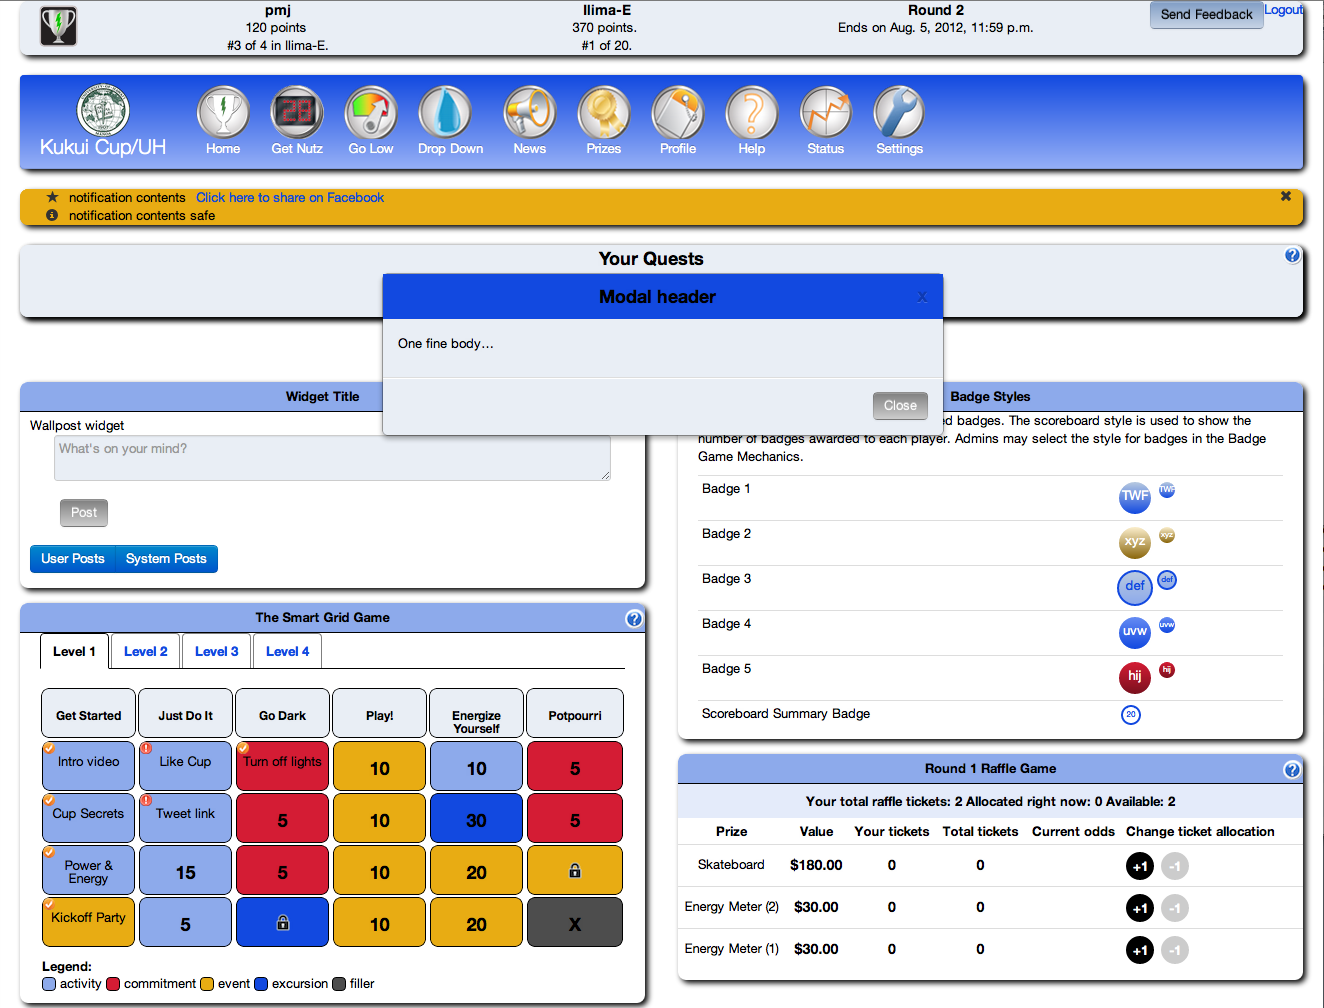
\includegraphics[width=0.99\columnwidth]{theme-google}
  \caption{The Result of theme-google.less}
  \label{fig:theme-google-test}
\end{figure}

\clearpage

\subsubsection{New Game Widget Development Support}

As discussed before, Makahiki includes a set of pre-built game and game mechanics widgets for game designers to select and configure for their serious game challenges. In some cases, game designers may wish to implement additional games or mechanics and integrate into the Makahiki system. It is achievable by the new game widget development support from the Makahiki framework. It is done in the programming level by developers. As we know that Makahiki is developed using Python and the Django web application framework, in order to develop new games, programming knowledge of Python and Django is required. This is unlike the theme development where there is no need to know LESS or any programming, 

Developing a new widget for Makahiki includes the following four steps::

The {\bf First Step} is to create the new widget package structure. Makahiki provides a command line tool called ``startwidget'' integrated into the standard Django manage.py utility. It is the easiest way to create the basic file structure for a new widget . Figure \ref{fig:startwidget} illustrates the command to create a hello\_world widget and the base files and directory structure that are created by the tool. 

\begin{figure}[!ht]
\begin{lstlisting}
% manage.py startwidget hello_world
\end{lstlisting}
\begin{lstlisting}
hello_world/
            __init__.py
            views.py
            tests.py
            templates/
                      index.html
\end{lstlisting}
\caption{Makahiki Tool for Creating a New Widget Structure}
\label{fig:startwidget}
\end{figure}

The command creates a directory named after the new widget in the directory ``apps/widgets'', and four files underneath:
\begin{itemize}
\item {\em \_\_init\_\_.py}: this file indicates that the directory is a Python package.
\item {\em views.py}: this file implements the widget logic and provide data to the UI.
\item {\em index.html}: this file defines the UI that displayed to players.
\item {\em tests.py}: this file provides the skeleton of the unit testing for the new widget.
\end{itemize}

These files are the starting points for building a new widget. The subsequent steps describe their usage in details.

The {\bf Second Step} is to implement the logic of the widget and provide the data for display. It is done in the views.py by calling the Application Programming Interfaces (APIs) provided by Makahiki. 

Makahiki API provides a generic mechanism for supply data for display.  When the player loads a page, the Makahiki module ``{\bf apps.pages.views.index}'' is called. This module determines the name of the page dynamically and creates a Python dictionary, called ``{\bf view-objects}''.  From the page configuration, it determines which widgets are enabled for the given page. It then loops over each widget and calls their ``{\bf apps.widgets.widget\_name.views.supply}'' function. So the entry point for the widget is the supply function in its views.py file. 

The startwidget command provides the empty supply function in the views.py it created, as shown in Figure \ref{fig:views}. 
\begin{figure}[!ht]
\begin{lstlisting}
"""Provides the view of the widget."""
def supply(request, page_name):
    """ supply view_objects for widget rendering."""
    _ = request
    _ = page_name
    return {}
\end{lstlisting}
\caption{supply function template provided in the views.py}
\label{fig:views}
\end{figure}

A developer needs to fill in the supply function to provide the data. Makahiki also includes a library of manager modules that provide the APIs to interact with the system. Table \ref{table:managers} lists all the manager modules and their functionality. 

For illustration purpose, the hello\_world widget will display three kind of data obtained from the Makahiki system. One is the name of the player, which is stored in the name attribute of profile object. The second is the name of the team the player belongs to. It is stored in the team attribute of the profile object. The third data is the current point score of the player. It can be retrieved from calling the function ``player\_points'' in the ``score\_mgr'' module. Figure \ref{fig:views-example} shows the complete example of views.py for hello\_world widget.

\begin{figure}[!ht]
\begin{lstlisting}
"""Provide the view for the Hello_World widget."""
from apps.managers.score_mgr import score_mgr
def supply(request, page_name):
    """Supply view_objects contents, which are the player name, team and points."""
    _ = page_name
    profile = request.user.profile
    name = profile.name
    team = profile.team
    points = score_mgr.player_points(profile)
    return {
        "name": name,
        "team": team,
        "points": points,
    }
\end{lstlisting}
\caption{An complete example of views.py}
\label{fig:views-example}
\end{figure}

The {\bf Third Step} in create a new widget is to define the UI component. It is done in the index.html under the templates directory.
Figure \ref{fig:index-base} shows the base index.html created by the startwidget command.

\begin{figure}[!ht]
\begin{lstlisting}
<div class="content-box">
    <div class="content-box-title">
        Widget name
    </div>
    <div class="content-box-contents">
        Widget content
    </div>
</div>
\end{lstlisting}
\caption{The base index.html}
\label{fig:index-base}
\end{figure}

Makahiki provides many different styles and CSS classes. Normally, widgets are contained in a content-box . The context-box is a rounded, shaded box with two parts, content-box-title, and content-box-contents. A developer can replace the ``Widget name'' in the title box and the ``Widget content'' in the content box, to display the data provided from the views.py. A complete example of the index.html file of the hello\_world widget is shown in Figure \ref{fig:index-example}. The data provided from the views.py are referenced by the convention of ``{\bf view\_objects.widget\_name.variable}''.

\begin{figure}[!ht]
\begin{lstlisting}
<div class="content-box">
    <div class="content-box-title">
        Hello World Widget
    </div>
    <div class="content-box-contents">
        Welcome <b>{{ view_objects.hello_world.name }}</b>, <br/>
          you're in team <b>{{ view_objects.hello_world.team }}</b> <br/>
          you have <b>{{ view_objects.hello_world.points}}</b> points.
    </div>
</div>
\end{lstlisting}
\caption{An complete example of index.html}
\label{fig:index-example}
\end{figure}

Finally, the {\bf Fourth Step} for developing a new widget is to add the widget to a page. In order for a new widget to be available to the system, you need to edit the Makahiki ``settings.py'' file and add the widget name to the INSTALLED\_WIDGET\_APPS variable. Figure \ref{fig:installed-widget} shows a portion of the settings.py file after adding the new hello\_world widget. 
\begin{figure}[!ht]
\begin{lstlisting}
################################
# INSTALLED Widgets
################################
INSTALLED_WIDGET_APPS = (
  'action_feedback',
  'ask_admin',
  'badge_scoreboard',
  'badges',
  'bonus_points',
  'hello_world',
  'home',
  ....
  )
\end{lstlisting}
\caption{Add the new widget to settings.py}
\label{fig:installed-widget}
\end{figure}

This last step makes the newly developed widget available to the Makahiki system. It concludes all the steps a developer needed to create a new game widget. Once it is available to the system, a game designer will be able to add the widget to an existing page using the admin interface.

The ``Page Settings'' link in the admin interface is used to configure the widgets in a page. Figure \ref{fig:page-settings} shows the hello\_world widget being added to the existing Profile page.

\begin{figure}[!ht]
  \center
  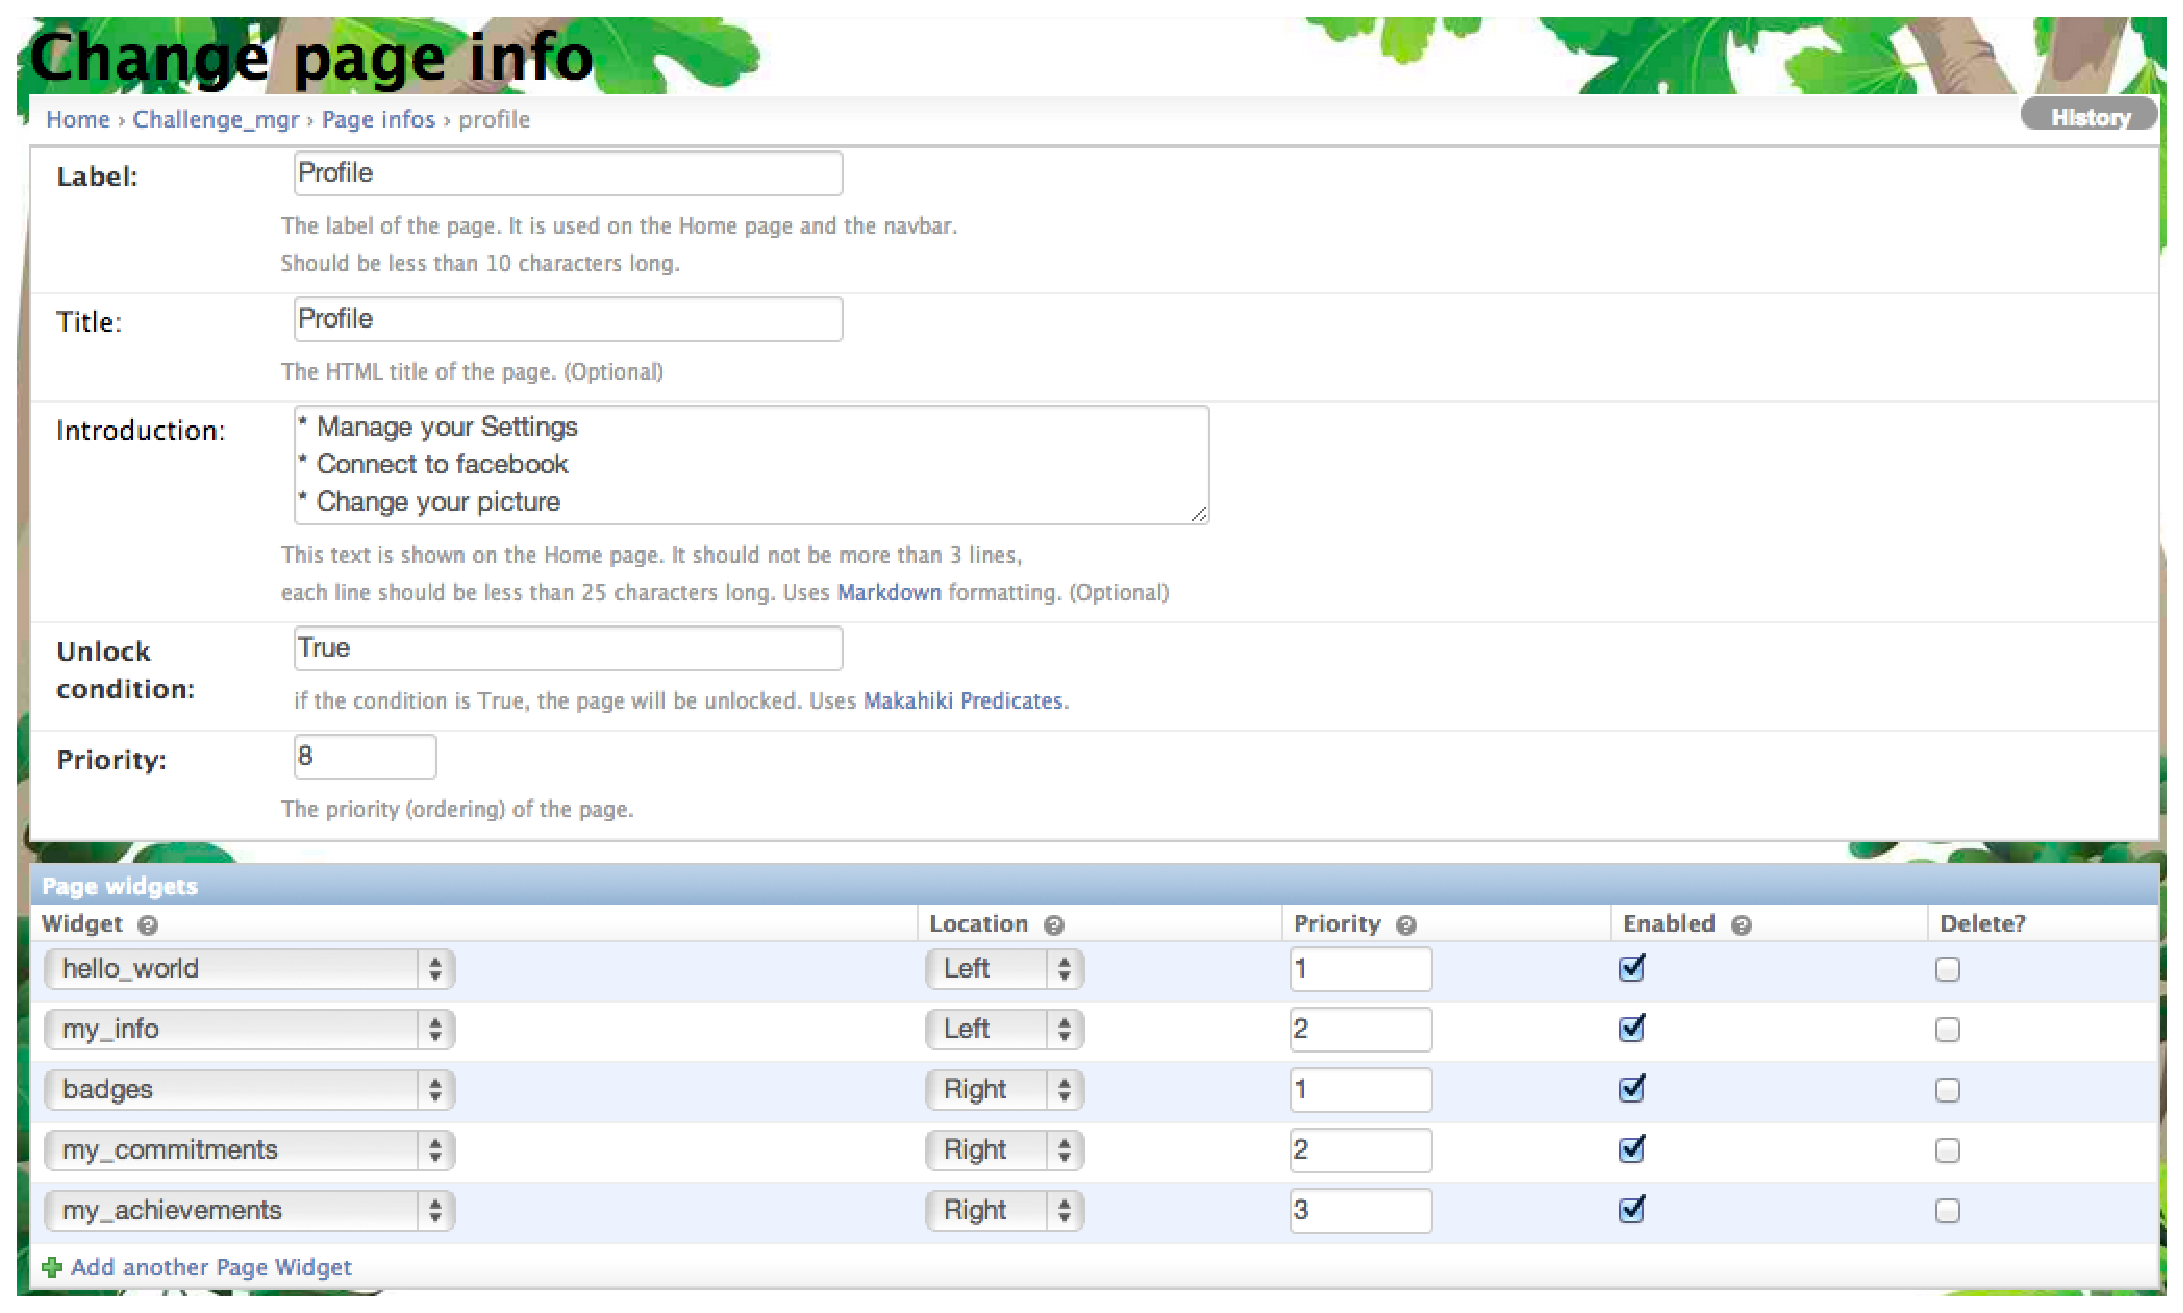
\includegraphics[width=0.99\columnwidth]{page-settings}
  \caption{The Hello World Widget added to the Left column}
  \label{fig:page-settings}
\end{figure}

The hello\_world widget is added to the left side location with the priority set to ``1'', which indicates that the new widget will be displayed first and before the ``My Info'' widget (priority 2) on the left side column on the page.  The widget will also need to be enabled by checking the ``enabled'' checkbox. Figure \ref{fig:hello-world-widget} shows the final result of the hello\_widget displayed in the Profile page.
\begin{figure}[!ht]
  \center
  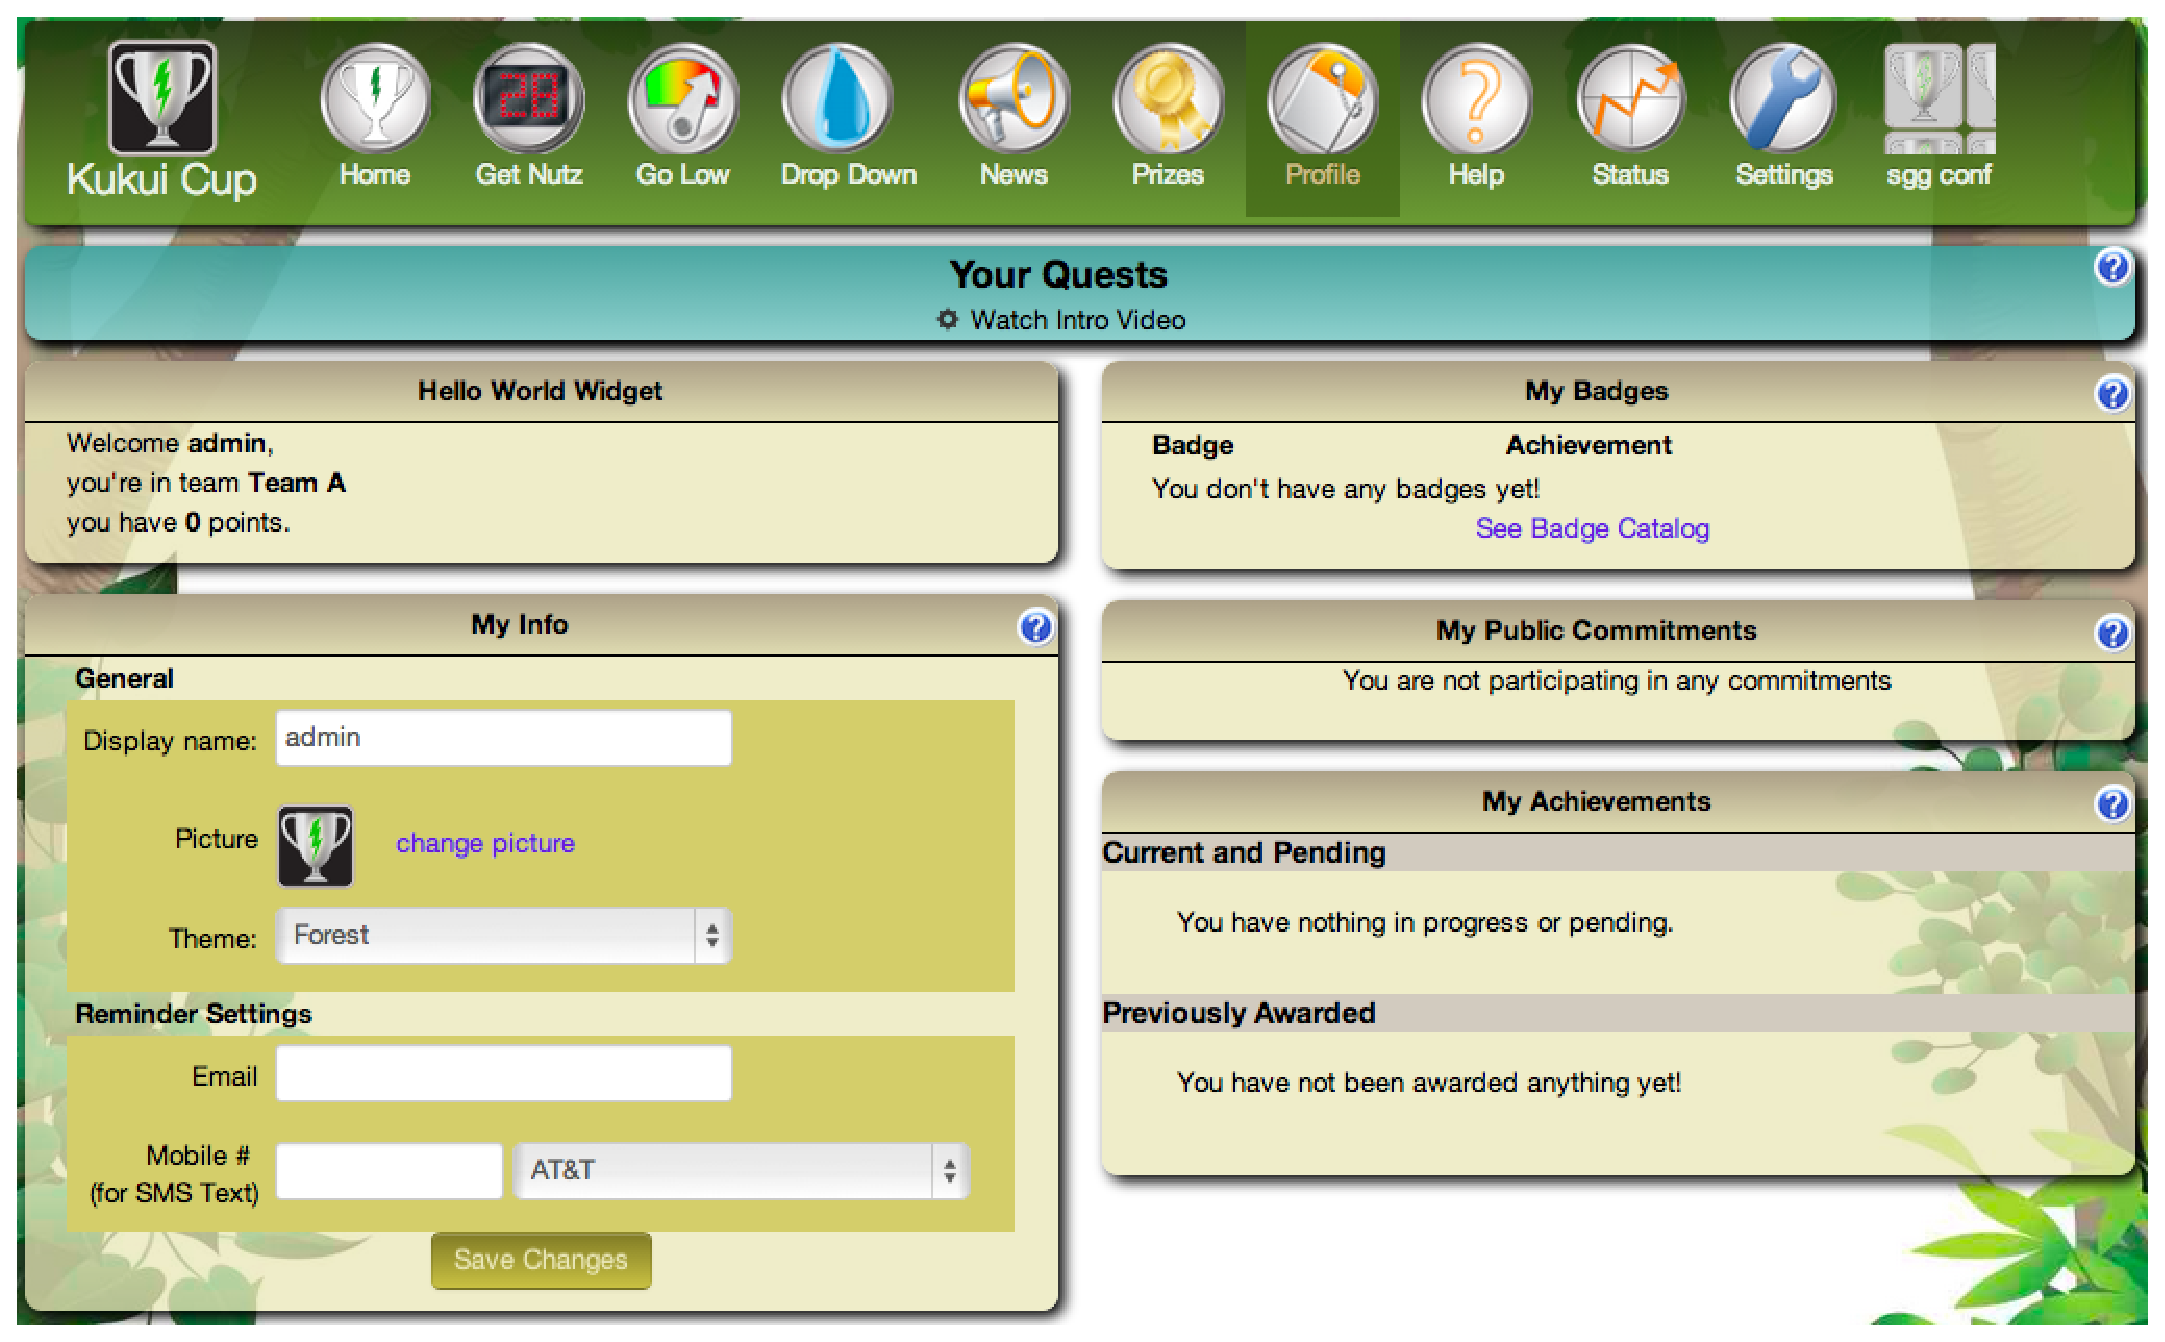
\includegraphics[width=0.99\columnwidth]{hello-world-widget}
  \caption{The Hello World Widget Displayed in the Profile page}
  \label{fig:hello-world-widget}
\end{figure}

